%% ----------------------------------------------------------------
%% Thesis.tex -- MAIN FILE (the one that you compile with LaTeX)
%% ---------------------------------------------------------------- 

% Set up the document
\documentclass[a4paper, 11pt, oneside]{Thesis}  % Use the "Thesis" style, based on the ECS Thesis style by Steve Gunn

\usepackage[titletoc]{appendix}
\usepackage{float}
\usepackage{listings}
\usepackage{verbatim}
\usepackage{courier}
% Include any extra LaTeX packages required
\usepackage[square, numbers, comma, sort&compress]{natbib}  % Use the "Natbib" style for the references in the Bibliography

\usepackage[utf8]{inputenc}
\usepackage[greek,english]{babel}
\usepackage{lmodern}	

\usepackage{mathtools, nccmath}
\usepackage[nottoc]{tocbibind} % bind bibliography to the table of contents
\usepackage{verbatim}  % Needed for the "comment" environment to make LaTeX comments
\usepackage{vector}  % Allows "\bvec{}" and "\buvec{}" for "blackboard" style bold vectors in maths
\usepackage[table]{xcolor}


\hypersetup{urlcolor=black, colorlinks=true}  % Colours hyperlinks in black, can be distracting if there are many links and colored blue.

\makeatletter
\let\c@table\c@figure % for (1)
\let\ftype@table\ftype@figure % for (2)
\makeatother

%% ----------------------------------------------------------------

\begin{document}
\frontmatter      % Begin Roman style (i, ii, iii, iv...) page numbering

% Set up the Title Page
\title  {Real-Time Monitoring of Message-Driven Data Pipelines}
\authors  {John McAleer}
            
\addresses  {\groupname\\\deptname\\\univname}  % Do not change this here, instead these must be set in the "Thesis.cls" file, please look through it instead
\date       {\today}
\subject    {}
\keywords   {}


\maketitle
%% ----------------------------------------------------------------

\setstretch{1.3}  % It is better to have smaller font and larger line spacing than the other way round

% Define the page headers using the FancyHdr package and set up for one-sided printing
\fancyhead{}  % Clears all page headers and footers
\rhead{\thepage}  % Sets the right side header to show the page number
\lhead{}  % Clears the left side page header

\pagestyle{fancy}  % Finally, use the "fancy" page style to implement the FancyHdr headers
%% ----------------------------------------------------------------
% Declaration Page required for the Thesis, your institution may give you a different text to place here


\Declaration{

\addtocontents{toc}{\vspace{1em}}  % Add a gap in the Contents, for aesthetics

I, John McAleer, declare that this proposal titled, `Real-Time Monitoring of Message-Driven Data Pipelines' and the work presented in it are my own. I confirm that:

\begin{itemize} 
\item[\tiny{$\blacksquare$}] This work was done wholly or mainly while in candidature for an masters degree at Cork Institute of Technology.
 
\item[\tiny{$\blacksquare$}] Where I have consulted the published work of others, this is always clearly attributed.
 
\item[\tiny{$\blacksquare$}] Where I have quoted from the work of others, the source is always given. With the exception of such quotations, this project report is entirely my own work.
 
\item[\tiny{$\blacksquare$}] I have acknowledged all main sources of help.
 
\item[\tiny{$\blacksquare$}] I understand that my project documentation may be stored in the library at CIT, and may be referenced by others in the future.
\\
\end{itemize}
 
 
Signed:\\
\rule[1em]{25em}{0.5pt}  % This prints a line for the signature
 
Date:\\
\rule[1em]{25em}{0.5pt}  % This prints a line to write the date
}
\clearpage  % Declaration ended, now start a new page

%% ----------------------------------------------------------------

% The Abstract Page

\addtotoc{Abstract}  % Add the "Abstract" page entry to the Contents

\abstract{
\addtocontents{toc}{\vspace{1em}}  % Add a gap in the Contents, for aesthetics

The Message-Driven Architecture (MDA), a subset of the Service-Oriented Architecture (SOA), is an architectural pattern applied to the design of applications comprising loosely-coupled software components which communicate over a messaging system. Message-driven applications  comprise sets of message producers, message consumers and message sinks, communicating over a set of message channels. The decoupling inherent to message-driven applications provides a high degree of structural malleability; message producers are unaware of message consumers, enabling the addition and removal of software components with minimal impact. This architecture is commonly employed in the implementation of data pipelines, systems which comprise multiple services responsible for the ingestion, validation, transformation and processing of continuous streams of data.

Given the decoupled and flexible nature of the Message Driven Architecture, identification of the set of services comprising a pipeline, the communication paths between same, and the characteristics of runtime service intercommunication at a point in time may present a number of difficulties. Developers, testers, and maintainers of message-driven pipeline applications face such challenges during all stages of the development and production life-cycle. 

This thesis explores contemporary practices and technologies in the area of message-driven pipeline monitoring. The technical challenges inherent to the design and implementation of a real-time monitoring solution are explored. A technology-agnostic monitoring application is developed and successfully applied to an Apache Kafka-based messaging pipeline. 



\clearpage  % Abstract ended, start a new page
%% ----------------------------------------------------------------

\setstretch{1.3}  % Reset the line-spacing to 1.3 for body text (if it has changed)

% The Acknowledgements page, for thanking everyone
\acknowledgements{
\addtocontents{toc}{\vspace{1em}}  % Add a gap in the Contents, for aesthetics

The author wishes to express wholehearted appreciation to Dr. Donna Griffin of the CIT Computer Science Department for her assistance and guidance in the development of this dissertation from concept to submission, and to Mr. Larkin Cunningham for his valuable feedback.
}
\clearpage  % End of the Acknowledgements
%% ----------------------------------------------------------------

\pagestyle{fancy}  %The page style headers have been "empty" all this time, now use the "fancy" headers as defined before to bring them back


%% ----------------------------------------------------------------
\lhead{\emph{Contents}}  % Set the left side page header to "Contents"
\tableofcontents  % Write out the Table of Contents

%% ----------------------------------------------------------------
\lhead{\emph{List of Figures}}  % Set the left side page header to "List if Figures"
\listoffigures  % Write out the List of Figures

%% ----------------------------------------------------------------
\lhead{\emph{List of Tables}}  % Set the left side page header to "List of Tables"
\listoftables  % Write out the List of Tables

%% ----------------------------------------------------------------

%% ----------------------------------------------------------------
\setstretch{1.5}  % Set the line spacing to 1.5, this makes the following tables easier to read
\clearpage  % Start a new page
\lhead{\emph{Abbreviations}}  % Set the left side page header to "Abbreviations"
\listofsymbols{ll}  % Include a list of Abbreviations (a table of two columns)
{
	% \textbf{Acronym} & \textbf{W}hat (it) \textbf{S}tands \textbf{F}or \\
	\textbf{API} & \textbf{A}pplication \textbf{P}rogramming \textbf{I}nterface \\
	\textbf{CEP} & \textbf{C}omplex \textbf{E}vent \textbf{P}rocessing  \\
	\textbf{CRUD} & \textbf{C}reate, \textbf{R}etrieve, \textbf{U}pdate, \textbf{D}elete \\
	\textbf{CPU} & \textbf{C}entral \textbf{P}rocessing \textbf{U}nit \\
	\textbf{DAO} & \textbf{D}ata \textbf{A}ccess \textbf{O}bject \\
	\textbf{DTO} & \textbf{D}ata \textbf{T}ransfer \textbf{O}bject \\
	\textbf{HTTP} & \textbf{H}yper\textbf{T}ext \textbf{T}ransfer \textbf{P}rotocol \\
	\textbf{IoT} & \textbf{I}nternet \textbf{o}f \textbf{T}hings \\
	\textbf{ITOM} & \textbf{IT} \textbf{O}perations \textbf{M}anagement \\
	\textbf{JMX} & \textbf{J}ava \textbf{M}anagement \textbf{E}xtensions \\
	\textbf{JPA} & \textbf{J}ava \textbf{P}ersistence \textbf{A}PI \\
	\textbf{JSON} & \textbf{J}ava\textbf{S}cript \textbf{O}bject \textbf{N}otation \\
	\textbf{MDA} & \textbf{M}essage-\textbf{D}riven \textbf{A}rchitecture \\
	\textbf{ML} & \textbf{M}achine \textbf{L}earning \\
	\textbf{MSA} & \textbf{M}icro\textbf{S}ervice \textbf{A}rchitecture \\
	\textbf{OCL} & \textbf{O}bject \textbf{C}onstraint \textbf{L}anguage \\
	\textbf{REST} & \textbf{RE}presentational \textbf{S}tate \textbf{T}ransfer \\
    \textbf{SARESA} & \textbf{S}sense \textbf{A}nd \textbf{RE}sponse  \textbf{S}ervice \textbf{A}rchitecture\\
	\textbf{SOA} & \textbf{S}service-\textbf{O}riented \textbf{A}rchitecture \\	
	\textbf{UI} & \textbf{U}ser \textbf{I}nterface \\
	\textbf{URL} & \textbf{U}niform \textbf{R}esource \textbf{L}ocator \\
	\textbf{UUID} & \textbf{U}niverally  \textbf{U}nique \textbf{I}dentifier \\	
}

%% ----------------------------------------------------------------
\clearpage  % Start a new page


%% ----------------------------------------------------------------
% End of the pre-able, contents and lists of things
% Begin the Dedication page

\setstretch{1.3}  % Return the line spacing back to 1.3

\pagestyle{empty}  % Page style needs to be empty for this page
\dedicatory{Dedicated to Niamh, Frieda and Roisin; to their boundless patience and light spirits.}

\addtocontents{toc}{\vspace{2em}}  % Add a gap in the Contents, for aesthetics

%%


\mainmatter	  % Begin normal, numeric (1,2,3...) page numbering
\pagestyle{fancy}  % Return the page headers back to the "fancy" style

\chapter{Introduction}
\lhead{\emph{Introduction}}

\section{Motivation}\label{intro_motivation}
The author's professional industrial experience as a designer and developer of message-driven data pipeline software has lead to some frustration at the scarcity of pipeline monitoring tooling, specifically in the areas of real-time pipeline topology discovery and message activity reporting. Major cloud providers currently provide no such monitoring functionality off the shelf, while those third party solutions that do exist often require  lock-in to a full life-cycle ecosystem, invasive instrumentation, or integration of pipeline software with complex frameworks. The author has undertaken this research in order to explore the potential for a lightweight, non-invasive and technology-agnostic solution that allows parties involved with the development of data pipelines to achieve the following fundamental use case:

\textit {As a developer, I want to understand the composition and activity state of my deployed pipeline applications at a glance}.

Wall-mounted displays used to render for example automated test results across product versions and test development environments are not uncommon in contemporary development labs. It is the author's intent that such informational dashboards will be used to convey real-time pipeline information in a format that enables developers and testers to reach conclusion about application state at a glance. Developers may ask questions such as:

\begin{enumerate}
	\item What microservices comprise the currently deployed pipelines?
	\item Which microservices are currently consumers of given a message channel or topic?
	\item Is there any message activity currently occurring in any part of a given pipeline?
	\item Where are the performance bottlenecks in the currently deployed pipelines?
\end{enumerate}

The first question listed here may give cause for surprise. However as asserted in \cite{woods2016}, given a message-driven MSA-based application comprises a number of collaborating network-accessible processes, the structure of a given pipeline might not be well understood before runtime. 

While answers to the above queries are achievable, the process of arriving at same may be time-consuming while also requiring specific skill sets. The following examples demonstrate possible means of arriving at respective conclusions to the given questions:

\begin{enumerate}
	\item If the pipeline is deployed to a cluster manager such a Kubernetes, use client command-line tooling to enumerate the currently deployed set of microservices.
	\item Inspection of software documentation (if up-to-date) may yield an answer, though product source code is a more reliable source of truth.
	\item Manually configure listener processes for every message channel defined by the pipeline; check all processes for evidence of message production.
	\item Manually sample message activity on all message channels, then calculate and compare throughput on all channels.
\end{enumerate}

This dissertation will explore the development of a monitoring solution which enables technical staff to answer the above questions - at once - in seconds, rather than minutes or hours.	

\subsection{Research Objectives} \label{intro_objectives}

The following objectives have been identified as part of this research:

\begin{enumerate}
	\item Development of a messaging-technology agnostic, plug-in based software solution for the real-time monitoring of message-driven pipeline application state.
	\item Development of Apache Kafka specific plug-ins for the aforementioned monitoring solution.
	\item Development of an Apache Kafka-based test bed pipeline and supporting tooling. 
	\item Successful demonstration of real-time monitoring against the test bed pipeline.
	
\end{enumerate}

\section{Executive Summary} \label{exec_summary}

In order to achieve the objectives stated in section \ref{intro_objectives}, a pipeline monitoring solution and accompanying test bed pipeline will be developed.

The central effort of this research will be the design and implementation of a messaging-technology agnostic  monitoring solution. The monitoring solution will enable:

\begin{itemize}
	\item Real-time discovery and rendering of pipeline structure, i.e. the services comprising a pipeline and relationships between same.
	\item Real-time rendering of message activity in monitored pipelines.
	\item Parallel monitoring and rendition of multiple pipelines. 
	\item User-friendly configuration of monitored pipeline details.
	
\end{itemize}

In keeping with the technology-agnostic natures of the solution, the monitoring prototype will be \textit{agent} and \textit{plug-in} based\cite{Maamar:2000:OSA:351936.351955}. Where possible, the solution will be non-invasive, requiring no custom configuration of those hosts or virtual machines running monitored services.

The test bed pipeline will comprise a Kubernetes cluster (a popular open-source container orchestration system), running Apache Kafka (a distributed stream processing platform) and Zookeeper (a centralised key/value store required by Zookeeper),  running a sample data pipeline comprising three Spring Boot microservices.

Finally, the test bed will be leveraged in order to demonstrate the feasibility of performing real-time monitoring on an Apache Kafka-based pipeline.

\section{Contribution}
The key contribution of this research will be potential savings in time - and implicitly cost - to organisations involved with development of message-driven data pipelines. As detailed in section \ref{intro_motivation}, the answers to simple queries around pipeline composition and activity state currently require not only time investment, but considerable expertise in various technologies. As a further contribution, this work will render hitherto obscure application composition and state information available to non-technical parties.

\section{Structure of This Document}
The opening chapter of this thesis contains introductory motivational statements, an executive summary of planned research and a brief enumeration of the contributions this undertaking endeavours to achieve. Chapter 2 will explore the characteristics and challenges inherent to message-driven application development, examine current industry practices around runtime monitoring of such software, and review recent academic literature relating to same. Chapter 3 will detail the requirements and design for a functional pipeline monitoring solution, with attention to the challenges and potential solutions that are inherent. A deep-dive into the specifics of the implemented solution is the focus of Chapter 4. A brief walkthrough of the solution is covered in Chapter 5, while the final chapter states research conclusions and lists of number of suggestions for future work. The appendices contain step-by-step guides for downloading, building and running both the monitoring software and a supporting test bed. 

All software artefacts - including the sources used to compile this document - are available at https://github.com/schmigware/monitoring-app.

 % Introduction

\chapter{Background}
\lhead{\emph{Background}}

Given the increasing prevalence of information systems and information science in general, data volumes continue to grow exponentially\cite{Devakunchari}. Much of the data consumed by information processing systems is now generated by automated processes such as networks of sensors, financial transaction management systems and telephony networks. These system produce \textit{data streams}, unbounded datasets which update continuously over time. A data stream is defined by \citeauthor{data_stream_processing} as \textit{"an ordered sequence of instances that can be read only once or a small number of times using limited computing and storage capabilities"}\cite{data_stream_processing}.

\textit{Stream processing} has emerged in recent years as an approach to the design of software systems responsible for the real-time processing of such data streams\cite{Andrade:2014:FSP:2823980}. In contrast to batch-oriented Data Warehousing systems, which typically persist volumes of data for processing at some point in the future, stream processing systems continuously consume inputs, producing corresponding and continuous streams of outputs. 

Several domains are intrinsically suited to the real-time processing of data streams; in particular, those domains in which timely response to insights yielded by real-time processing presents business value. The \textit{sense-and-respond pattern}, a concept borrowed from control theory, has been used to describe the process of deriving continuous streams of business intelligence by means of real-time stream processing\cite{Nguyen:2005:SRS:1097002.1097015}. Domains which frequently leverage the sense-and-respond pattern include financial fraud detection, threat detection, and Internet of Things (IOT) data analytics.

For financial fraud detection, minimisation of the time delta between transaction data consumption and the production of corresponding analytics or alerts is critical. \citeauthor{Nguyen:2005:SRS:1097002.1097015} have proposed an approach to financial fraud detected entitled Sense and Response Service Architecture (SARESA), underpinned by an event-driven architecture which continuously consumes data streams from a business environment\cite{Nguyen:2005:SRS:1097002.1097015}. The authors contrast their proposed design with the typical Data Warehouse architecture, which stages data streams to a persistent database in order to perform aggregation and reporting at a later time; SARESA in comparison continuously ingests, transforms, and processes events in real-time. At the implementation level, SARESA comprises a pool of independent services communicating over a shared message bus. The use of a message bus provides for decoupling of services and lends a high degree of adaptiveness to the system;  \citeauthor{Nguyen:2005:SRS:1097002.1097015} assert that "\textit{..the processing steps of a Sense and Respond loop can be flexibly changed and updated}".

An event-driven, real-time stream processing pipeline will typically comprise a set of distributed microservices, a common architectural choice in the design and implementation of data pipelines\cite{pipeline_microservices}. \citeauthor{Cerny_microservices} consider microservices in the context of the Unix design philosophy, identifying the following three qualities of the architecture\cite{Cerny_microservices}:

\begin{enumerate}
	\item A microservice performs a dedicated task, and performs it well.
	\item A microservice interoperates with other microservices.
	\item A microservice communicates with other microservices over a universal interface.
\end{enumerate}

Two factors suggesting the suitability of microservices for pipeline implementation are potential for horizontal scalability and the inherently decoupled nature of the microservices themselves\cite{Hasselbring}.  Scalability is necessary in order to minimise pipeline processing delays when dealing with high volume data streams; furthermore the ability to scale down a pipeline is desirable during periods of minimal stream volume, in order to minimise resource consumption.

Service decoupling is achieved through use of a distributed messaging system,  as proposed by  \citeauthor{Nguyen:2005:SRS:1097002.1097015}. While pipeline microservices interact with each other, they do not do so directly and are generally unaware of each other. Rather, interaction is performed using a messaging system. As such, message data defines the contract between pipeline microservices. Distributed messaging systems typically leverage a publish-subscribe model, where message producers write to a \textit{topic}, while message consumers \textit{subscribe} to a topic. Producers are unaware of the set of message consumers, and conversely, the consumer of a message or event is unaware of the producer of same. This service decoupling lends a great deal of flexibility to pipeline design, with considerable scope for pipeline evolution over time, as will be explored later in this chapter. Popular contemporary messaging systems include Apache Kafka\cite{ApacheKafka}, ActiveMQ\cite{ActiveMQ} and RabbitMQ\cite{RabbitMQ}. 

Threat detection systems perform a broadly similar function to fraud detection systems, processing data streams continuously in order to generate real-time threat alarms and response action triggers. 
Figure \ref{threat_detection_pipeline} describes a simplified threat detection pipeline.

\vspace{5mm}

\begin{figure}[H]
	\centering  
	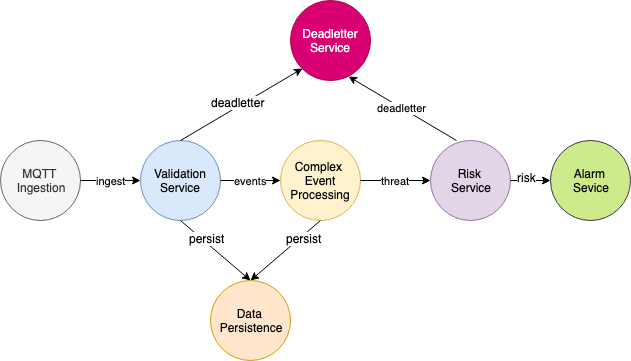
\includegraphics[scale=0.6]{figures/background/threat_detection_pipeline.png}
	\caption{Simple threat detection pipeline.}
	\label{threat_detection_pipeline}
\end{figure}

\begin{itemize}
	\item MQTT events from IoT devices are ingested at the \texttt{MQTT Ingestion Service}, transformed to an internal event/message representation, and forwarded to an \texttt{ingest} event channel.
	\item The \texttt{Validation Service} performs validation operations on events received. Some events may contain declarations of newly discovered IoT device metadata; such events will be forwarded to a \texttt{persist} event channel. Some events may represent for instance alarms generated by external IoT device such a window breakage alarm; these events are forwarded to the  \texttt{events} message channel. Uninteresting messages are discarded by forwarding them to a \texttt{Deadletter} channel.
	\item The \texttt{Complex Event Processing Service} consumes messages from \texttt{events} channel and performs processing based on for instance a rule engine definition or set of Machine Learning (ML) algorithms. Those events determined to to represent a threat are transformed to \texttt{Threat} events and forwarded to the \texttt{threat} channel. 
	\item The \texttt{Risk Service} processes incoming \texttt{Threat} events and depending on various criteria, may forward a new event on the \texttt{risk} channel.
	\item The \texttt{risk} event channel has a single consumer, the \texttt{Alarm Service}, responsible for real-time reporting of events to organisational security personnel in the event that a risk notification meeting certain criteria (for example, a numeric risk score in excess of a defined threshold) is encountered.
	
\end{itemize} 


A key aspect of this architecture is that no explicit contract is defined between microservices. As events flow through the pipeline, no event publisher is aware of consuming services. This trivialises the process of adding additional flows to a pipeline, for example:

\begin{itemize}
	\item New event types may be handled by adding an additional microservice which listeners to the \texttt{ingest} message channel.
	\item \texttt{Risk} event duplication may be eliminated by introduction of a \texttt{Correlation} microservice, which listens to the \texttt{threat} message channel, removing duplicates before fowarding to a new \texttt{threat-dedup} channel.
\end{itemize}

In order to implement these changes, the only code or configuration changes necessary for \textit{existing} microservices may be as minimal as reconfiguring the \texttt{Risk Service} to subscribe to \texttt{threat-dedup} rather than \texttt{threat} events. While this flexibility confers several benefits in terms of architectural flexibility and potential for pipeline evolution, it creates challenges with regards to determination of pipeline topology at a given moment in time, in particular during the development phase of product life-cycle.


\section{Literature Review}

While the author has reviewed several publications pertaining to discovery of Microservice Architecture based application structures, there appears to be a paucity of literature surrounding real-time topography discovery and message activity summarisation for message-driven data pipelines. What literature is extant largely explores the discovery and monitoring of microservice-based applications, a more general area.

 \citeauthor{8359145} have explored a method for automatic derivation of MSA-based application structures in \cite{8359145}. The approach described involves a combination of static service and API analysis coupled with data collection during application runtime. The system described in \cite{8359145} resembles the architecture proposed in this Chapter 3 of this thesis in so far as it comprises several cooperating modules. An \textit{Aggregation Service} aggregates data collected during runtime, while a \textit{Management Service} stores information about the described application architecture. A \textit{Data Collection Library} is used to instrument microservices in order to automatically generate runtime data. \citeauthor{8359145} suggest that the primary use cases for their proposed system lie in the domains of creating architecture documentation, analysing architectural evolution, and supporting architectural change.

The system described is compatible with Spring microservices exclusively, and metrics generated pertain to REST communication only. No support is provided for message-based MSA applications; ``\textit{Indirect communication using message queues or some other kind of message-based middleware is currently not supported by our approach}'' \cite{8359145}. Generated metrics include workload response time, service response time, and error rates.  \citeauthor{8359145} furthermore demonstrate several dashboard widgets which present historical application metrics including failure rates over all services, error response code distribution, and service-to-host allocation information.  As REST communication is the only mode of inter-service communication monitored by this solution, it  is not applicable as regards monitoring of message-drive pipelines.

\citeauthor{8548311} describe a non-invasive approach to microservice monitoring in \cite{8548311}; no microservice source code modification or instrumentation is necessary. Leveraging the observation that service discovery is a common pattern in MSA applications, the authors propose instrumenting popular load balancing and service discovery service implementations developed by Netflix. In doing so, an instrumented gateway is used to gather metrics based on as response times, request source and destination addresses, invoked REST API functions and the like. Furthermore, failure detection is performed by inspection of the container runtime environment which hosts the analysed application services. Much like the work described in \cite{8359145}, this monitoring solution is not usable with applications based on asynchronous messaging, a common architecture for data-pipeline applications. \citeauthor{8548311} describe a front-end module used to render static application dependency graphs and various metrics including response time by microservice and latency between services.

\citeauthor{8530769} explore an alternative approach to non-invasive microservice communication monitoring is explored in \cite{8530769}. \textit{MetroFunnel} sniffs network traffic in order to analyse inter-service REST request-response messages. A trace log containing various metrics including invocation processing times, error response codes and timeout statistics is generated by the tooling. No dashboard functionality, real-time or otherwise, is presented. This monitoring approach may suffer a serious shortcoming in that it presupposes third-party access to network traffic between microservices, which is often not practical. Further, MetroFunnel is limited to analysis of REST HTTP traffic only, a shortcoming shared with the proposals presented in \cite{8359145} and \cite{8548311}. This approach cannot currently be applied to topology discovery or message activity monitoring in message-driven data pipelines.

\textit{Pink}, a system for synthetic runtime monitoring of MSA applications based on scripts generated from annotated UML diagrams is described in \cite{8377902}.  \citeauthor{8377902} propose that users of Pink model a given application using UML component and sequence diagrams, annotating those models with constraints expressed in Object Constraint Language (OCL). These models are then used to generate a series of monitoring scripts which synthetically enumerate describe both possible interactions between microservices, and possible microservice states. Issues with state-space explosion aside, this approach has no applicability to runtime pipeline monitoring, as it concerned with a synthesised enumeration of possible application states only. 

\section{Current State of The Art}

In the author's experience, the cluster of console windows depicted in Figure \ref{console_monitoring} is a common sight in development labs. Each window is listening to an individual message channel or topic in a deployed pipeline application. A developer or test engineer may be attempting to pinpoint the point of failure in a pipeline, or perhaps establish whether there is activity on any part of a pipeline. This approach to pipeline monitoring is thoroughly unwieldy.

\begin{figure}[H]
	\centering  
	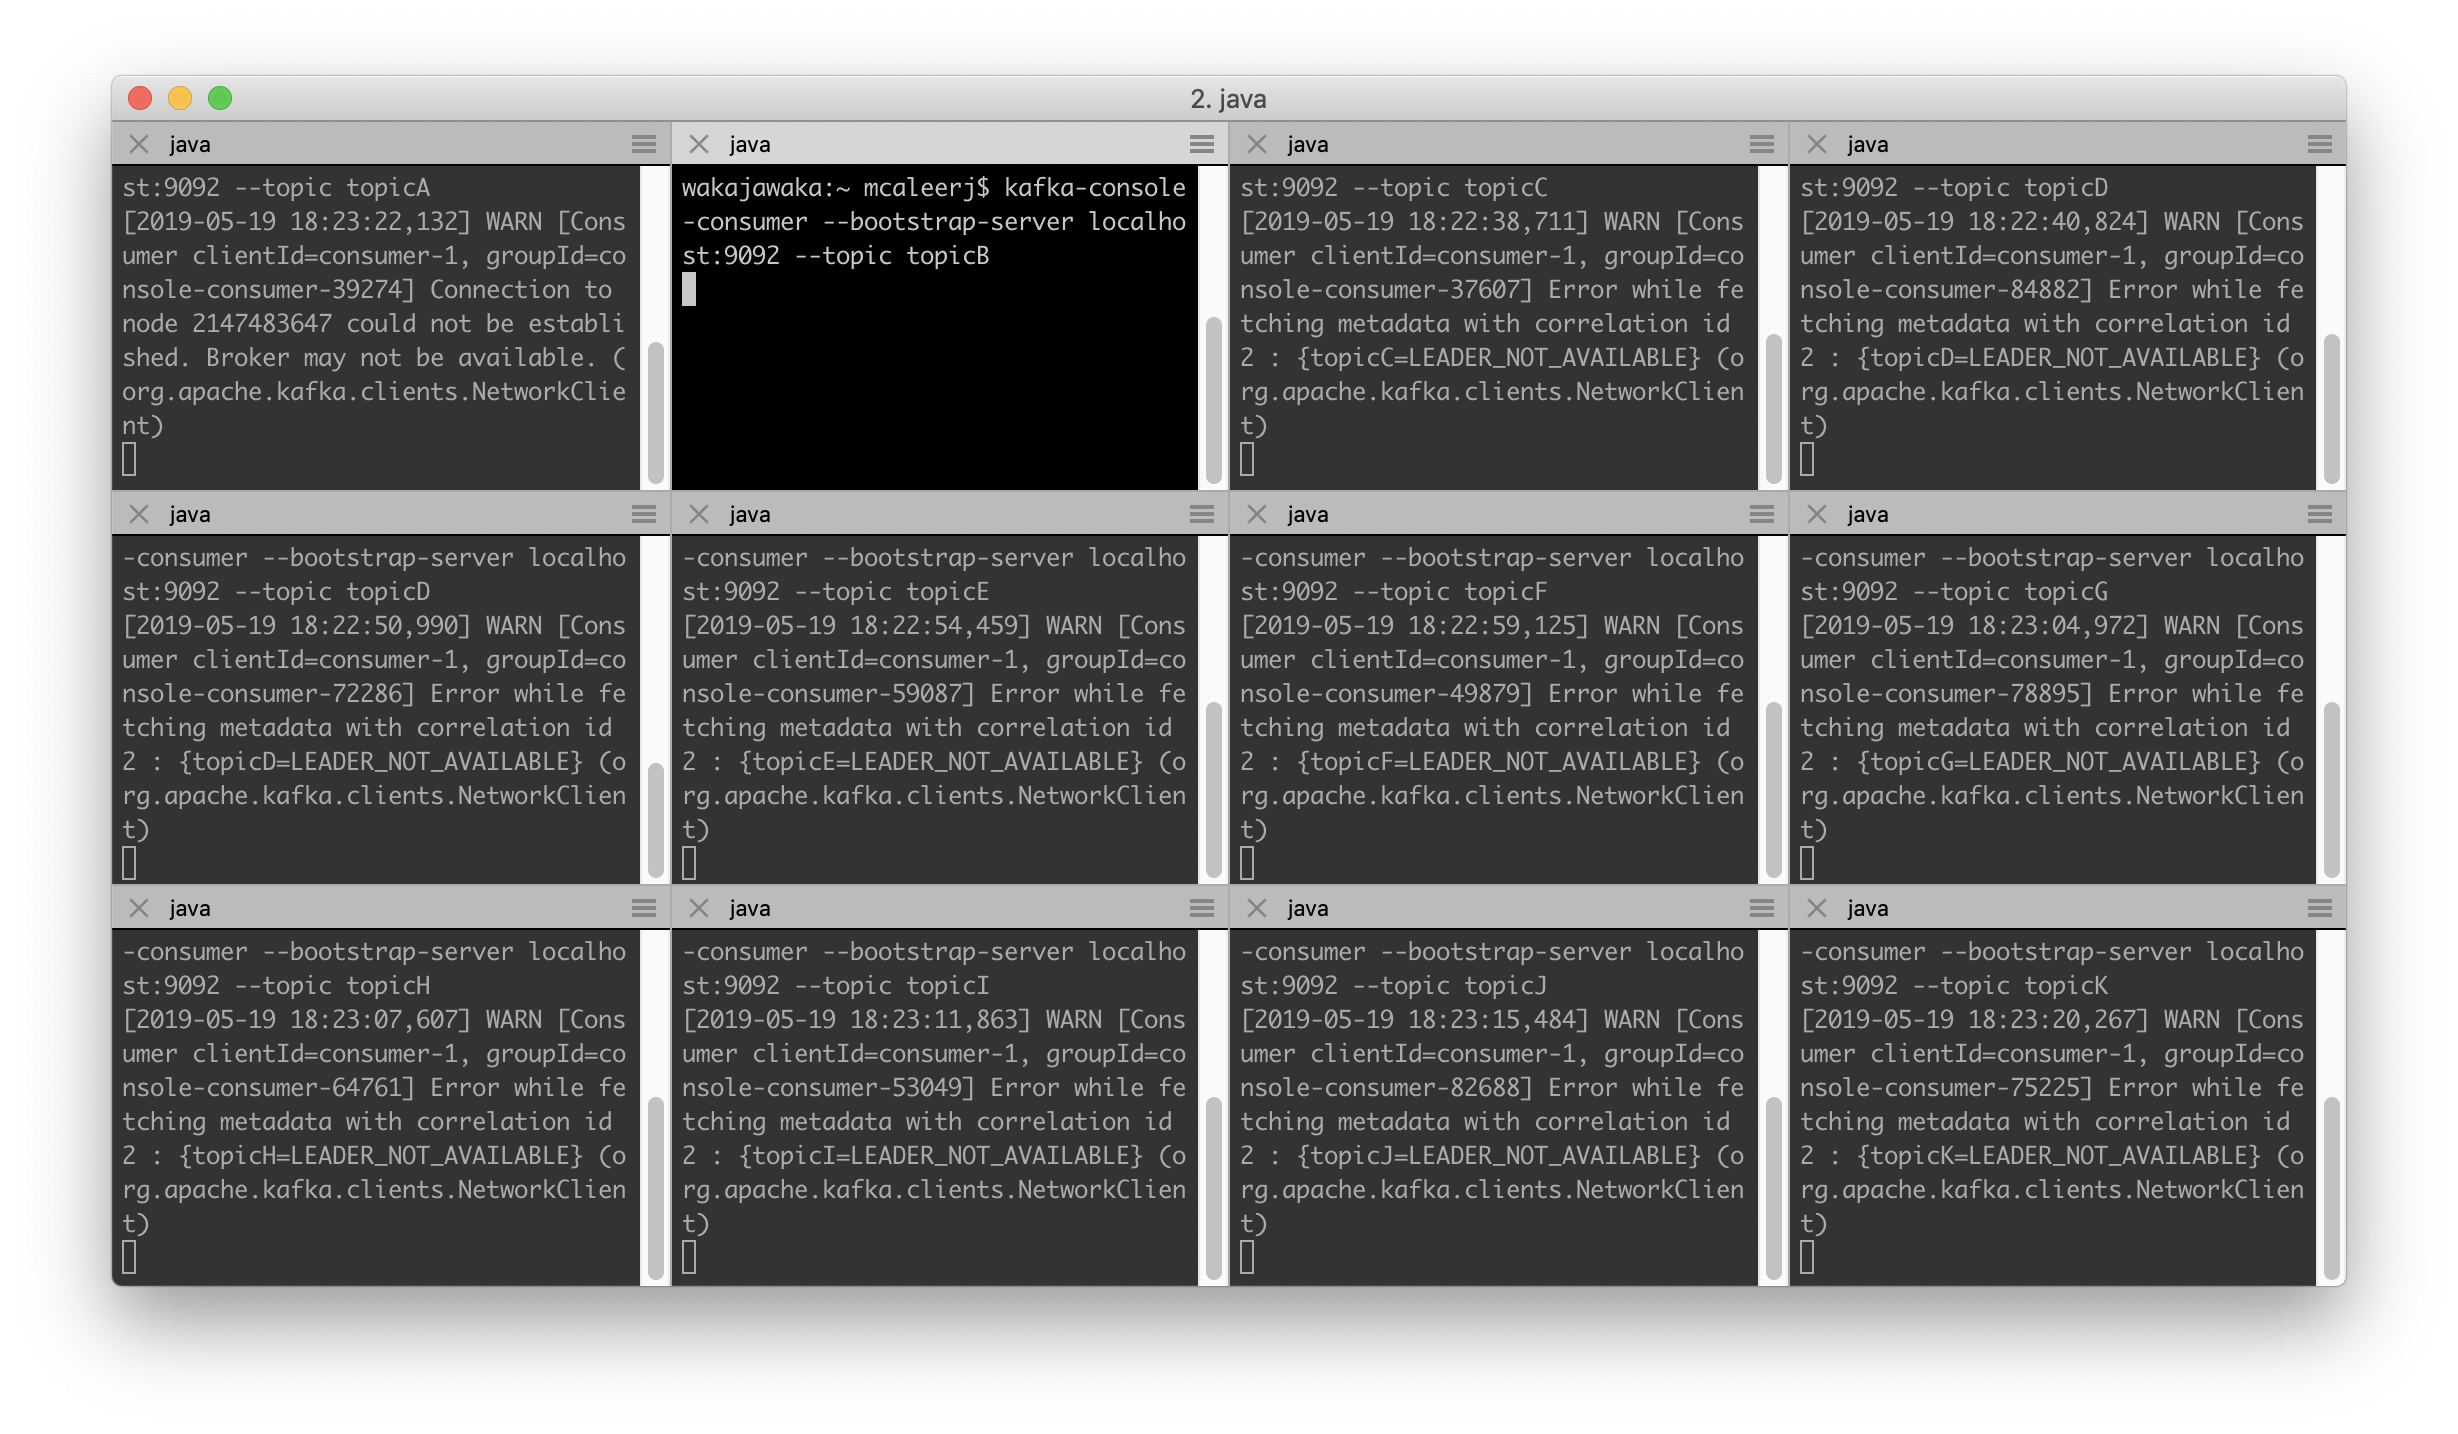
\includegraphics[scale=0.3]{figures/background/monitoring.png}
	\caption{Numerous consoles listening on Kafka topics.}
	\label{console_monitoring}
\end{figure}

With the growth of big data and related disciplines, data pipelines have become an increasingly popular design paradigm; consequently various real-time pipeline monitoring solutions have become available in recent years. Likewise major cloud service vendors now offer a variety of message-driven data pipeline frameworks and accompanying monitoring solutions. In this section, several open-source and proprietary monitoring products will be discussed and compared with the approach and solution proposed by this thesis. 

\subsection{Amazon CloudWatch}
Amazon Managed Streaming for Kafka (Amazon MSK) - is Amazon's managed, Kafka-based service for processing of continuous data streams\cite{AmazonMS34:online}. The offering is currently in its infancy and at time of writing, in public preview. Amazon's corresponding monitoring solution is \textit{Amazon CloudWatch}, which enables collection of metrics such as messages per unit time sent by message producers, the number of network packets transmitted per unit time, log sizes, CPU usage, and the like. As such, Amazon CloudWatch provides no topology discovery functionality whatsoever, and while it collates various metrics at the network and message broker level, does not provide dashboards which convey at a high level, messaging activity across a pipeline. The CloudWatch dashboard interface depicted in Figure \ref{cloudwatch_ui} demonstrates the metrics-focused nature of the solution.

\vspace{5mm}

\begin{figure}[H]
	\centering  
	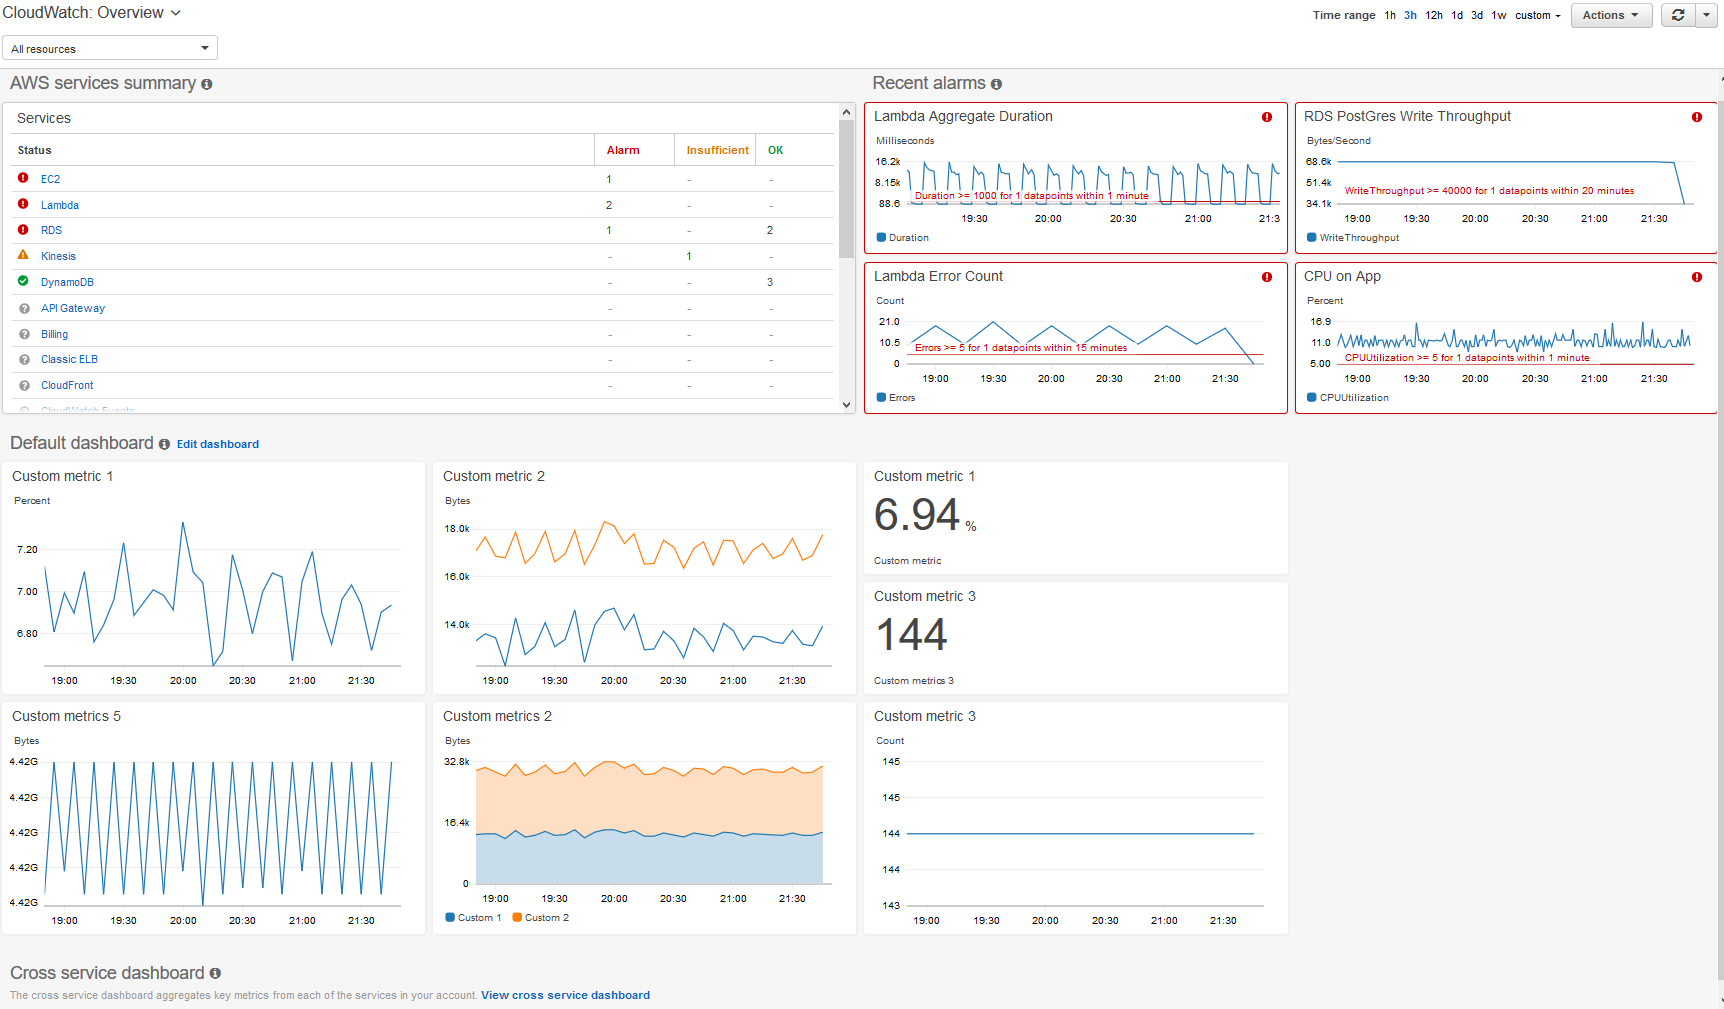
\includegraphics[scale=0.4]{figures/background/cloudwatch.png}
	\caption{Amazon CloudWatch monitoring dashboard.}
	\label{cloudwatch_ui}
\end{figure}

\subsection{Azure Dashboards}
Microsoft's current offerings around implementation of data pipelines are \textit{HDInsight},  \textit{Stream Analytics}, and  \textit{Data Factory}, which variously support implementation of Kafka-based applications, data transformation pipelines, and event processing engines in general. Microsoft enable the creation of monitoring dashboards within the Azure portal; such dashboards can be configured to leverage metrics around pipeline availability and overall pipeline health. The metrics made available correspond to those exposed by Amazon's monitoring solution; CPU usage, network usage, message broker statistics and the like. This metric-centric monitoring solution, like Amazon's \textit{CloudWatch} service, has scarce potential to address the central use case of the solution proposed by this thesis, namely: \textit{As a developer, I want to understand the composition and activity state of my deployed pipeline applications at a glance}. 

Pipeline monitoring solutions offered by the larger cloud players such as Amazon and Microsoft clearly target an Enterprise IT Operations Management (ITOM) audience, concerned primarily with \textit{five nines} availability and application performance. A number of commercial and open-source monitoring solutions focused on topology discovery and pipeline activity monitoring have however emerged in recent years.

\subsection{Lightbend OpsClarity}
\textit{OpsClarity} is a commercial, closed-source software product positioned specifically for real-time data pipeline monitoring\cite{OpsClarity}. OpsClarity reports on a plethora of real-time metrics including pipeline throughput, latency, error rates and data loss.  This solution integrates with a number of popular frameworks including Apache Kafka, Apache Zookeeper, Apache Spark, MongoDB, and Docker. In addition to reporting various pipeline metrics, OpsClarity features automated topology discovery and real-time visualisation for various supported technologies - features which mirror the cornerstone goals of this research. While specific details of how activity monitoring topology discovery is performed are not made available by the product vendor, product documentation does state that discovery and monitoring functionality is implemented by a series of agents \cite{OpsClarity_agents}. Agent installation is required per monitored host. While the monitoring solution proposed in this thesis will likewise be agent and plug-in based, as proposed in Section \ref{exec_summary}, it will not by contrast require configuration or instrumentation of monitored host environments.

In further contrast with the monitoring software proposed by this research, the OpsClarity solution performs activity monitoring at a higher level of granularity. OpsClarity monitors traffic flow between high-level components such as Kafka clusters, Apache Spark engines, Memcache instances, and ElasticSearch instances. While the range of metrics generated by the software is comprehensive, it does not perform topology discovery for microservices communicating within a messaging cluster. This is a key distinction between OpsClarity's offering and the work proposed in this thesis; the prototype developed as part of this dissertation will monitor and reflect messaging activity and pipeline topology \textit{within} for instance a Kafka cluster. The OpsClarity solution regards a Kafka cluster as an atomic entity, communicating with other components of a distributed data pipeline, such a CEP engines, database systems and distributed caches. In continuing contrast, the OpsClarity solution does not provide real-time dashboard visualisation of message aggregation data between pipeline microservices. 

As such, the intended target audience of this offering is an ITOM audience; OpsClarity is not positioned to satisfy the use case stated in the introductory chapter of this thesis, i.e. \textit{As a developer, I want to understand the composition and activity state of my deployed pipeline applications at a glance}.

\subsection{Apache StreamSets}

\textit{StreamSets} is an open source, Apache-licensed framework used for the design, execution and real-time monitoring of data pipelines. Pipeline design an an integral aspect of StreamSets, which features an advanced drag-and-drop UI for pipeline topology design, as depicted in Figure \ref{streamsets_design_ui}. 

\vspace{5mm}

\begin{figure}[H]
	\centering  
	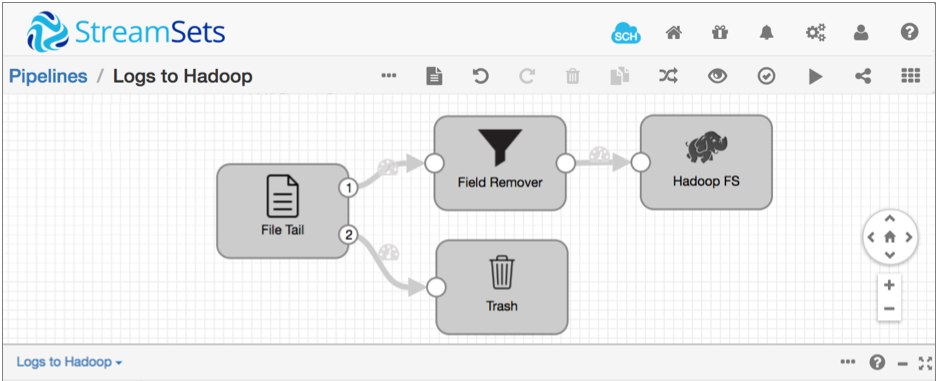
\includegraphics[scale=2.0]{figures/background/streamsets_design_ui.png}
	\caption{StreamSets pipeline topology designer.}
	\label{streamsets_design_ui}
\end{figure}

In contrast with the monitoring solution proposed in this thesis, StreamSets is an encompassing solution, targeting all phases of pipeline lifecycle from design to implementation and monitoring. StreamSets does not feature any form of topology discovery, as pipeline structure is input during the topology design phase of pipeline life-cycle. Moreover, in stark contrast to the proposed monitoring solution, StreamSets cannot be used to monitor a pipeline implemented \textit{without} use of the framework. 

The StreamSets monitoring user interface does not display metrics per message channel or topic, nor does it render channel or topic names; a directed graph representation denotes the sender and consumer of messages only. As such, the monitoring functionality may have limited use as a general-purpose environment monitoring dashboard when framed in the context of questions enumerated in Section \ref{intro_motivation}. The user interface is relatively dense and given the proliferation of controls presented in Figure \ref{streamsets_monitor_ui}, clearly intended for interactive use. Once again revisiting the key use case stated in the introductory chapter - \textit {As a developer, I want to understand the composition and activity state of my deployed pipeline applications at a glance} - StreamSets, while evidently a powerful and popular framework\cite{StreamSe68:online}, does not meet this requirement.

\vspace{5mm}
 
\begin{figure}[H]
	\centering  
	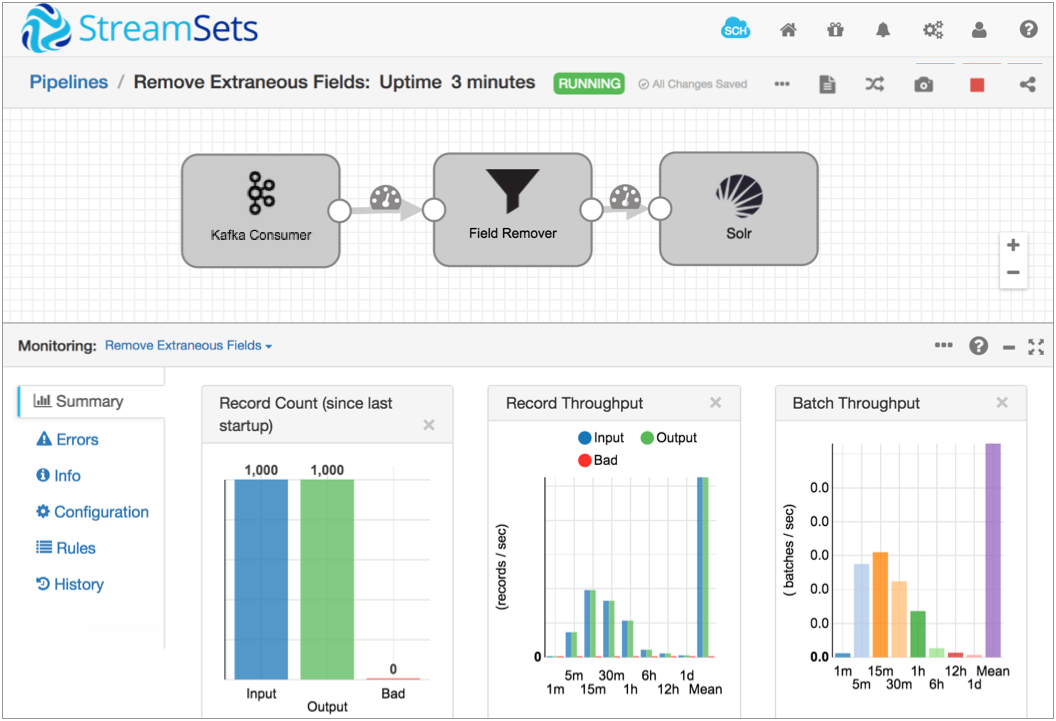
\includegraphics[scale=1.4]{figures/background/streamsets_monitor_ui.png}
	\caption{StreamSets real-time monitoring UI.}
	\label{streamsets_monitor_ui}
\end{figure}

\subsection{Kiali}

\textit{Kiali}, a GitHub-hosted open-source project (https://github.com/kiali/kiali), aims to provide answers to the question: What microservices are part of my Istio service mesh and how are they connected\cite{kiali_online}? Kiali delivers real-time interactive graphs of microservice interactions via interrogation of an \textit{Istio Service Mesh}. Istio documentation defines a service mesh as "\textit{... the network of microservices that make up such applications and the interactions between them}"\cite{Istio_mesh_online}. Istio essentially augments a set of microservices by directing all microservice inter-communication though per-service \textit{sidecars}, intelligent proxies responsible for traffic mediation. A separate Istio \textit{control plane} manages load balancing, routing rules, rate limiters, metric generation and security functionality\cite{Istio_mesh_online}.

Kiali performs pipeline topology discovery and activity monitoring via interrogation of the Istio control plane. Directed graphs are used to render mesh topologies as depicted in Figure \ref{kiali_monitor_ui}; the solution provides inter-service traffic visualisation by animating the edges connecting graph nodes. While this approach achieves the major goals outlined in this research - namely, real-time monitoring and rendition of both data pipeline topology and message activity - pipeline integration with Istio is a prerequisite, which may prohibit use in some environments. Furthermore, the Istio dependency inherently implies a transitive dependency to Kubernetes - prohibiting use of this monitoring solution in alternate environments. While comparatively limited in scope - Kiali enables monitoring of various inter-service communication media - the solution presented in this dissertation is technology-agnostic and considerably more lightweight.

\begin{figure}[H]
	\centering  
	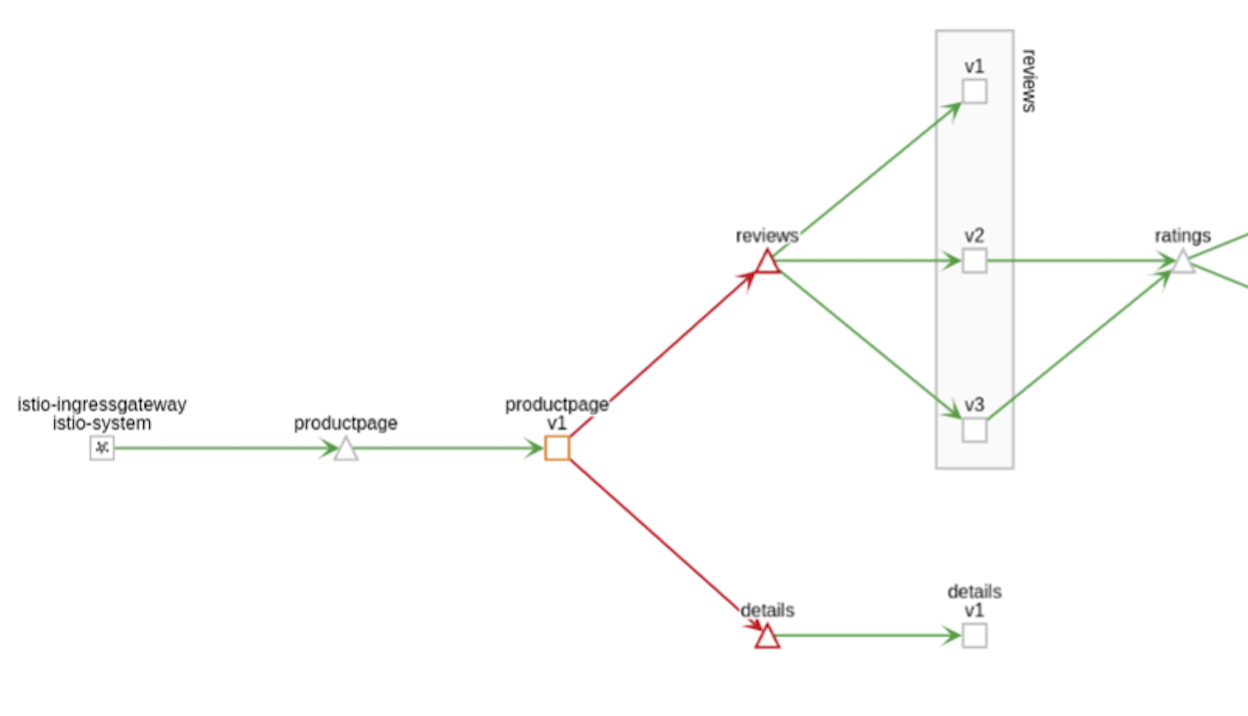
\includegraphics[scale=1.4]{figures/background/kiali.png}
	\caption{Kiali real-time monitoring UI.}
	\label{kiali_monitor_ui}
\end{figure}

In summary, of the real-time pipeline monitoring solutions discussed above, Kiali is alone in featuring both real-time topology discovery and per-message channel activity reporting. As such, of the existing software explored here, it is the only viable successor to the array of console windows depicted in Figure \ref{console_monitoring}.

To contrast Kiali against the solution described by this thesis, the proposed implementation will have relatively few dependencies; monitoring of a Kafka-based pipeline should for instance require details of the Kafka bootstrap server address only. Kiali meanwhile requires full Istio and Kubernetes integration for pipeline deployments. The solution proposed here will be further differentiated by its use of a simple, focused dashboard which clearly communicates information satisfying the basic use case started in the opening chapter. As that use case states, the use case actor in question is not in an ITOM role, but is more likely a software developer or tester. 
 % Introduction

\chapter{Requirements and Design}
\lhead{\emph{Requirements and Design}}

\section{Project Requirements}\label{project_requirements}

Functional and non-functional requirements for the solution implementation are given in the following sections \cite{Sommerville}. The requirements specification leverages terminology defined by RFC2119, \textit{Key words for use in RFCs to Indicate Requirement Levels}.

\subsection{Functional Requirements}

\begin{enumerate}
	\item \textit{(FR-1)} The software MUST support real-time rendering of message activity in a given environment.
	\item \textit{(FR-2)} The software MUST support aggregation of message activity statistics.
	\item \textit{(FR-3)} The software MUST support discovery of environment topology information.
	\item \textit{(FR-4)} The software MUST support rendering of monitored application pipeline topology structures.
	\item \textit{(FR-5)} The software MUST support parallel monitoring and discovery of multiple environments.
	\item \textit{(FR-6)} The software MUST provide an interface for user-configuration of multiple monitored environments.
	\item \textit{(FR-7)} The software MUST support a configurable retention period for monitored environment data.
\end{enumerate}

\subsection{Non-functional Requirements}
\begin{enumerate}
	\item \textit{(NFR-1)}The software MUST be extensible, supporting the addition of additional pipeline discovery and message monitoring implementations with minimal impact.
	\item \textit{(NFR-2)} The software implementation MUST be sufficiently generic to enable monitoring for environments based on disparate messaging technologies, i.e. it MUST NOT be limited to support for a single technology such as Apache Kafka.
\end{enumerate}

\section{Key Concepts and Terminology}

The following key concepts and terminology will be used for the remainder of this document.

\subsection{Environment}

An \textit{environment} is a single running instance of message-driven pipeline application comprising some number of services or microservices which communicate over a messaging system such as Apache Kafka or RabbitMQ. A \textit{monitored} environment is an environment whose topology and message activity are actively observed by the monitoring application.

\subsection{Topology}

Every environment has exactly one associated topology. A topology is either empty or represented as a directed graph, which consisting of a non-empty finite set elements called \textit{nodes} and a finite set of ordered pairs of distinct vertices called \textit{edges}\cite{GraphTheory}. A topology node corresponds to service or consumer/producer of messages in a given environment; every node has an unique associated \textit{name}. A topology edge corresponds to a message \textit{topic} in a message-driven environment; every topology edge has an associate, non-unique \textit{label}. Such a graph is depicted in Figure \ref{topology_graph}.

\begin{figure}[H]
	\centering  
	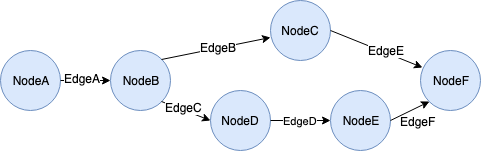
\includegraphics[scale=0.8]{figures/design/topology_graph.png}
	\caption{Example topology graph.}
	\label{topology_graph}
\end{figure}

\section{Architecture Design}

A prototype Monitoring Application will be developed. The software architecture employed will be microservices-based, as this architectural style presents certain advantages in terms of scalability, ease of development, and flexibility.

Functional requirement \textit{(FR-5)} mandates that the Monitoring Application must be capable of monitoring multiple environments simultaneously. Persistence and aggregation of monitored message activity over several environments may require significant processing and storage resources, particularly when monitoring environments containing high volumes of message activity. The horizontal scalability conferred by a microservices architecture is desirable in this case.

It is anticipated that use of a microservices architecture will afford several key advantages during development of the prototype. The inherent decoupling of responsibilities across prototype microservices will allow focused development on isolated aspects of overall application functionality. During development and testing, the ability to redeploy and debug individual services without impacting on all application functionality and availability is expected to reduce both development time and overall complexity. 

In terms of flexibility, the use of co-operating microservices communicating over HTTP enables freedom of choice in terms of language and technology choices per microservice implementation.
Five key functional areas have been identified based on the functional and non-functional requirements as presented. These are:

\begin{enumerate}
	\item Management and persistence of environment configuration and metadata.
	\item Monitoring of environment messaging activity.
	\item Aggregation of environment messaging activity.
	\item Correlation of environment messages based on some criteria.
	\item Real-time rendition of environment topology and message activity information.
\end{enumerate}

The above functional items will be implemented by the microservices enumerated in the following sections.


\subsection{Management Service}

The Management Service will be implemented as a microservice exposing a single external HTTP endpoint. The HTTP endpoint will provide a user-interface for system configuration management, in accordance with requirement \textit{FR-6}. The service will have responsibility for persistence of  application configuration, enabling user registration of monitored environment details. Per-environment discovered topology information will be also managed by this service. Data structures used to represent environment and topology state will be technology-agnostic as required by non-functional requirement \textit{NFR2}.

\subsection{Discovery Service}

The Discovery Service will be implemented as a microservice. The service will be responsible for discovery of environment topology information, in accordance with functional requirement \textit{FR-3}. The implementation will include a Discovery Agent API, which may be implemented for various topology discovery strategies. Agent implementations will be responsible for determining the topology of a given message-driven application environment. The service will be capable of discovering multiple environment topologies concurrently, in accordance with functional requirement \textit{FR-5}. To satisfy requirements \textit{NFR-1 }and \textit{NFR-2}, monitoring functionality will be pluggable, extensible and user-configurable. The Discovery Service will determine the set of monitored environments via interrogation of the Management Service.

\subsection{Monitoring Service}
The Monitoring Service, which will be implemented as a microservice, will be responsible for ingestion and persistence of messages from one or more monitored environments. Monitored message activity will be persisted on receipt, with a configurable retention period configured appropriate for real-time rendition of cluster state. The service will be capable of monitoring multiple environments concurrently, in accordance with functional requirement \textit{FR-5}. To satisfy requirements \textit{NFR-1 }and \textit{NFR-2}, monitoring functionality will be pluggable, extensible and user-configurable.

\subsection{Aggregation Service}
The Aggregation Service will be implemented as a microservice, having responsibility for real-time generation of environment summary information. Collated environment information including environment metadata and categorised message counts  per unit time will be pushed asynchronously to clients in accordance with functional requirement \textit{FR-1}. The service will be capable of aggregating data for multiple environments in parallel, in accordance with functional requirement \textit{FR-5}. The Aggregation Service will determine the set of monitored environments via interrogation of the Management Service.

\subsection{Correlation Service}
The Correlation	 Service will be implemented as a microservice, having responsibility for generation of message correlation information on monitored environments. It will expose a HTTP-based client interface.

\subsection{API Gateway}

Use of an API Gateway service is a common pattern in microservice architecture applications. It will provide a single point of access to backend services for client applications such as the Dashboard Client, masking application partitioning details.

\subsection{Client Dashboard / UI Service}

The Client Dashboard will render environment state for consumption by end-users in accordance with function requirement \textit{FR-1}. Dashboard updates - which include environment topology and environment state summary change notifications - will be pushed to the Dashboard application asynchronously.

\subsection{Service Registry}

Use of a Service Registry is a common pattern in microservice architecture applications. The registry will allow inter-service communication without the need for hard-coded host / port information.

Figure \ref{arch_high_level} depicts the overall application architecture (the UI Service and Service Registry have been omitted from this diagram).

\vspace{5mm}


\begin{figure}[H]
	\centering  
	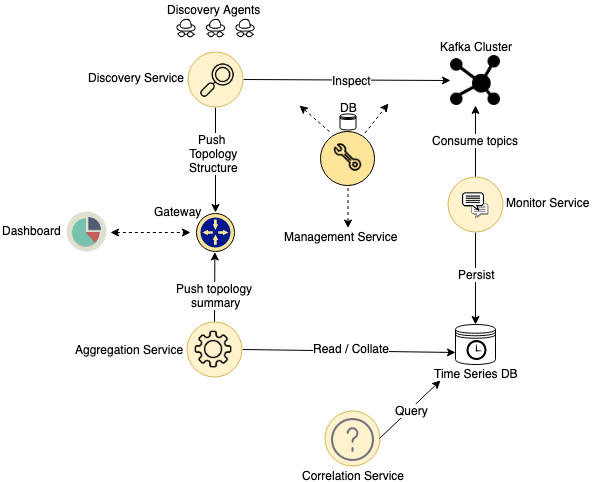
\includegraphics[width=\linewidth]{figures/design/arch_high_level.png}
	\caption{Software architecture high-level design.}
	\label{arch_high_level}
\end{figure}

\section{Design Scope}

Non-functional requirement \textit{NFR-2} mandates that the solution implementation must be sufficiently generic and extensible to support multiple messaging technologies. Plug-in interfaces will enable the implementation and addition of technology-specific discovery and monitoring implementations. For purposes of this dissertation, the author has chosen to focus on plug-in and agent implementations for a single messaging framework, namely Apache Kafka (hereafter referred to simply as Kafka)\cite{ApacheKafka}. The motivation for this choice is professional exposure to Kafka-based message processing pipelines, coupled with the contemporary ubiquity of the framework.

Kafka is an open source messaging and stream processing platform, whose key concepts include  \textit{topics}, \textit{producers} and \textit{consumers}. As the nomenclature implies, consumers and producers consume and produce Kafka messages respectively. Messages are associated with a specific, named \textit{topic}; producers and consumers may produce to and consume from multiple topics. The example topology depicted in Figure \ref{topology_graph} corresponds to a Kafka-based application as described in \ref{topology_to_kafka_mapping}.

\vspace{10 mm}

\begin{table}[H]
	\centering
	\begin{tabular}{ |p{4cm}||p{8cm}| }
		\hline
		Topology Object & Kafka Object \\
		\hline
		\textbf{NodeA}   & Producer application NodeA   \\
		\textbf{EdgeA}   & Message topic named EdgeA   \\
		\textbf{NodeB}   & Producer/consumer application NodeB   \\
		\textbf{EdgeF}   & Message topic named EdgeF   \\
		\textbf{NodeF}   & Consumer application NodeF   \\	    
		\hline
	\end{tabular}
	\caption{Topology to Kafka mapping.}
	\label{topology_to_kafka_mapping}
\end{table}

Kafka enjoys broad client language support, and as such Kafka-based environments may include applications built using Java, C/C++, Python, JavaScript, Erlang and numerous other languages. For purposes of this dissertation the author will focus on Java-based environments.

The challenges inherent to the design of functional topology discovery and monitoring plug-in implementations for a Kafka and Java based environment will be explored in the following sections.

\section{Design Challenges - Edge Correlation}

Assuming the availability of a topology model for a given environment, the following are requirements for successful monitoring and rendition of messaging activity in the environment:

\begin{enumerate}
	\item All messages generated in the monitored environment must be accessible to the monitoring application.
	\item For a given message, the monitoring application must be capable of correlating the message to a  topology edge.
\end{enumerate}

In order to successfully correlate a message to a graph edge, the monitoring application must be capable of determining the graph node responsible for production of the message. Consider the topology depicted in Figure \ref{topology_unique_edge_labels}. All edges in this topology have unique labels; thus, on observation of a Kafka message on topic \textbf{EdgeA}, it is possible to correlate that message with a single graph edge.

\begin{figure}[H]
	\centering  
	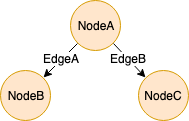
\includegraphics[scale=0.8]{figures/design/topology_unique_edges.png}
	\caption{Topology of unique edge labels.}
	\label{topology_unique_edge_labels}
\end{figure}

Now, consider the topology depicted in Figure. \ref{topology_non_unique_edge_labels}. Topolgy edge labels are non-unique; in this example, graph edges \textit{(NodeD, NodeB)} and\textit{(NodeC, NodeD)} share the edge label \textbf{EdgeC}. In order to successfully correlated a monitored message with a single topology edge, the first element of the ordered pair must be known.

\vspace{5mm}

\begin{figure}[H]
	\centering  
	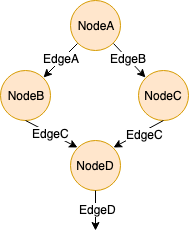
\includegraphics[scale=0.8]{figures/design/topology_non_unique_edges.png}
	\caption{Topology of non-unique edge labels.}
	\label{topology_non_unique_edge_labels}
\end{figure}

Thus, for a monitored Kafka environment in which multiple producers generate messages on a given topic, the monitoring application must determine the sender of a given message in order to successfully render message activity in the environment.

Kafka messages do not, however, identify the message sender. Figure \ref{kafka_consumer_record_api} describes the Java API for Kafka ConsumerRecord, which defines the interface to messages read by a Kafka consumer.

\begin{figure}[H]
	\centering  
	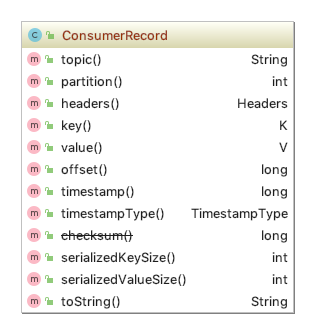
\includegraphics[scale=2.5]{figures/design/consumer_record_api.png}
	\caption{Kafka Consumer Record Java API.}
	\label{kafka_consumer_record_api}
\end{figure}

While the consumer of a message can determine the message topic, timestamp and value amongst other fields, there is no information pertaining to the producer of the message. Not only does the Kafka API not yield this information; the underlying Kafka protocol for message delivery to consumers contains no fields describing a message sender.  The protocol defines the message record structure as follows\cite{KafkaProtocol}:

\vspace{5mm}

\begin{lstlisting}[caption={Kafka Protol Message Record Definition},captionpos=b]
Record =>
Length => varint
Attributes => int8
TimestampDelta => varint
OffsetDelta => varint
KeyLen => varint
Key => data
ValueLen => varint
Value => data
Headers => [Header]

Header => HeaderKey HeaderVal
HeaderKeyLen => varint
HeaderKey => string
HeaderValueLen => varint
HeaderValue => data
\end{lstlisting}

The absence of producer information in the protocol message structure rules out approaches such as packet inspection or bytecode manipulation as a means of determining the producer of a message. 

Kafka headers have been identified as a suitable means to augment messages in order to convey producer information to message consumers. Kafka documentation describes headers as "... an API for metadata information to be added to kafka messages and a way for plugins and interceptors to add, remove, modify and otherwise act based on this metadata"\cite{KafkaHeaders}.

By augmenting all produced messages with a known header denoting the source node name, the monitoring application can successfully identify same during message consumption. Several approaches to header addition have been explored.

\subsection{Manual Header Injection} \label{manual_header_addition}

A straightforward approach to Kafka header injection involves manually updating application code to add the designated source node header to any message sent by a monitored service. The following code demonstrates the sending of a message in a Spring Boot application:

\vspace{5mm}

\begin{lstlisting}[language = Java, caption={Sending a message with Spring Kafka},captionpos=b]
public void sendMessage(final String messageData) {
Message<String> message = MessageBuilder
.withPayload(data)
.build();
template.send(message);
}
\end{lstlisting}

To add the appropriate header and value to the produced message, the code should be updated as follows, where \textit{SOURCE\_NODE\_ID} is a header name known to the monitoring environment, and \textit{APPLICATION\_NAME}, the header value, provides the unique name of the application.

\vspace{5mm}

\begin{lstlisting}[language = Java, caption={Sending a message with Spring Kafka},captionpos=b]
public void sendMessage(final String messageData) {
Message<String> message = MessageBuilder
.withPayload(data)
.setHeader(SOURCE_NODE_ID_HEADER, APPLICATION_NAME)
.build();
template.send(message);
}
\end{lstlisting}

This solution is however highly undesirable for several reasons:

\begin{enumerate}
	\item The approach is particularly invasive, requiring potentially widespread updates to producer source code. 
	\item Developers are likely to overlook the need for header addition when implementing new message producers.
	\item Ideally application source code should not have dependencies on or knowledge of any monitoring environment. 
\end{enumerate}

While this approach is undesirable, it is nonetheless an option when a less invasive means of header injection is impossible, as may be the case for Kafka producers implemented in languages such as C.

\subsection{Log Analysis}

For environments that leverage distributing tracing solutions such as Spring Cloud Sleuth, log analysis may be used to derive the sender of a given message. This approach has been evaluated in the context of Spring Boot applications. Crucially, Spring/Kafka integration code will log the production of every message before sending; the logging operation is performed by the class \texttt{org.springframework.kafka.core.KafkaTemplate}. At time of writing, the latest Spring Kafka versions will log the following information per message:

\begin{itemize}
	\item The topic name.
	\item The message key and value.
	\item The message timestamp.
\end{itemize}

Log analysis pseudocode is presented in Listing \ref{log_analysis_pseudocode}.

\begin{lstlisting}[caption={Log analysis pseudocode},captionpos=b,label={log_analysis_pseudocode}]
def getProducer(message):
for entry in log_entries:
if(entry.topic == message.topic &&
entry.timestamp == message.timestamp &&
entry.key == message.key &&
entry.value == message.value):
return entry.application_name
return NULL
\end{lstlisting}

While this approach is far less invasive than that described in Section \ref{manual_header_addition}, requiring no modifications to application source code, it does require a number of conditions to be true:

\begin{itemize}
	\item Appropriate logging levels must be set for all monitored applications.
	\item Distributed logging must be enabled.
	\item Logging configuration must include logging of the application name.
	\item Collated logs must be made available to the monitoring application (via a solution such as Logstash(Kibana).
\end{itemize}

This approach suffers from a number of limitations which impact on its feasibility; Spring Boot's logging behaviour is not guaranteed in any way and may change between releases, thus rendering log information useless. The time required to perform log analysis - as a function of log collection and scanning time - may have an adverse affect as regards real-time rendition of environment state as mandated by functional requirement \textit{(FR-1)}. Furthermore, this approach may not be applicable at all with alternate implementations such as Kafka for Python, Kafka for Node.js and others.

Finally and critically; if multiple producers dispatch identical messages to a given topic at the same instant in time - however unlikely this is - log analysis will be unable to collate the messages to a topology graph edge. 

\subsection{Header Injection via Application Framework Hooks} \label{kafka_producer_header_design}

Application frameworks may provide hooks and extension points which can be leveraged from the perspective of modifying application behaviour in a transparent and non-invasive fashion. The Spring framework provides one such hook in the form of the \textit{BeanPostProcessor}. This interface "\textit{...allows for custom modification of new bean instances, e.g. checking for marker interfaces or wrapping them with proxies.}"\cite{BeanPostProcessor}. Figure \ref{spring_bean_lifecycle} describes the various phases involved in initialisation of a Spring bean.

\vspace{5mm}

\begin{figure}[H]
	\centering  
	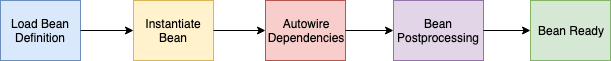
\includegraphics[scale=0.6]{figures/design/beanpostprocessor.png}
	\caption{Spring bean initialisation.}
	\label{spring_bean_lifecycle}
\end{figure}

The bean post-processing phase of bean initialisation affords an opportunity to perform customisation on Spring beans, including those involved in dispatching of Kafka message in Spring applications. One such bean type is the Spring framwork class \texttt{org.springframework.integration.channel.AbstractMessageChannel}. This abstract bean type provides methods for configuration of \texttt{ChannelInterceptor}s, documented as ".\textit{..(an) interface for interceptors that are able to view and/or modify the Messages being sent-to and/or received-from a MessageChannel}"\cite{ChannelInterceptor}.

By leveraging Spring Auto-Configuration\cite{SpringFactories} in combination with a custom bean post-processor, message headers denoting the message producer name can be transparently injected into all messages produced by a given application. Enabling this behaviour is as simple as adding an application runtime dependency to the injection library. This strategy has several advantages:

\begin{itemize}
	\item The method is minimally invasive - no modifications to source code are required.
	\item Developers of new producers are not concerned with addition of custom headers.
	\item Message consumers such as the environment monitor application can determine the sender of message with guaranteed accuracy, minimal processing time, and minimal dependencies.
\end{itemize}

This approach, if successful, will be the preferred implementation for edge correlation functionality detailed in Section \ref{software_impl_producer_ident}.

\section{Design Challenges - Topology Discovery} \label{design_topology_discovery}

\subsection{Manual Topography Configuration} \label{}

If an environment cannot be automatically discovered or only partially discovered by automated discovery agents, users of the monitoring application will require functionality enabling manual topography configuration. To this end, the Management Service will provide a client interface which enables viewing and management of environment topographies.

The topology graph depicted in Figure \ref{topology_non_unique_edge_labels} might be described by the  proposed JSON structure given in Listing \ref{topology_JSON}. A corresponding topology definition format will be defined; this format will be consumed and produced at the Management service client interface.

\vspace{5mm}

\begin{lstlisting}[caption={Sample JSON topology structure.},captionpos=b,label={topology_JSON}]
{
"nodes":[ 
{
"name": "NodeA"
},
{
"name": "NodeB"
},
{
"name": "NodeC"
},
{
"name": "NodeD"
}
],
"edges": [
{
"label": "EdgeA",
"source": "NodeA",
"target": "NodeB"
},
{
"label": "EdgeB",
"source": "NodeA",
"target": "NodeC"
},
{
"label": "EdgeC",
"source": "NodeB",
"target": "NodeD"
},
{
"label": "EdgeC",
"source": "NodeC",
"target": "NodeD"
}           
]
}
\end{lstlisting}


\subsection{Kubernetes Discovery Agent}\label{design_kubernetes_discovery_agent}

Environment topology structure may be determined from metadata extant in application deployment environments such as Kubernetes. A \textit{Kubernetes Discovery Agent} will be implemented in order to explore and demonstrate this approach.  Kubernetes (https://kubernetes.io/) is a popular open-source container orchestration system, used for management of automated application deployment and scaling. Kubernetes supports an application configuration mechanism called a \textit{ConfigMap}, a means of externalising and decoupling application configuration from application implementation and packaging, in a manner that allows the configured application to remain agnostic of the fact that it is executing in a manager Kubernetes environment.

An example Kubernetes ConfigMap is presented in Listing \ref{k8s_configmap_sample}. 

\begin{lstlisting}[caption={Kubernetes ConfigMap sample},captionpos=b,label={k8s_configmap_sample}]

kind: ConfigMap
apiVersion: v1

metadata:
name: myMicroservice-example-config
namespace: myPipeline

data:
property.key.a: propertyValue
property.key.b: propertyValue

\end{lstlisting}

Additional properties can be added to ConfigMaps at any time - including application runtime - without impacting on running applications. By adding known properties to a ConfigMap such as the example given in Listing \ref{k8s_configmap_sample}, metadata describing a subset of an application's topology graph artefacts can be made available for interrogation by third parties such as a Discovery Agent. Listing \ref{k8s_configmap_topolofy_metadata_sample} details an example of such metadata. The listed metadata describes \textbf{NodeB} and adjacent edges as given in the topology sample rendered in Figure \ref{topology_non_unique_edge_labels}.  In this proposed scheme, a topology node name is denoted by property \texttt{mon.agent.nodename} while incoming and outgoing edges are described by properties \texttt{mon.agent.incoming-edges }and \texttt{mon.agent.outgoing-edges} respectively.

\vspace{5mm}

\begin{lstlisting}[caption={Kubernetes ConfigMap containing topology metadata},captionpos=b,label={k8s_configmap_topolofy_metadata_sample}]

kind: ConfigMap
apiVersion: v1

metadata:
name: myMicroservice-example-config
namespace: myPipeline

data:
mon.agent.nodename: NodeB
mon.agent.incoming-edges: EdgeA
mon.agent.outoing-edges: EdgeC

property.key.a: propertyValue
property.key.b: propertyValue

\end{lstlisting}

The Kubernetes/Kafka Discovery Agent will be configured with the details of the Kubernetes cluster in which a given monitored application is running. Thereafter it will iteratively discover topology information using the algorithm presented by the pseudocode in Listing \ref{k8s_kafka_agent_pseudeocode}.

\vspace{5mm}

\begin{lstlisting}[caption={Kubernetes/Kafka Discovery Agent Algorithm},captionpos=b,label={k8s_kafka_agent_pseudeocode}]

for environment in monitoredEnvironments:

let topology = new Topology()

for configMap in kubernetes_namespace:
if isDiscoverable(configMap):
let nodeName = configMap.nodeName
let incomingEdges = []
let outgoingEdges = []
for topicName in configMap.consumed_topic_list:
incomingEdges.append(topicName)
for topicName in configMap.consumed_topic_list:
outgoingEdges.append(topicName)

topology.addNode(nodeName):
for(edge in incomingEdges)
topology.addEdge(edge)
for(edge in outgoingEdges):
topology.addEdge(edge)	

environment.merge(topology)
\end{lstlisting}

This approach to dynamic discovery of application topologies in Kubernetes environments  is not bound to any specific messaging technology or language implementation.

\subsection{Message Correlation Agent}\label{design_message_correlation}

In the absence of topology metadata, topology structure can nonetheless be deduced for a subset of topology structures. By correlation of related messages observed in a monitored environment a set $\theta$ of related messages may be observed. By placing a temporal ordering upon messages in the set $\theta$, it is possible to deduce the set of nodes and ordered edges that comprise a given topology. 

When related environment messages contain shared Universally Unique Identifiers (UUIDs), the set  $\theta$ is constructed trivially, by identification of observed messages with a common UUID value. While more challenging approaches to message correlation may be necessary depending on payload structures present in monitored environments, the aforementioned approach of simple field-matching correlation will be employed in the development of the monitoring application prototype.

To this end, the Correlation Service will support the implementation of a correlation-based Discovery Agent. This Agent will periodically request correlation traces from the Correlation Service; returned trace information will then be used to determine partial topology structure. 

The Correlation Service will perform correlation by determining the set of unique monitored values for a given payload field in a given environment during a moving temporal window. For each unique field value found, the service will determine the set of matching messages, ordering these by message timestamp. The service will return such traces to clients via a client interface, returning a JSON structure such as the following:

\begin{lstlisting}[caption={Correlation Service Message Trace}]
{
"messages": [
{
"edgeLabel": "edgeB",
"sourceNode": "nodeA",
"timestamp": {
"time": 1557419028600
}
},
{
"edgeLabel": "edgeC",
"sourceNode": "nodeB",
"timestamp": {
"time": 1557419028597
}
},    
{
"edgeLabel": "EdgeD",
"sourceNode": "nodeD",
"timestamp": {
"time": 1557419028602
}
}
]
}

\end{lstlisting}

Certain topology structures / monitored environments cannot be accurately discovered using this approach. Such topologies include:

\begin{itemize}
	\item Topologies in a which a single message received on a given node results in multiple messages traversing fan-out edges of the same node. In such topologies, a temporally ordered set of messages does not yield the order in which nodes are traversed.
	\item Topologies in which sink nodes do not contain fan-out edges. As messages are never observed as originating from such nodes, correlation traces processed by the correlation Discovery Agent will not contain messages indicating the existence of such a node. Similarly, any edge on which a message is never produced cannot be discovered using this approach; entire subgraphs will remain undiscovered in this circumstance.
	\item Environments in which message production time (as opposed to monitoring/consumption time) cannot be determined.  
	
\end{itemize}


\subsection{Static Code Analysis}

Static code analysis tools may be used to determine the topology of a given environment given the availability of source code for the various microservices comprising same. Common software implementation patterns may be exploited in order to determine the set of incoming and outgoing edges for a given topology node. 

In the case of Java-based Spring Boot application, consumer and producer message streams are typically configured using custom \textit{channel annotations}, which declare the existence of uniquely named message streams. An example is given in the following Java code snippet.

\vspace{5mm}

\begin{lstlisting}[caption={Spring Boot Cloud Channel Annotations}]
@Input("my.input.channel")
SubscribableChannel inboundMessages();   

@Output("my.output.channel")
MessageChannel validatedMessages();
\end{lstlisting}

Input and output channels are further configured for specific message technology using \textit{stream bindings}. For a Spring Boot microservice leveraging Apache Kafka, the input and output streams given in the previous code example might be bound as demonstrated by the following YAML snippet:

\vspace{5mm}

\begin{lstlisting}[caption={Spring Boot Cloud Channel Binding Configuration}]
spring:
cloud:
stream:
kafka:
bindings:
my.input.channel:
destination: source
contentType: application/json
my.output.channel:
destination: validated
contentType: application/json
\end{lstlisting}

Such code and configuration may be statically analysed in order to extract the set of input and output channels defined by a Spring application; by parsing the sources to all pipeline microservices, a topology structure can be derived. While this approach will not be explored any further during the development of the monitoring application, the following skeletal prototype demonstrates that static discovery of input and output channels for a Spring Boot application is not a complex task. The following code leverages the open source \textit{JavaParser} library available at https://github.com/javaparser/javaparser. Complete sources are bundled with monitoring application at \newline https://github.com/schmigware/monitoring-app.

\vspace{5mm}

\begin{lstlisting}[caption={Discovery of Spring Cloud message channels by static analysis}]
package org.cit.mcaleerj.thesis.analysis.sample;

import com.github.javaparser.JavaParser;
import com.github.javaparser.ast.body.MethodDeclaration;
import com.github.javaparser.ast.expr.AnnotationExpr;
import com.github.javaparser.ast.visitor.VoidVisitorAdapter;

import java.io.File;
import java.io.IOException;

import java.util.Optional;

public class FindStreamAnnotationSample {

public static void findStreamAnnotations(final File projectDir) {
final ProjectExplorer exp = new ProjectExplorer(new AnnotationProcessor());
exp.process(projectDir);
}

private static class AnnotationProcessor implements ProjectExplorer.FileProcessor {

public void process(final File file) {

try {
new VoidVisitorAdapter<Object>() {
@Override
public void visit(final MethodDeclaration decl, final Object arg) {
super.visit(decl, arg);
Optional<AnnotationExpr> optional = decl.getAnnotationByClass(
org.springframework.cloud.stream.annotation.Input.class);
optional.ifPresent(annotation -> {
processStreamInputAnnotation(annotation);
});
optional = decl.getAnnotationByClass(
org.springframework.cloud.stream.annotation.Output.class);
optional.ifPresent(annotation -> {
processStreamOutputAnnotation(annotation);
});
}
}.visit(JavaParser.parse(file), null);

} catch (IOException e) {
new RuntimeException(e);
}
}

private void processStreamInputAnnotation(final AnnotationExpr exp) {
//process input annotation
}

private void processStreamOutputAnnotation(final AnnotationExpr exp) {
//process input annotation
}

}

}

\end{lstlisting}

\section{Design Challenges - Topology Visualisation}\label{design_topology_visualisation}

In order to satisfy requirements \textit{FR-1} and \textit{FR-4}, the topology visualisation implementation should provide the following:

\begin{enumerate}
	\item Rendition of the most up-to-date topology structure for a monitored environment.
	\item Rendition of real-time message activity information for topology edges.
	\item Rendition of supplementary information such as environment name and edge activity snapshot time.
\end{enumerate}

A browser-based \textit{Client Dashboard} will be implemented to satisfy the above requirements. The Dashboard will render a information pertaining to a single monitored environment, using the layout proposed in Figure \ref{dashboard_high_level}. Environment name and snapshot time will convey the to users information about which environment is currently rendered, and the time at which message activity was observed. The topology itself - which is modelled internally as a digraph by the monitoring application - will likewise be rendered as a directed graph at the dashboard.

\begin{figure}[H]
	\centering  
	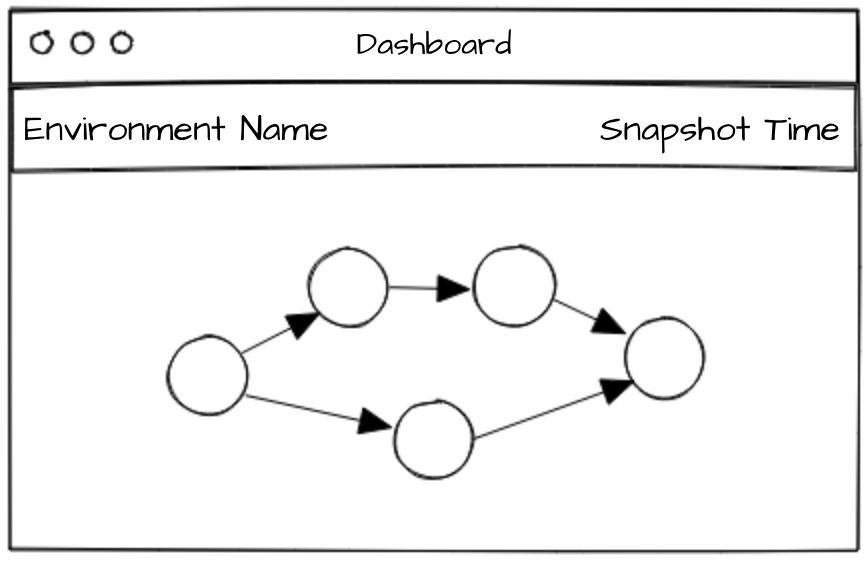
\includegraphics[scale=0.8]{figures/design/viz_high_level.png}
	\caption{High Level Client Dashboard Layout}
	\label{dashboard_high_level}
\end{figure}

\subsection{Graph Node Visualisation}\label{design_client_dashboard}

The topology graph will comprise three classes of node. Each node will be rendered using a visually distinct style.

\begin{enumerate}
	\item \textit{Topology nodes}. Such nodes correspond to discovered services (message consumers/producers) in a monitored environment. Topology nodes will be rendered using a simple, uniform and coloured geometric shape which includes the discovered node name. A proposed rendering style is demonstrated in Figure \ref{dashboard_node_high_level}.
	
	\begin{figure}[H]
		\centering  
		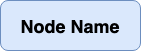
\includegraphics[scale=0.8]{figures/design/dashboard_node_high_level.png}
		\caption{Proposed Topology Node visualisation.}
		\label{dashboard_node_high_level}
	\end{figure}
	
	
	\item \textit{Source nodes}. A Source Node is added to the graph for every graph edge which has no discovered topology node as its discovered source node. Such an edge might represent incoming messages from an external system. No node label is rendered for such nodes, which will be rendered using an identifiable, uniquely styled geometric shape such as that proposed in Figure  \ref{dashboard_source_node_high_level}.
	
	\begin{figure}[H]
		\centering  
		
\includegraphics[scale=0.8]{figures/design/dashboard_source_node_high_level.png}
		\caption{Proposed Source Node visualisation.}
		\label{dashboard_source_node_high_level}
	\end{figure}
	
	\item \textit{Sink nodes}. A Sink Node is added to the graph for every graph edge which has no discovered topology node as its target node. Such an edge might represent messages outgoing to an external system.  No node label is rendered for such nodes, which will be rendered using an identifiable, uniquely styled geometric shape such as that proposed in Figure  \ref{dashboard_sink_node_high_level}.
	
	\begin{figure}[H]
		\centering  
		
\includegraphics{figures/design/dashboard_sink_node_high_level.png}
		\caption{Proposed Sink Node visualisation.}
		\label{dashboard_sink_node_high_level}
	\end{figure}
\end{enumerate}

\subsection{Graph Edge Visualisation}
Graph edges will be rendered using directed arrows. Each edge will be labelled with:

\begin{itemize}
	\item  The associated edge name, corresponding to for instance a message topic name in a monitored Kafka environment.
	\item An activity summary, displaying the number of messages monitored per second on the given edge. 
\end{itemize}

The proposed rendition for a topology edge is depicted in Figure \ref{dashboard_edge_high_level}.
\vspace{5mm}

\begin{figure}[H]
	\centering  
	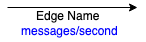
\includegraphics{figures/design/dashboard_edge_high_level.png}
	\caption{Proposed Edge visualisation.}
	\label{dashboard_edge_high_level}
\end{figure}

\subsection{Rendering Real-Time Topology Structure and Activity}

Monitored environment topology discovery and activity aggregation will be performed on an ongoing and real-time basis by various backend services. The Client Dashboard will subscribe to these services for asynchronous notifications pertaining to topology structure changes and edge activity information. Such information will be rendered on receipt by the client. 

\section{Software Development Methodology}\label{design_methodology}

The Waterfall model\cite{Palmquist13parallelworlds} will be employed during development of the monitoring prototype. Given the solution will be implemented as a set of microservices, the methodology will be applied in an iterative fashion. Initially, the contracts between co-operating microservices will be identified. Thereafter, the Waterfall model will be applied to the implementation of each service in turn. The order in which the various components will be implemented is expected to flow as follows, respecting the dependencies between services.

\begin{enumerate}
	\item Service Registry 
	\item Management Service
	\item Monitoring Service
	\item Monitoring task implementation(s)
	\item Aggregation Service
	\item Correlation Service
	\item Discovery Service
	\item Discovery Agent implementation(s)
	\item Gateway Service
	\item UI Service / Dashboard Client
\end{enumerate}

It is anticipated that some retrospective design and implementation revision will be necessarily undertaken during development of the solution.

Successful implementation of the solution will depend on application of an existing software development skill-set and knowledge base, which will be augmented by developing a working knowledge of several technologies including:

\begin{itemize}
	\item Spring Boot 2.0
	\item D3 Visualisation Framework  
	\item WebSocket API
	\item GraphQL API
	\item Kubernetes / Minikube
\end{itemize}

\section{Software Evaluation}\label{design_evaluation}

The success of the software prototype will be evaluated in term of the use case set out in the opening chapter of this thesis: 

\textit {As a developer, I want to understand the composition and activity state of my deployed pipeline applications at a glance}.


 % Requirements and Design

\chapter{Software Implementation}
\lhead{\emph{Software Implementation}}

The following key technologies have been chosen for implementation of the Monitoring Application prototype.

\begin{itemize}
	
	\item \textbf{Java} version 8 (https://www.java.com) has been selected as the implementation language for prototype microservices, as the author has considerable experience with same.
	
	\item \textbf{Python} has been chosen as the implementation language for any command-line tooling developed as part of the prototype's supporting ecosystem.
		
	\item \textbf{Spring Boot} (https://spring.io/projects/spring-boot) is a popular, Java based application framework designed around the principle of convention-over-configuration \cite{Conventi95:online}. Spring Boot provides a powerful data access framework as well as out-of-the-box integration with popular messaging frameworks such as Kafka and RabbitMQ. Features such as integrated job scheduling and service discovery are key to the rapid development of several required application features. As an experienced Java developer, choice of this framework will minimise ramp-up time for the author. Spring Boot will underpin all microservices comprising this prototype.
	
	\item \textbf{Kafka} client for Java (https://kafka.apache.org). While the monitoring application prototype will be implemented in a technology-agnostic fashion in accordance with requirement  \textit{(NFR-2)}, plug-ins providing Kafka monitoring will be implemented using Kafka client libraries.
		
	\item \textbf{GraphQL} (https://graphql.org), developed by Facebook \cite{GraphQLA36:online}, has been chosen as the HTTP service interface implementation technology for all microservices providing same. An alternative to REST, GraphQL presents only a single client endpoint per service, supporting the query and mutation of service data. GraphQL servers present clients with schema metadata which allows for the development of powerful and intuitive client tools such as Insomnia IDE \cite{GraphQLI51:online}.
	
	\item \textbf{PostgreSQL} database (https://www.postgresql.org) has been chosen as the underlying persistence technology for the monitoring application. PostgreSQL's native support for persistence and querying of JSON data is a clear choice for persistence of monitored environment message payloads.
	
	\item The \textbf{WebSocket API} \cite{TheWebSo73:online}, part of the HTML5 specification, provides persistent full-duplex communication between centlient browsers and web servers. Asynchronous notifications will be pushed from Monitoring Application microservices to the Dashboard Client using this technology.
	
	\item \textbf{Dagre-d3} (https://github.com/dagrejs/dagre-d3) is a JavaScript library used to display directed graphs in web browsers. Based on the popular and powerful \textbf{D3} (https://d3js.org/) visualisation library,Dagre-d3 will underpin the Client Dashboard implementation.
	,
\end{itemize}

Additionally, \textbf{Kubernetes}, \textbf{Minikube},  \textbf{Kafka} and  \textbf{Zookeeper} will be extensively used in development of a test bed application, as described in Appendix A.

Implementation details for the various prototype microservices are explored in the following sections.

\section{Management Service}

This microservice is responsible for management and persistence of environment and topology state. An embedded web server hosting a GraphQL service provides a client interface for both users of the software and cooperating microservices, satisfying function requirement \textit{FR-6}. Users leverage the GraphQL interface to define and manage environment profile, environment, and topology information. Likewise, microservices such as the Aggregation and Discovery services communicate with the Management Service in order to enumerate monitored environment details and populate topography data. This microservice is implemented as a Spring Boot application, with a dependency on PostgreSQL database.

\subsection{Domain Model} \label{management_service_domain_model}
The domain model underpinning the Management Service has been designed with flexibility in mind. Environment configuration and topology models are sufficiently abstract to describe the properties of a pipeline application, without specific bindings to for example, Kafka related concepts. The data model underlying the Management Service is depicted in Figure \ref{mgmt_svc_domain_model}.

 \begin{figure}[H]
	\centering  
	\includegraphics[height=0.6\textheight]{figures/impl/mgmt/domain_package.png}
	\caption{Management Service data model.}
	\label{mgmt_svc_domain_model}
\end{figure}


The \textbf{Environment} model is the central type implemented by the Management Service. It models a single monitored environment, for example a Kafka-based pipeline application instance. An Environment comprises:
\begin{itemize}
	\item A unique name and UUID.
	\item A flag which indicates whether the environment is actively monitored.
	\item Exactly one associated \textbf{EnvironmentProfile}.
	\item Some number of associated \textbf{Configuration Properties}.
\end{itemize}

The \textbf{EnvironmentProfile} model specifies configuration information for a given class of environment, for example a Kafka or RabbitMQ-based application environment. Extending the Configurable model, the EnvironmentProfile specifies configuration properties which are read by various clients of the Management Service; the qualified class names of environment-specific monitoring task implementations are for instance provided as part of EnvironmentProfile. Additional attributes of the EnvironmentProfile are:
\begin{itemize}
	\item A unique profile identifier.
	\item An informational profile name.
\end{itemize}

An Environment may have at most one associated \textbf{Topology} instance. A Topology models a \textit{directed graph}, comprising one or more \textbf{Nodes}. A Node may have zero or more incoming and outgoing \textbf{Edges}. Every node has a name attribute, which is unique per topology. Every edge has a label attribute; multiple edges can share a common label.

A simplified example of the domain model for a given environment is given in Figure \ref{mgmt_svc_domain_model_example}. In this example, an EnvironmentProfile with profileId \textbf{KAFKA} has been defined. The profile defines a single configuration property named  \textbf{monitoringClass}. A single Environment is associated with this profile; the environment is named  \textbf{MyKafkaApp}, and is configured such that monitoring is enabled. A single configuration property, \textbf{bootstrap-server}, designates the host and port at which the environment's Kafka bootstrap server can be found. Finally, a simple topology comprising four nodes is associated with the environment.

 \begin{figure}[H]
	\centering  
	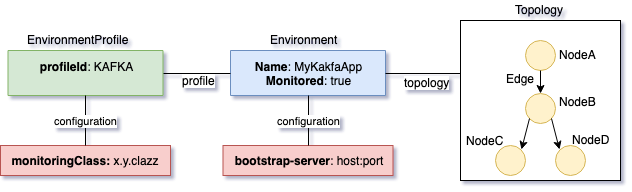
\includegraphics[width=\linewidth]{figures/impl/mgmt/mgmt_domain_example.png}
	\caption{Management Service simplified domain example.}
	\label{mgmt_svc_domain_model_example}
\end{figure}

\subsection{Modules}
The Management Service comprises the modules depicted in  \ref{mgmt_svc_modules}. The structure is typical of a Spring Boot based microservice.

\begin{figure}[H]
	\centering  
	\includegraphics[width=\linewidth]{figures/impl/mgmt/modules.png}
	\caption{Management Service modules.}
	\label{mgmt_svc_modules}
\end{figure}

\subsection{Component Interactions}
The Management Service presents a single external interface, detailed in the following sections. This interface provides various CRUD operations on Environments, EnvironmentProfiles, and Topology models. A GraphQL \textit {CommandResolver} implements the external interface. It in turn invokes a \texttt{ManagementService} interface, which further interacts with a JPA-based persistent model repository. The simple sequence diagram presented in Figure  \ref{mgmt_svc_seq_diagram} exemplifies the component interactions involved in enabling monitoring for a given environment.

 \begin{figure}[H]
	\centering  
	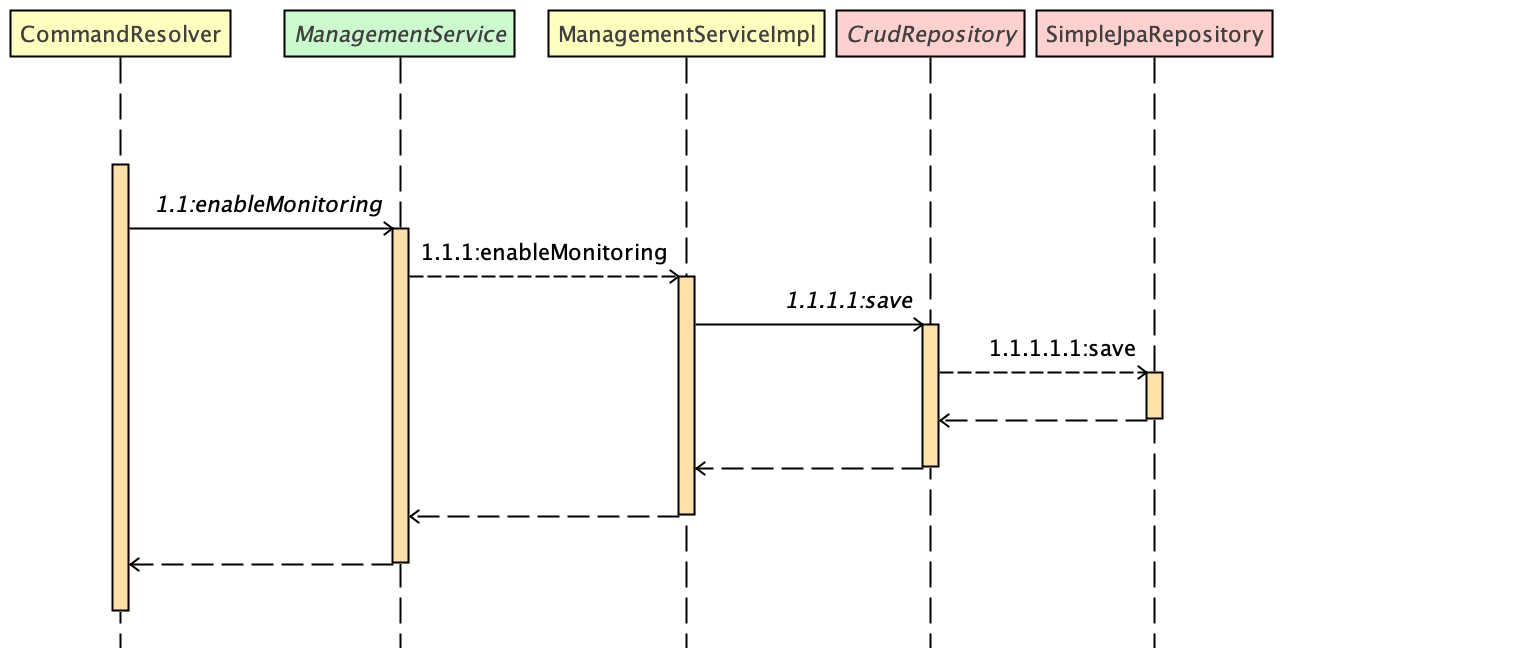
\includegraphics[width=\linewidth]{figures/impl/mgmt/enable_monitoring_seq.png}
	\caption{Sequence diagram: Enabling monitoring for an environment.}
	\label{mgmt_svc_seq_diagram}
\end{figure}

\subsection{External Interface} \label{management_service_external_interfaces}

The Management Service implements a GraphQL interface, providing CRUD operations across EnvironmentProfile, Environment, and Topology models. Both end users and other microservices are clients of this interface. End users are expected to interact directly with the GraphQL endpoint using suitable tooling. 

The Management Service implements a client module intended for import by other services; it abstracts the GraphQL interface, provided simple programmatic access to the service. Table \ref{mgmt_svc_graphql_operations} lists the various operations supported by the Management Service.

\vspace{10 mm}

\begin{table}[H]
	\centering
	\begin{tabular}{ |p{4cm}||p{4cm}| }
		\hline
		Domain Type& Operations \\
		\hline
		EnvironmentProfile   & register   \\
		& list   \\
		& delete   \\
		&     \\
		Environment &register \\
		&list \\
		&list monitored \\
		&update \\
		&delete \\
		&enable monitoring \\
		&disable monitoring \\
		&     \\
		Topology & register \\
		& list \\
		& update \\
		& delete \\
		\hline
		\end{tabular}
	\caption{Management Service GraphQL operations.}
		\label{mgmt_svc_graphql_operations}
\end{table}

\newpage
 
\section{Monitoring Service}

This microservice is responsible for the persistence of message traffic observed in monitored environments. It depends upon the Management Service for discovery of monitored environment information, synchronising periodically in order to start and stop concurrently executing environment monitoring tasks, partially satisfying functional requirement \textit{FR-5}. The implementation is agnostic of messaging technologies, in accordance with non-functional requirement \textit{NFR-2}. A \textit{MonitoringTask API} provides for the addition of technology-specific monitoring task implementations to this service, satisfying non-functional requirement \textit{NFR-1}; a Kafka-specific implementation has been provided with this prototype. Monitored environment messages are persisted, with a configurable retention period set by default to one hour. Furthermore, the module exports a data access module which is used by co-operating microservices such as the Aggregation Service. This microservice is implemented as a Spring Boot application, with a dependency on PostgreSQL database.

\subsection{Domain Model}
The Monitoring Service implements a simple domain model, comprising a single type \textbf{Message}. A Message represents a single message observed in a monitored environment. It comprises:

\begin{itemize}
	\item The identifier of the environment in which the message was observed.
	\item The edge label. While the Message type is technology agnostic, for a message observed in a Kafka-based environment, this attribute will correspond to a Kafka topic name.
	\item The source node name. In a Kafka-based environment, this attribute designates the message producer.
	\item The message content.
	\item The message timestamp.
\end{itemize}

The data model is depicted in Figure \ref{monitoring_svc_domain_model}.

\vspace{10 mm}

 \begin{figure}[H]
	\centering  
	\includegraphics[scale=1.8] {figures/impl/monitor/domain_package.png}
	\caption{Monitoring Service domain model.}
	\label{monitoring_svc_domain_model}
\end{figure}

\subsection{Modules} \label{monitoring_service_modules}
The Monitoring Service comprises the modules depicted in  \ref{monitoring_svc_modules}. The structure is typical of a Spring Boot based microservice.

\begin{figure}[H]
	\centering  
	\includegraphics[width=\linewidth]{figures/impl/monitor/modules.png}
	\caption{Monitoring Service modules.}
	\label{monitoring_svc_modules}
\end{figure}

\subsection{Component Interactions} \label{monitoring_service_interactions}

The Monitoring Service does not implement any external interfaces. It is driven by a scheduled synchronisation task which executes at a configurable interval, by default every five seconds. The synchronisation task first determines the set of currently monitored environments by polling the Management Service via its client module, as described in section \ref{management_service_external_interfaces}. The component interactions are depicted in Figure \ref{monitoring_sync_task_sequence}.

\begin{figure}[H]
	\centering  
	\includegraphics[width=\linewidth]{figures/impl/monitor/sync_task_seq.png}
	\caption{Monitored Environment synchronisation.}
	\label{monitoring_sync_task_sequence}
\end{figure}

The synchronization task now passes the set of monitored environment definitions to the \texttt{MonitoringService} interface; the implementation creates new monitoring tasks for environments which are not already subject to monitoring, while stopping any redundant monitoring tasks.

A \texttt{MonitoringTask} instance models a single environment monitoring job; an instance of MonitoringTaskFactory in module \textit{monitoring-service-job} dynamically instantiates such tasks via inspection of the \texttt{EnvironmentProfile} associated with a given \texttt{Environment} instance (see section \ref{management_service_domain_model}).

A single concrete implementation of the  \texttt{MonitoringTask} interface has been implemented. This task  implements the functionality required to perform monitoring a Kafka environment. It performs the following  steps in a dedicated monitoring thread:

\begin{itemize}
	\item Determine all known topic names via the Kafka client API.
	\item Create a dedicated monitoring thread.
	\item Create a Kafka consumer for the configured environment, configured to poll indefinitely.
	\item For each incoming Kafka message:
	\begin{itemize}
		\item Create a new \textit{Message} domain object.
		\item Set the message edge label to the name of the topic on which the message was received.
		\item Determine the message source node name via header inspection. The approach used to achieve header injection is described in section \ref{kafka_producer_header_design}.
		\item Set the message content to that of the received Kafka message.
		\item Set the Message timestamp and environment UUID.
		\item Save the message to a persistent JPA repository.
	\end{itemize}
\end{itemize}

\subsection{Monitoring Task API}
To extend the functionality of the software via addition of additional monitoring tasks for various technologies , the \texttt{MonitoringTask} interface must be implemented, and the implementation class(es) made available on the runtime classpath of the Monitoring Service. The service will dynamically instantiate such task implementations based on environment profile configuration as described in section \ref{monitoring_service_interactions}. This simple API provides methods for initialisation of the task with environment information and a \texttt{MessageRepository} instance. Additional methods instruct the monitoring task to start/stop execution.

\begin{figure}[H]
	\centering  
	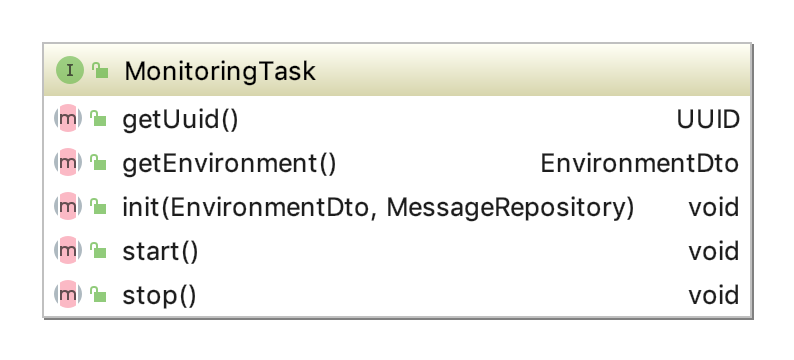
\includegraphics[scale=2.0]{figures/impl/monitor/monitoring_task.png}
	\caption{MonitoringTask API.}
	\label{monitoring_task_api}
\end{figure}


\subsection{Message Repository} \label{monitoring_service_message_repository}
The Monitoring Service defines a DAO module which is used by other microservices (specifically, the Aggregation Service and the Message Correlation Discovery Agent as discussed later in this document) to perform message lookup. This functionality is provided by an implementation of]  a \texttt{MessageRepository} interface, which defines methods for finding all environment messages in a given temporal window, finding the first and last messages for a given environment, finding the next sequential message for a given environment and edge and so on. A generic \texttt{executeQuery} method is provided for clients with esoteric query requirements. The interface class diagram is given in Figure \ref{monitoring_sync_message_repository}.

\begin{figure}[H]
	\centering  
	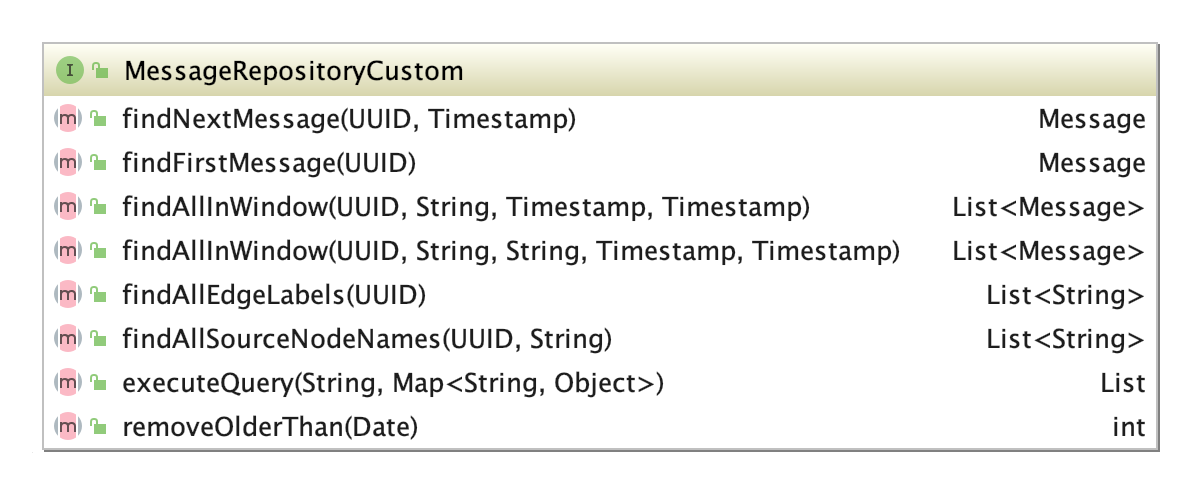
\includegraphics[width=\linewidth]{figures/impl/monitor/message_repository.png}
	\caption{Monitoring Service MessageRepository interface.}
	\label{monitoring_sync_message_repository}
\end{figure}

\subsection{Message Retention} \label{monitoring_service_message_retention}
The \texttt{Purge} module depicted in section \ref{monitoring_service_modules} is responsible for the flushing of persisted messages; the purge operation is performed at a configurable interval, with messages older than a configurable retention period being deleted from persistent storage. This functionality is intended to limit the application's use of disk space. 
\newpage

\section{Aggregation Service}

This microservice is responsible for the aggregation of message traffic persisted by the Monitoring Service, satisfying functional requirement \textit{FR-2}. Furthermore, it is responsible for the near real-time dispatch of aggregation data to interested parties such as the Dashboard Client. Environment aggregations for multiple monitored environments are performed in parallel for a one-second rolling window, implementing functional requirement \textit{FR-5}. Aggregations are persisted, with a configurable retention period set by default to one hour. Asynchronous aggregation notification are pushed to clients using Spring WebSocket support. This microservice is implemented as a Spring Boot application, with a dependency on PostgreSQL database. It leverages a data access module exported by the Monitoring Service for lookup of persisted messages.


\subsection{Domain Model} \label{aggregation_service_domain_model}
The Aggregation Service domain model comprises two models.The first, \texttt{EvironmentAggregation}, models aggregations across all edges for a given environment and temporal window. Every \texttt{EvironmentAggregation} has zero or more associated  \texttt{EdgeAggregation}s, which in turn model the number of messages observed for a given edge label and source node name.

 \begin{figure}[H]
	\centering  
	\includegraphics[scale=3.0] {figures/impl/aggregation/domain_package.png}
	\caption{Aggregation Service domain model.}
	\label{aggregation_svc_domain_model}
\end{figure}

An example of this domain model is given in Figure \ref{aggregation_svc_domain_model_example}. In this example, a single environment aggregation has been performed for a one-second window ending at time 18:09:51. The environment aggregation comprises aggregations for edges \textit{source}, \textit{validated} and \textit{ingest}. 5 messages have been aggregated on each of these edges during the one-second aggregation window.

\begin{figure}[H]
	\centering  
	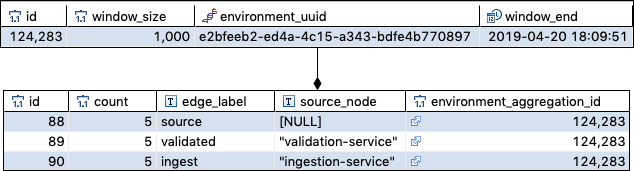
\includegraphics[width=\linewidth]{figures/impl/aggregation/domain_example.png}
	\caption{Aggregation Service domain example.}
	\label{aggregation_svc_domain_model_example}
\end{figure}

\subsection{Modules}\label{aggregation_service_modules}
The Aggregation Service comprises the modules depicted in  \ref{aggregation_svc_modules}. The structure is typical of a Spring Boot based microservice.

\begin{figure}[H]
	\centering  
	\includegraphics[width=\linewidth]{figures/impl/aggregation/modules.png}
	\caption{Aggregation Service modules.}
	\label{aggregation_svc_modules}
\end{figure}

\subsection{Component Interactions}

The Aggregation Service is driven by a scheduled synchronisation task which executes at a configurable interval, by default every five seconds. The synchronisation task first determines the set of currently monitored environments by polling the Management Service via its client module, as described in section \ref{management_service_external_interfaces}. The component interactions are depicted in Figure \ref{aggregation_sync_task_sequence}.

\begin{figure}[H]
	\centering  
	\includegraphics[width=\linewidth]{figures/impl/aggregation/sync_task_seq.png}
	\caption{Monitored Environment synchronisation.}
	\label{aggregation_sync_task_sequence}
\end{figure}

The synchronization task now passes the set of monitored environment definitions to the \texttt{AggregationService} interface; the implementation creates new aggregation tasks for environments which are not already subject to aggregation, while stopping any redundant aggregation tasks.

An \texttt{AggregationTask} instance models a single environment aggregation job; an instance of AggregationTaskFactory in module \textit{aggregation-service-job} is responsible for task instantiation. Each aggregation tasks leverages a MonitoringRepository instance (see Section \ref{monitoring_service_message_repository}) to collate recently monitored messages, aggregating message counts across a configurable aggregation window, which is sized to one second by default.

Each aggregation tasks runs in a dedicated thread, executing on condition that the aggregated environment is configured for monitoring at the Management Service. Aggregation tasks perform an initial check for unaggregated historical messages at task startup; if such messages are discovered, historical aggregation is performed. 

Whenever a new \texttt{EvironmentAggregation} is created, a notification is dispatched to any \texttt{AggregationListener}s registered with the aggregation task. The  \texttt{AggregationListener} is described in section \ref{aggregation_service_notifications}.

\subsection{Aggregation Notifications} \label{aggregation_service_notifications}.
The Aggregation Service implements a single external interface, enabling client registration for asynchronous push notifications of environment-specific aggregation results over the WebSocket protocol \cite{WebSockets}. Clients of the Aggregation Service register for notifications by opening a WebSocket connection to the service instance, specifying the UUID of the environment for which notifications should be dispatched. An \texttt{AggregationServiceMessageHandler} in instantiated per client connection, which in turn registers an \texttt{EnvironmentAggregationListener} with the \texttt{AggregationService}. This listener implementation mediates \texttt{AggregationTask} notifications between the service and registered listeners.

\begin{figure}[H]
	\centering  
	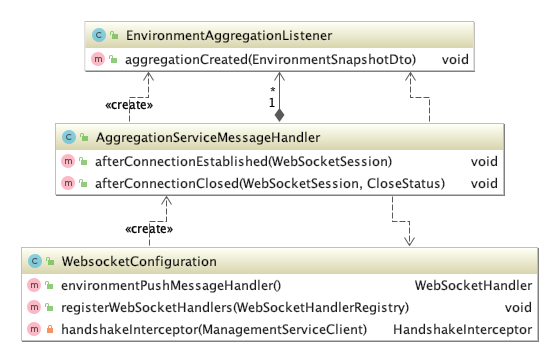
\includegraphics[width=\linewidth]{figures/impl/aggregation/websocket_package.png}
	\caption{Aggregation Service websocket package.}
	\label{aggregation_service_websocket_package}
\end{figure}

Aggregation domain objects are converted to equivalent Data Transfer Objects for dispatch to aggregation listeners. The information ultimately conveyed to listeners is described by Figure \ref{aggregation_service_dto_package}.

\begin{figure}[H]
	\centering  
	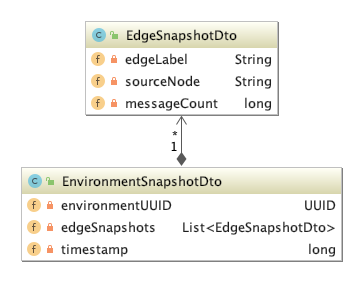
\includegraphics[scale=3.0]{figures/impl/aggregation/dto_package.png}
	\caption{Aggregation Service notification DTOs.}
	\label{aggregation_service_dto_package}
\end{figure}
 
\subsection{Aggregation Retention} \label{aggregation_service_message_retention}
The \texttt{Purge} module depicted in section \ref{aggregation_service_modules} is responsible for the flushing of persisted aggregations; the purge operation is performed at a configurable interval, with aggregations older than a configurable retention period being deleted from persistent storage. This functionality is intended to limit the application's use of disk space. 

\newpage
 
 \section{Correlation Service}
 
This microservice is responsible for the generation of correlation traces for messages observed in monitored environments, as described in section \ref{design_message_correlation}. An embedded web server hosting a GraphQL service provides a client interface for both users of the software and cooperating microservices. In this prototype implementation, the primary function of the Correlation Service is to support the Message Correlation Discovery Agent, discussed in section \ref{discovery_service_correlation_agent}. This microservice is implemented as a Spring Boot application.
 
 \subsection{Domain Model} \label{correlation_service_domain_model}
 The Correlation service domain model comprises three models. The Data Transfer Object pattern is used throughout this service. The first model, \texttt{CorrelationTraceDto}, models a single correlation trace for a monitored environment. It comprises a temporally ordered set of  \texttt{MessageDto} instances, each of which models a correlated message in a given monitored environment. Finally, an instance of  \texttt{CorrelationTraceFilterDto} is passed to the service by clients when requesting a correlation trace;  trace requests are specified by environment UUID and correlated field name. A class diagram is provided in Figure \ref{correlation_svc_domain_model}.
 
 \begin{figure}[H]
 	\centering  
 	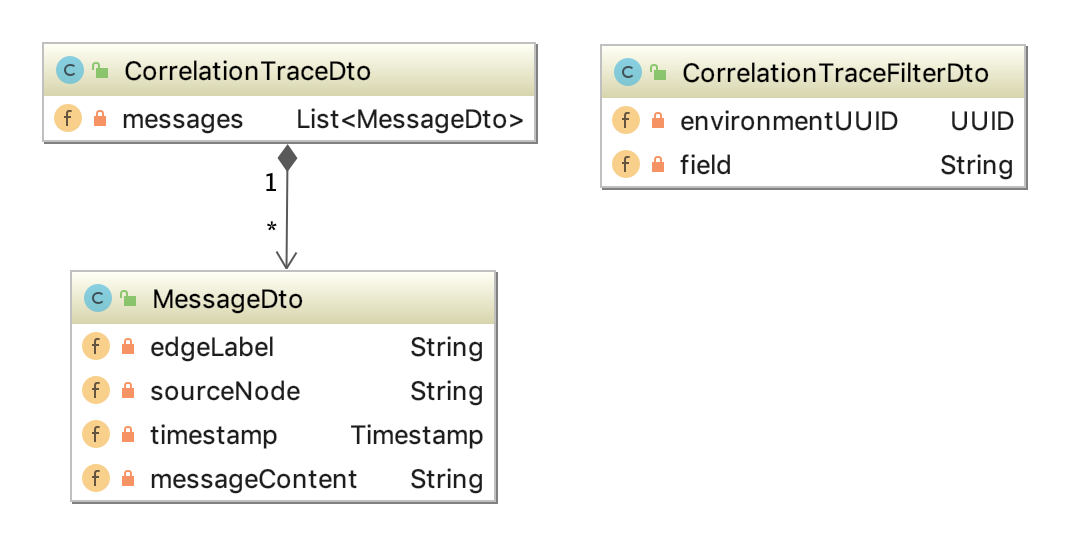
\includegraphics[scale=1.5] {figures/impl/correlation/domain.png}
 	\caption{Correlation Service domain model.}
 	\label{correlation_svc_domain_model}
 \end{figure}
  
 \subsection{Modules}
 The Correlation Service comprises the modules depicted in \ref{correlation_svc_modules}.  The structure is typical of a Spring Boot based microservice.
 
 \begin{figure}[H]
 	\centering  
 	\includegraphics[width=\linewidth]{figures/impl/correlation/modules.png}
 	\caption{Correlation Service modules.}
 	\label{correlation_svc_modules}
 \end{figure}

\subsection{Component Interactions}
The Correlation Service presents a single external interface. This interface provides a single query operation responsible for generation of correlation traces. A GraphQL \textit {CommandResolver} implements the external interface. It in turn invokes a \texttt{CorrelationService} interface, an implementation of which is responsible for trace generation, by querying the monitored message set via a  \texttt{DAO} module imported from the Monitoring Service. The simple sequence diagram presented in Figure  \ref{correlation_svc_seq_diagram} exemplifies the component interactions involved in generation of a correlation trace for a given environment.

\begin{figure}[H]
	\centering  
	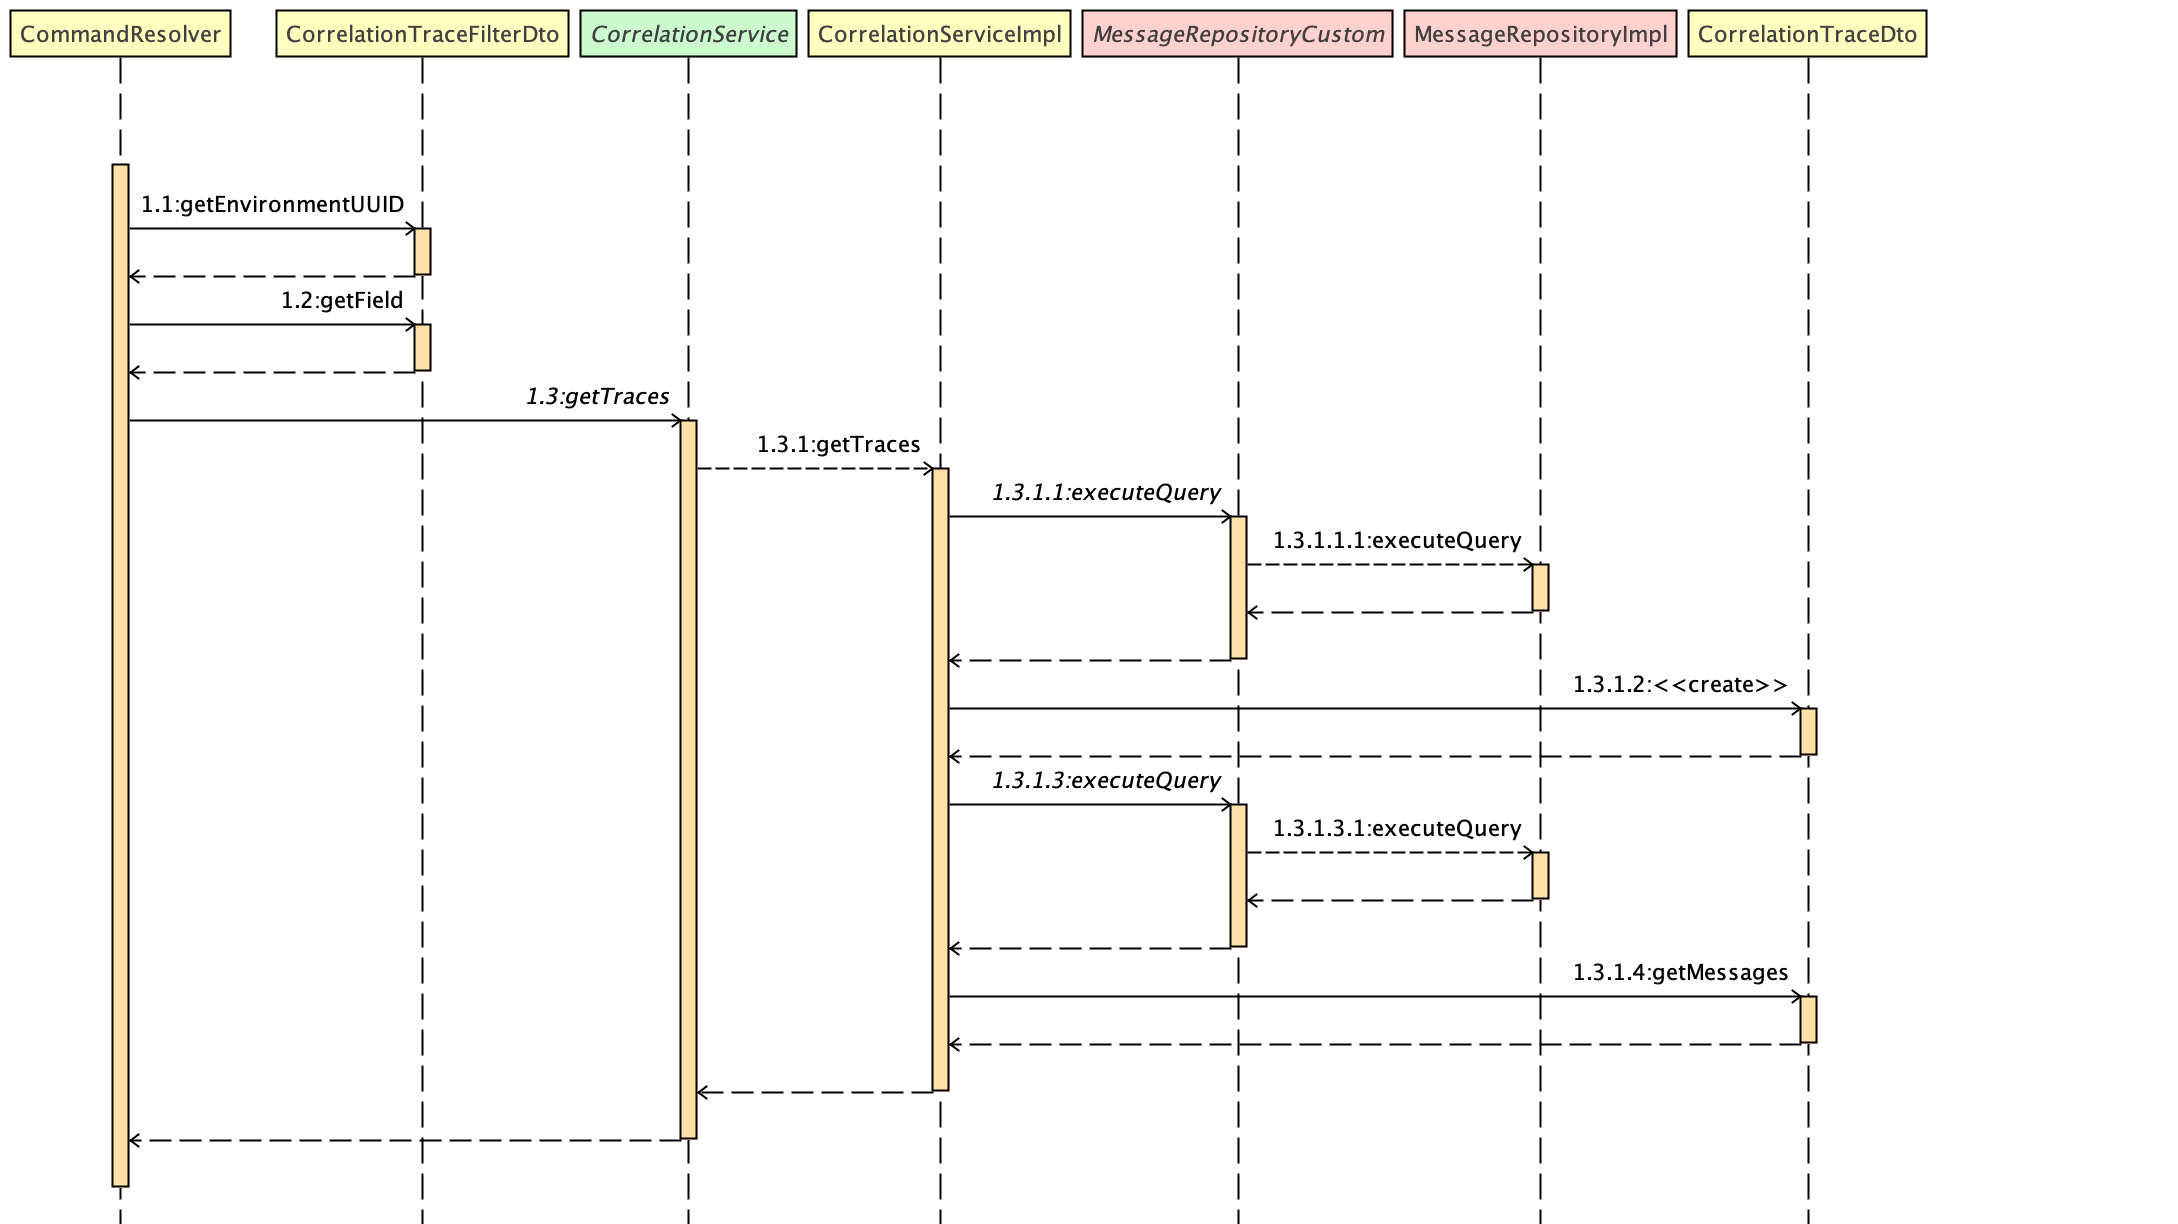
\includegraphics[width=\linewidth]{figures/impl/correlation/sequence.png}
	\caption{Sequence diagram: Requesting a correlation trace.}
	\label{correlation_svc_seq_diagram}
\end{figure}

\subsection{Correlation Algorithm}
A simple algorithm has been developed for message correlation. Correlation based on payload field value is facilitated by the Postgres-based monitored message repository, which supports JSON data types. Message payloads are persisted as JSON, allowing use of JSON-based search functions in message table queries. The Correlation Service leverages this feature when performing the following correlation steps:

\begin{itemize}
	\item Initialise an empty list \textit{L} of \texttt{CorrelationTraceDto} instances.
	\item Find all unique message field values monitored during the last hour.
	\item For each unique field value:
	\begin{itemize}
		\item Instantiate a \texttt{CorrelationTraceDto} instance \textit{CT} and add to \textit{L} .
		\item Determine the temporally-ordered set of messages whose payloads contain the unique field value.
		\item Construct a \texttt{MessageDto} for each message and add to \textit{CT}.
	\end{itemize}
\end{itemize}

 \newpage
 
 \section{Discovery Service}
 
This microservice is responsible for the discovery of environment topology information as discussed in section \ref{design_topology_discovery}, satisfying functional requirement \textit{FR-3}. It depends upon the Management Service for discovery of monitored environment information, synchronising periodically in order to start and stop sequentially executing topology discovery tasks. The implementation is agnostic of messaging technologies, in accordance with non-functional requirement \textit{NFR-2}.  A \textit{DiscoveryAgent API} provides for the implementation of varied discovery strategies, satisfying non-functional requirement \textit{NFR-1}. Two Discovery Agents, which are discussed in following sections, have been implemented as part of this prototype. Discovered topology information is registered with the Management Services via a client library exported by the latter. Discovered topology information is pushed to interested client such as the Dashboard Client using Spring WebSocket support.  This microservice is implemented as a Spring Boot application.
 
 \subsection{Modules}
 The Discovery Service comprises the modules depicted in \ref{discovery_svc_modules}. Modules which implement discovery agent plug-ins have been omitted from this diagram.
 
 \begin{figure}[H]
 	\centering  
 	\includegraphics[width=\linewidth]{figures/impl/discovery/modules.png}
 	\caption{Discovery Service modules.}
 	\label{discovery_svc_modules}
 \end{figure}

\subsection{Component Interactions}

The Discovery Service is driven by a scheduled discovery task which executes at a configurable interval, by default every five seconds. The discovery task first determines the set of currently monitored environments by polling the Management Service via its client module, as described in section \ref{management_service_external_interfaces}. The component interactions are depicted in Figure \ref{discovery_sync_task_sequence}.

\begin{figure}[H]
	\centering  
	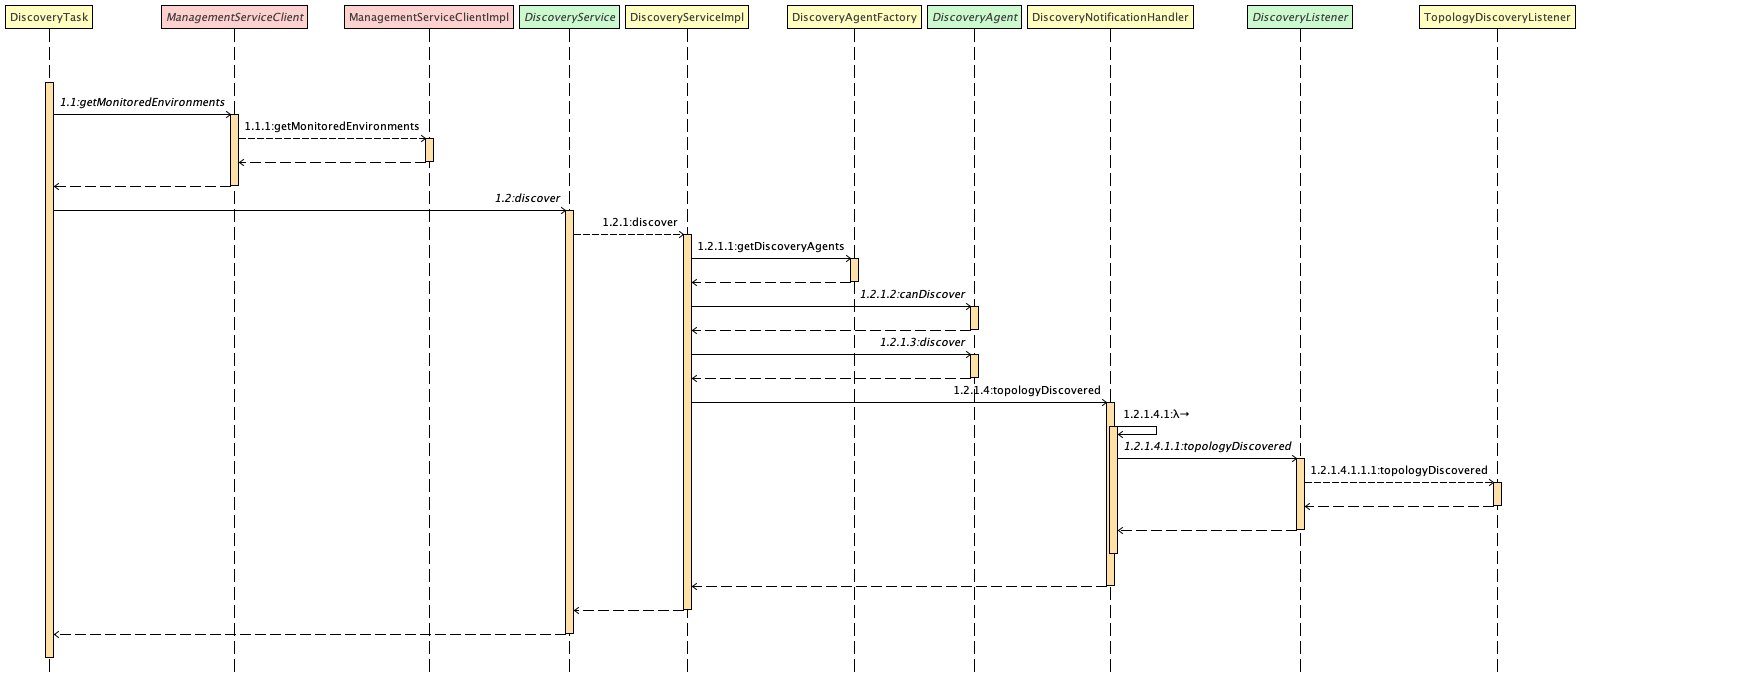
\includegraphics[width=\linewidth]{figures/impl/discovery/discovery_sequence.png}
	\caption{Discovery sequence diagram.}
	\label{discovery_sync_task_sequence}
\end{figure}

Having determined the set of currently monitored environments, the \texttt{DiscoveryTask} implementation passes these to the \texttt{DiscoveryService}, which in turns queries a \texttt{DiscoveryAgentFactory} to determine the set of available agents. For every monitored environment, the available agents are tested for applicability, and when found to be suitable candidates for environment discovery, are executed against a given environment. Discovery agent implementations are responsible for construction of \texttt{Topology} models, as described in section \ref{management_service_domain_model}. On discovery a Topology, a discovery event is dispatched to listeners registered with the \texttt{DiscoveryService}, as described in section \ref{discovery_service_notifications}.

\subsection{Discovery Agent API}
To extend the functionality of the software via addition of additional discovery strategies, the \texttt{Discovery} interface must be implemented, and the implementation class(es) made available on the runtime classpath of the Discovery Service. 

The developer of a \texttt{DiscoveryAgent} must define both Service Provider Interface (SPI) and API (Application Programming Interface) implementations. The \textit{Spring Factory} mechanism is leveraged to provide dynamic discovery and runtime auto-wiring of agent implementations \cite{SpringFactories}.

 The \texttt{DiscoveryAgent} \textit{discover()} method should construct and return an instance of \texttt{TopologyDto} to the calling application, which will in turn register the Topology with the Management Service. The Management Service will merge newly discovered Topology information with existing topology information for a given environment, preserving any existing topology structure.

This approach to topology discovery allows multiple discovery agents and strategies to construct an environment topology in a co-operative and incremental fashion if necessary.

When agent topology discovery is complete for a given scheduled execution of a \texttt{DiscoveryTask}, an asynchronous topology discovery event is dispatched to any registered listeners, as discussed in section \ref{discovery_service_notifications}.

\begin{figure}[H]
	\centering  
	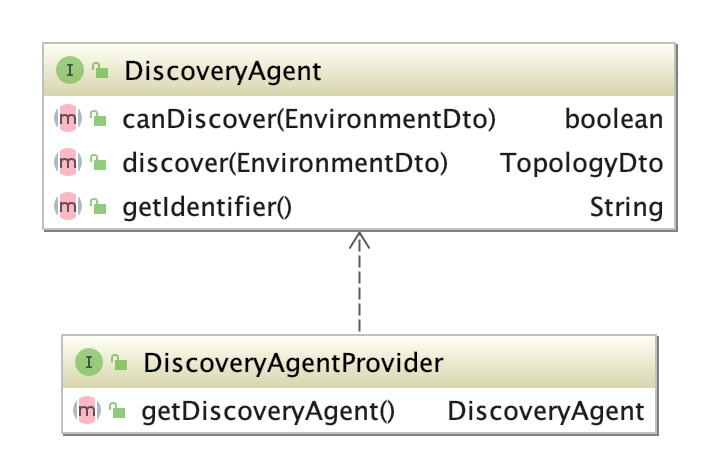
\includegraphics[scale=2.0]{figures/impl/discovery/agent_api.png}
	\caption{DiscoveryAgent SPI and API.}
	\label{discovery_agent_api}
\end{figure}

\subsection{Discovery Notifications} \label{discovery_service_notifications}
The Discovery Service implements a single external interface, closely resembling that implemented by the Aggregation Service, as described in section \ref{aggregation_service_notifications}. Clients may register for environment-specific Topology update events via a WebSocket interface.

Instances of \texttt{TopologyDto} are serialized to JSON and pushed to registered client listeners. The TopologyDto type is described by Figure \ref{topology_dto}.

\begin{figure}[H]
	\centering  
	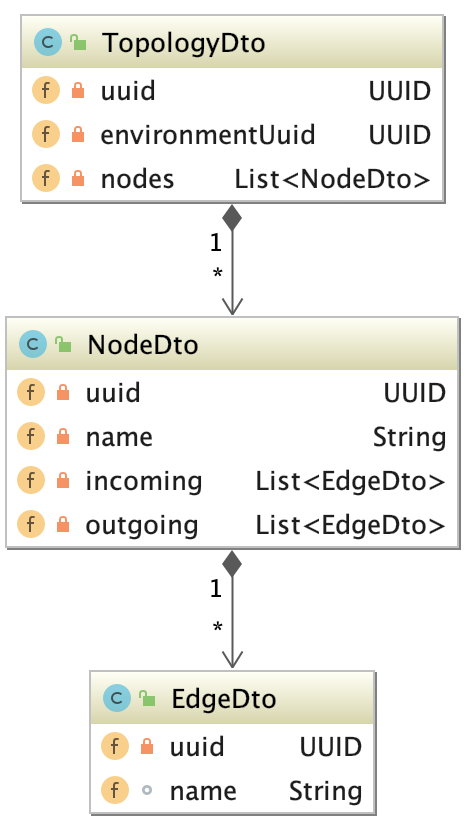
\includegraphics[scale=1.5]{figures/impl/discovery/topology_dto.png}
	\caption{Topology DTO.}
	\label{topology_dto}
\end{figure}

\subsection{Discovery Agent Implementation - Kubernetes Discovery Agent} 

The design of this agent implementation is discussed in Section \ref{design_kubernetes_discovery_agent}. The agent determines whether it can perform discovery for a given environment based on the following criteria:

\begin{itemize}
	\item The environment must define the following configuration properties:
	\begin{itemize}
	\item \texttt{discovery.agent.k8s.cert.path}: the filesystem path at which a certificate for the target Kubernetes environment can be found.
	\item \texttt{discovery.agent.k8s.namespace}:The Kubernetes namespace in which configmaps for the target environment can be discovered.
	\end{itemize}
\end{itemize}

As this agent consumes technology-agnostic metadata from Kubernetes configmaps, it is usable with various messaging technologies.

The agent is enabled by simply adding it to the classpath of the Discovery Service, as demonstrated by the following Maven POM snippet:

\begin{lstlisting}
<dependency>
  <groupId>org.cit.mcaleerj.thesis.discovery</groupId>
  <artifactId>k8s-discovery-agent</artifactId>
  <version>0.0.1-SNAPSHOT</version>
</dependency>
\end{lstlisting}

\subsection{Discovery Agent Implementation - Message Correlation}\label{discovery_service_correlation_agent} 

The design of this agent implementation is discussed in Section \ref{design_message_correlation}. The agent determines whether it can perform discovery for a given environment based on the following criteria:

\begin{itemize}
	\item The environment must define the following configuration property:
	\begin{itemize}
		\item \texttt{discovery.agent.correlation.field.name}: the message payload field used to correlate messages and construct correlation traces.
	\end{itemize}
\end{itemize}

As this agent performs correlation on technology-agnostic messages persisted by the Monitoring Service, it is usable with various messaging technologies.

The agent is enabled by simply adding it to the classpath of the Discovery Service, as demonstrated by the following Maven POM snippet:

 \vspace{5mm}
 
\begin{lstlisting}
<dependency>
<groupId>org.cit.mcaleerj.thesis.discovery</groupId>
<artifactId>message-correlation-discovery-agent</artifactId>
<version>0.0.1-SNAPSHOT</version>
</dependency>
\end{lstlisting}

 \newpage
 
 \section{User Interface Service}
 
 The User Interface service is a simple Spring Boot microservice which serves static resources required by the client dashboard application.  
 
 \section{Dashboard Client}
 
 The design of this component is discussed in section \ref{design_client_dashboard}. The Dashboard has been implemented as a Dagre-D3 based, single-page web application, served to clients by the User Interface Service. Users of the dashboard load the application by pointing a browser at the application URL, which must contain the monitored environment UUID as retrieved from the Management Service GraphQL interface. On loading, the Dashboard performs the following steps:
 
\begin{enumerate}
\item Determine the environment UUID for which the Dashboard has been opened.
\item Open a WebSocket connection to the Discovery Service, via the Gateway Service, subscribing to notifications for the given environment UUID. 
\item Open a WebSocket connection to the Aggregation Service, via the Gateway Service, subscribing to notifications for the given environment UUID. 
\item On receipt of an asynchronous event from the Discovery Service:
	\begin{enumerate}
		\item Construct a topology model by deserialising the discovery event payload.
		\item Generate a topology hash. Compare the hash value to the last rendered topology hash; ignore the discovery event if hash codes match.
		\item If topology has not already been rendered, transform the received topology object to the graph format expected by the Dagre-D3 client library, then render the graph. Furthermore, render the monitored environment name to the browser page.
	\end{enumerate}
\item On receipt of an asynchronous event from the Aggregation Service:
\begin{enumerate}
	\item Construct an EnvironmentAggregation model (see section \ref{aggregation_service_domain_model}) by deserialising the aggregation event payload.
	\item Render the aggregation window details to the browser page.
	\item For each Edge Aggregation contained in the Aggregation model, locate the corresponding graph edge, then render activity information to same.
\end{enumerate}
\end{enumerate}

The graph styling discussed in section \ref{design_topology_visualisation} has been achieved by leveraging APIs provided by the Dagre-D3 library. Results are demonstrated in Chapter 6. 

 \section{Service Registry}
 
 The Service Registry implements a simple Eureka-based discovery server. Eureka, developed by Netflix, is a REST based service which allows microservices to locate and communicate with each other without the need for hard-coding host and port details in the various co-operating service instances. The following services are configured as Eureka clients:
 
 \begin{itemize}
 	\item Management Service
 	\item Monitoring Service
 	\item Aggregation Service
 	\item Discovery Service
 	\item Correlation Service
	\item User Interface Service
	\item Gateway Service
 \end{itemize}

On startup, each service registers itself with the Service Registry, using a unique service identifier. Thereafter, lookups for the service instance endpoint information are performed via the registry. This mechanism is depicted in Figure \ref{service_registry_scheme}.
 
\begin{figure}[H]
	\centering  
	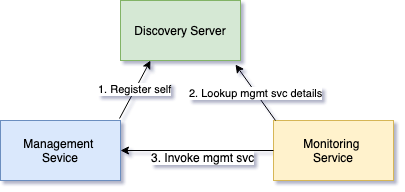
\includegraphics[scale=0.8]{figures/impl/registry/eureka_discovery.png}
	\caption{Service discovery via Service Registry.}
	\label{service_registry_scheme}
\end{figure}

\newpage

 \section{Gateway Service}
 
 The Gateway service is a Spring Boot microservice based on the Spring Cloud Gateway project. The gateway presents a single point of access for clients of the monitoring application, by routing incoming requests to downstream services, while simultaneously functioning as a proxy for asynchronous WebSocket messages. 
 
 \vspace{5mm}
 
 \begin{figure}[H]
 	\centering  
 	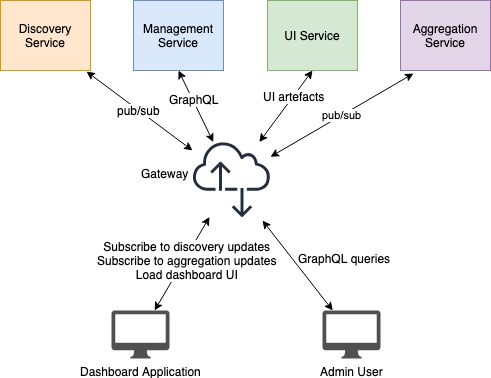
\includegraphics[scale=0.8]{figures/impl/gateway/gateway.png}
 	\caption{Gateway Service routing.}
 	\label{gatway_service}
 \end{figure}

 The following routes are implemented by the Gateway Service:
 
  \begin{itemize}
 	\item HTTP requests to load the monitoring dashboard UI are routed to the UI service.
 	\item WebSocket connections are routed to the Discovery and Aggregation services.
 	\item GraphQL requests are routed to the Management Service.
 \end{itemize}

The Gateway Service integrates with the Discovery Service, resolving route destinations via the latter service.
 
 \newpage
 
 \section{Kafka Message Producer Identification}\label{software_impl_producer_ident} 
 
 The strategy described in Section \ref{kafka_producer_header_design} has been used to develop a Spring library which enables transparent addition of message producer identifier information to Kafka messages produced by Spring applications. The library is named \textbf{spring-kafka-producer-headers}.
 
 The library comprises a single configuration class which is loaded by the Spring framework during initialisation by means of the Spring auto-configuration mechanism \cite{SpringFactories}. The configuration class returns a \texttt{BeanPostProcessor} instance to the framework; thereafter, all beans instantiated by the framework are inspected by this post-processor. The steps implemented by the post-processor are as follows:
 
 \begin{itemize}
  	\item Determine whether the passed bean is of interest - does it represent a message channel?
  	\item If so, determine whether the message channel is an output channel.
  	\item If so, add an interceptor to the channel. 
  	\item The channel interceptor will add a message header identifying the sending application to every produced message.
 \end{itemize}

To enable automatic addition of Kafka producer headers to a Spring application, a dependency on this library is simply added to the application's dependency set. No other changes are required.

For an application that uses Maven for dependency management, addition of the following dependency will enable production of Kafka headers:

\vspace{5mm}

\begin{lstlisting}[caption={Maven dependency on spring-kafka-producer-headers},captionpos=b]
<dependencies>
  <dependency>
    <groupId>org.cit.mcaleerj.thesis.spring-kafka</groupId>
    <artifactId>spring-kafka-producer-headers</artifactId>  
  </dependency>
</dependencies>
\end{lstlisting}


  

\chapter{Software Walkthrough}
\lhead{\emph{Software Walkthrough}}

This chapter contains a brief demonstrative walkthrough of the monitoring software detailed in the previous chapter, exercised against the Kubernetes / Spring Boot based test bed environment. It is provided as context for the conclusions discussed in Chapter 6.

GraphQL service interactions depicted in this chapter were performed using Insomnia GraphQL Client\cite{GraphQLI51:online}. Insomnia has been used throughout development of the prototype; one useful function of the tool is management of all operations supported by the Management Service, Correlation Service, and test bed service GraphQL interfaces. Those operations are depicted in Figure \ref{walkthough_graphql_operations}.

 \begin{figure}[H]
	\centering  
	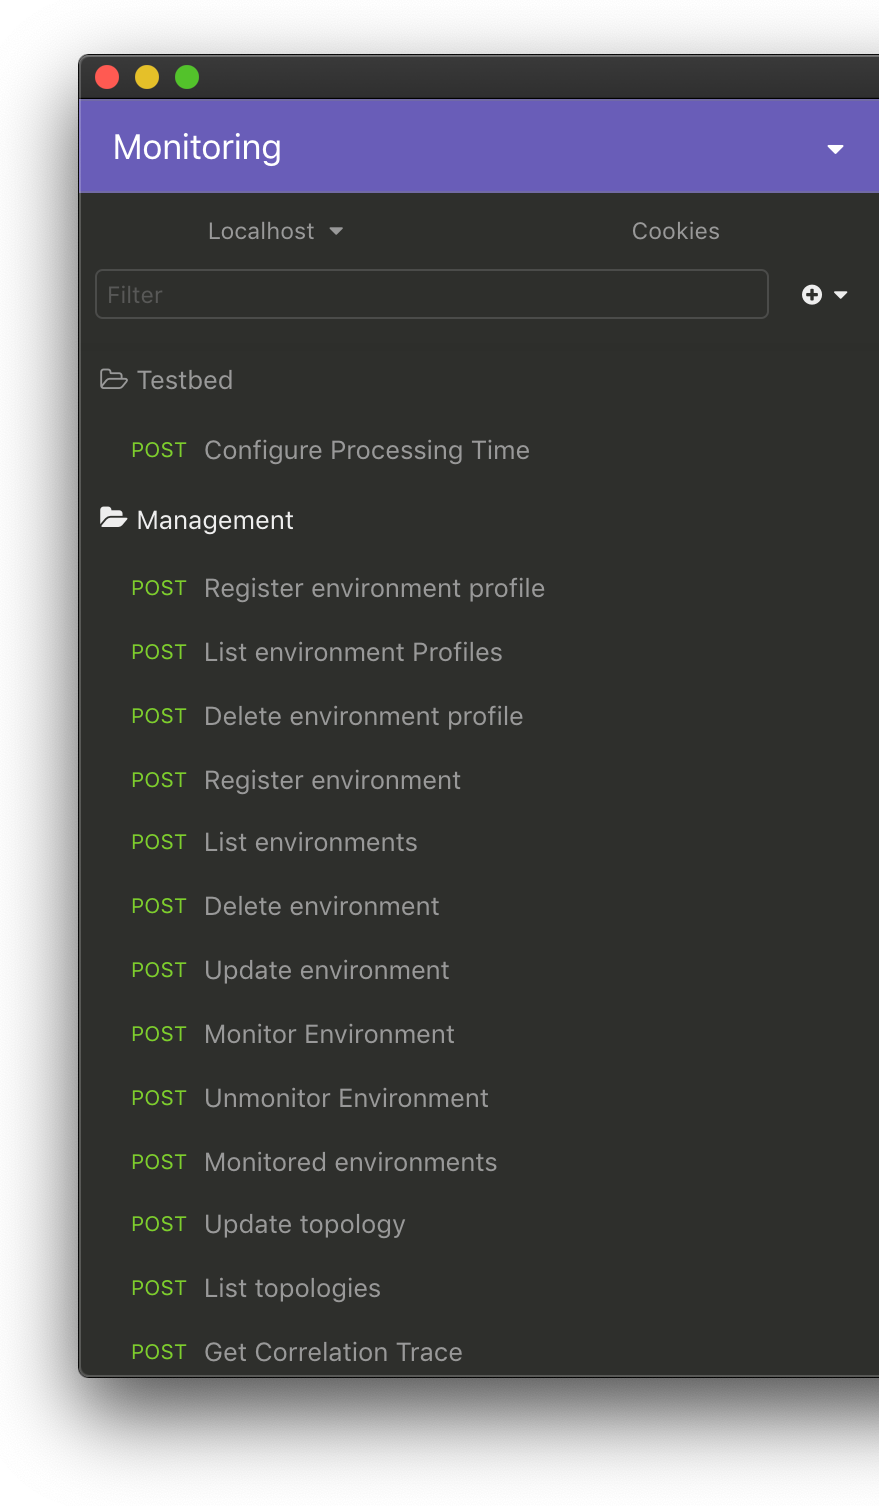
\includegraphics[scale=0.4]{figures/walkthrough/graphql_operations.png}
	\caption{GraphQL interface - All supported operations.}
	\label{walkthough_graphql_operations}
\end{figure}

\section{Kafka Environment Monitoring with the Kubernetes Discovery Agent}

\begin{enumerate}
	\item Before configuring an environment for monitoring, an environment profile must be created. In Figure \ref{walkthrough_no_profiles}, the currently defined set of environment profiles is queried at the GraphQL client. An empty list is returned by the Management Service. \linebreak

	In Figure \ref{walkthrough_create_profile}, an environment profile named \textbf{KAFKA} is created. This profile defines the monitoring task implementation applied for environments using this profile, \texttt{org.cit.mcaleerj.thesis.monitorservice.task.impl.KafkaMonitoringTask}. As the name of this Java class suggests, the task implementation monitors activity in Kafka-based applications. For an application based on RabbitMQ or ActiveMQ, an alternate classname would be specified here.

 \begin{figure}[H]
	\centering  
	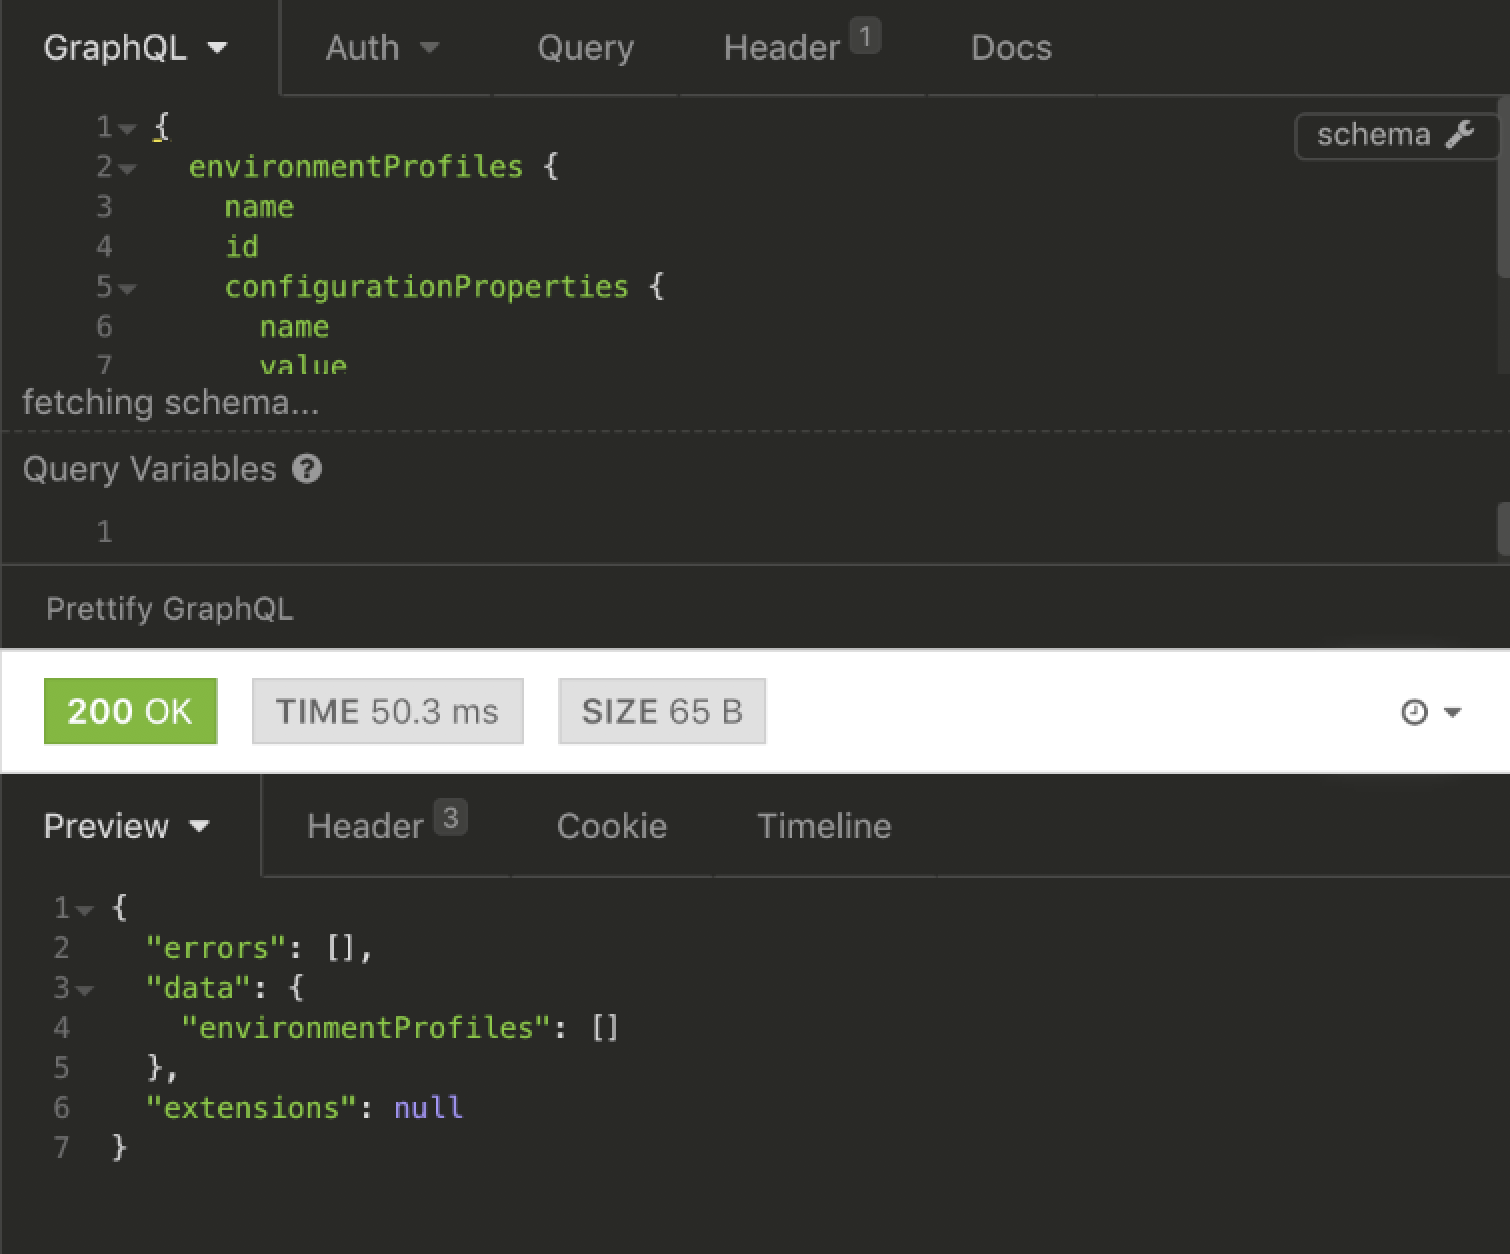
\includegraphics[scale=0.9]{figures/walkthrough/no-env-profiles.png}
	\caption{GraphQL interface - No environment profiles defined.}
	\label{walkthrough_no_profiles}
\end{figure}

 \begin{figure}[H]
	\centering  
	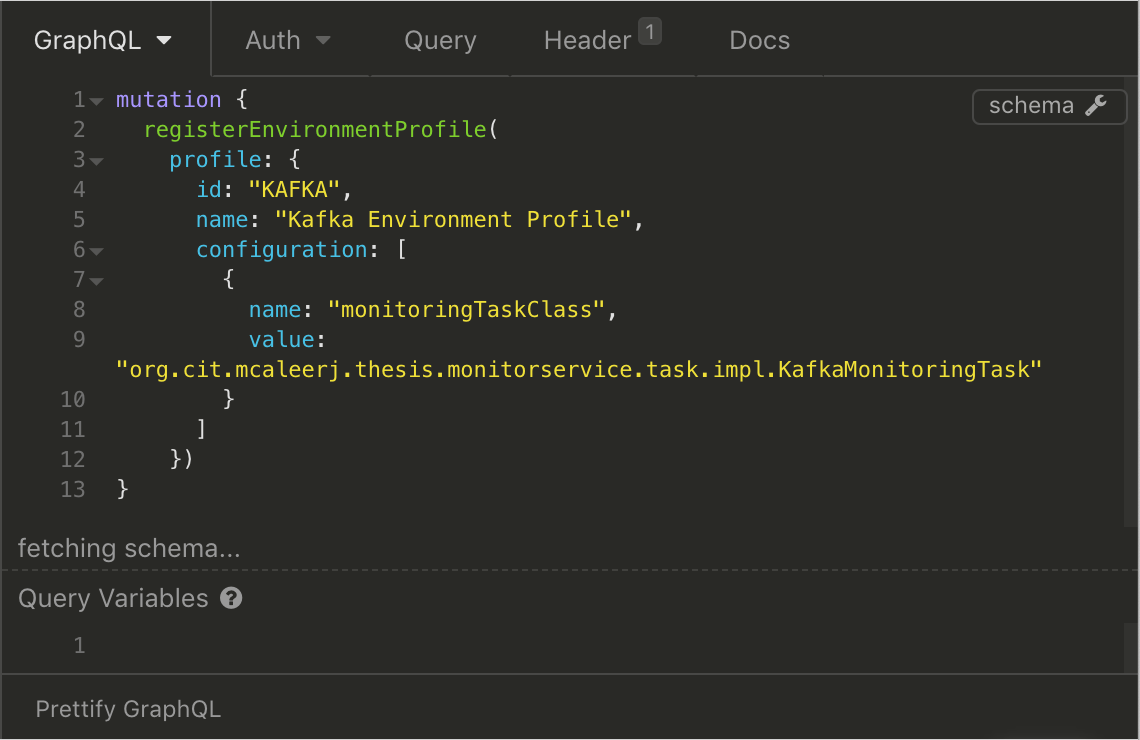
\includegraphics[scale=0.6]{figures/walkthrough/register_env_profile.png}
	\caption{GraphQL interface - KAFKA environment profile created.}
	\label{walkthrough_create_profile}
\end{figure}

	\item  In this step, an environment is defined with the following attributes:
	\begin{itemize}
		\item The environment is named \textbf{Test Environment}
		\item The environment uses the \textbf{KAFKA} profile.
		\item Configuration property \texttt{bootstrap-servers} is set to the address of the monitored application's Kafka broker: \texttt{bootstrap.kafka:9092}.
		\item Configuration property \texttt{discovery.agent.k8s.cert.path} is set to the address of a client certificate for the test bed Kubernetes cluster. This property will be read by the Kubernetes Discovery Agent.
		\item Configuration property \texttt{discovery.agent.k8s.namespace} is set to the name of the Kubernetes namespace in which the testbed pipeline will run. This property will be read by the Kubernetes Discovery Agent.
		
		 \vspace{5mm}
		 
		Figure \ref{walkthrough_env_creation} demonstrates registration of an environment using the GraphQL interface. In Figure \ref{walkthrough_env_list}, a query for the current set of registered environments returns the newly-registered environment definition. Note that a UUID is automatically generated for and assigned to newly registered environments.
		 \vspace{5mm}
  \end{itemize}
 \begin{figure}[H]
	\centering  
	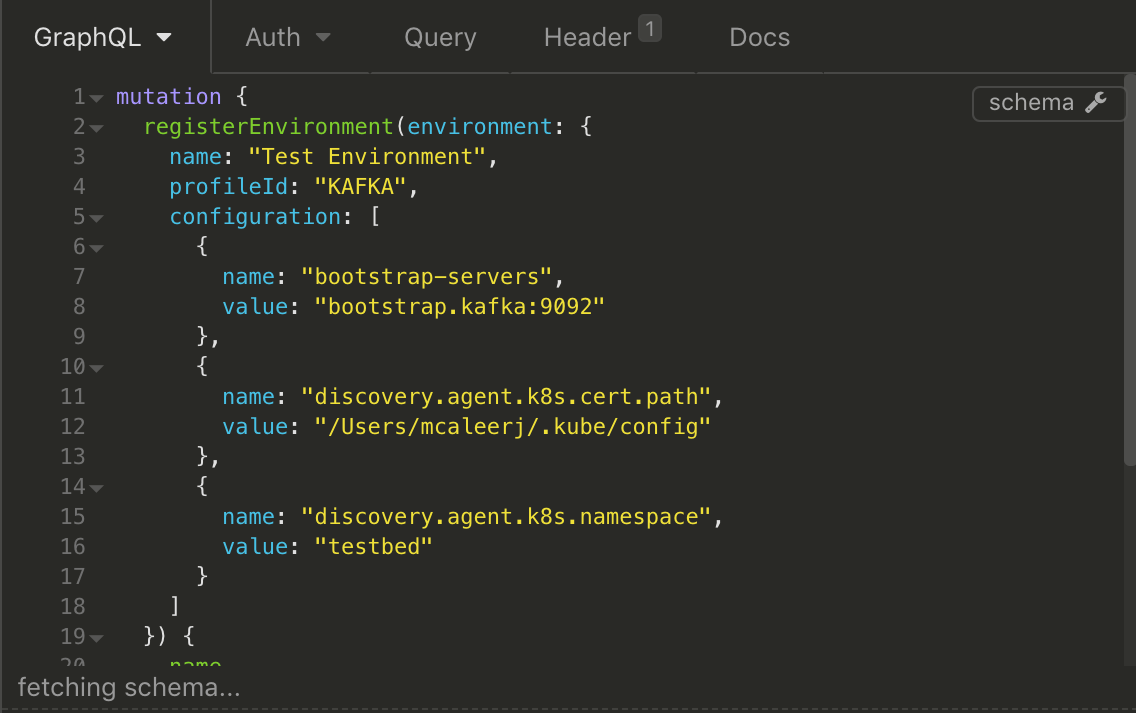
\includegraphics[scale=0.6]{figures/walkthrough/register_env.png}
	\caption{GraphQL interface - Registration of the test bed environment.}
	\label{walkthrough_env_creation}
\end{figure}

 \begin{figure}[H]
	\centering  
	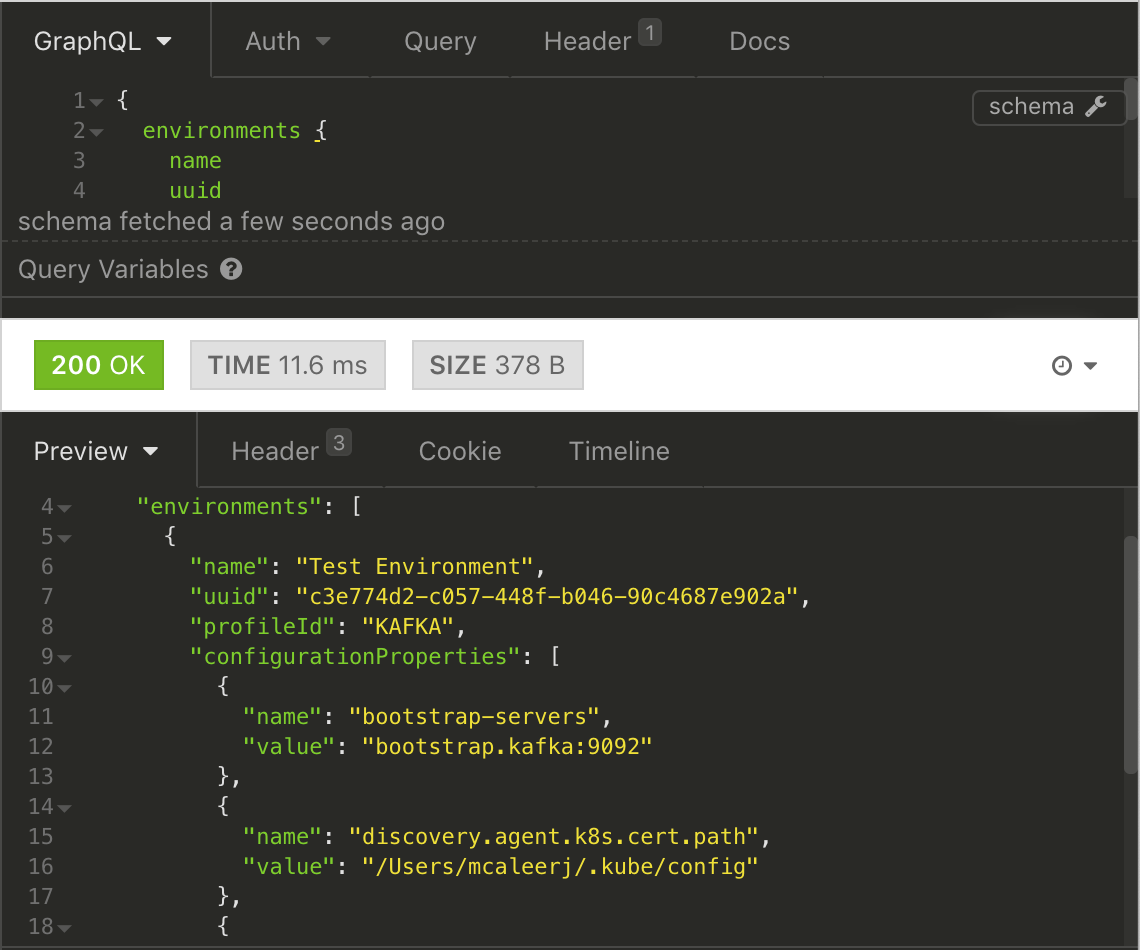
\includegraphics[scale=0.6]{figures/walkthrough/list_envs.png}
	\caption{GraphQL interface - test bed environment configuration complete.}
	\label{walkthrough_env_list}
\end{figure}

\item  In Figure \ref {walkthough_list_topologies_empty}, a query for the current set of known topologies is executed against the Management Service GraphQL endpoint. The Management Service returns an empty list. While a single environment has been registered, monitoring has not yet been enabled for the environment, and thus no discovery agents or monitoring tasks are executing against the environment as of yet.

 \begin{figure}[H]
	\centering  
	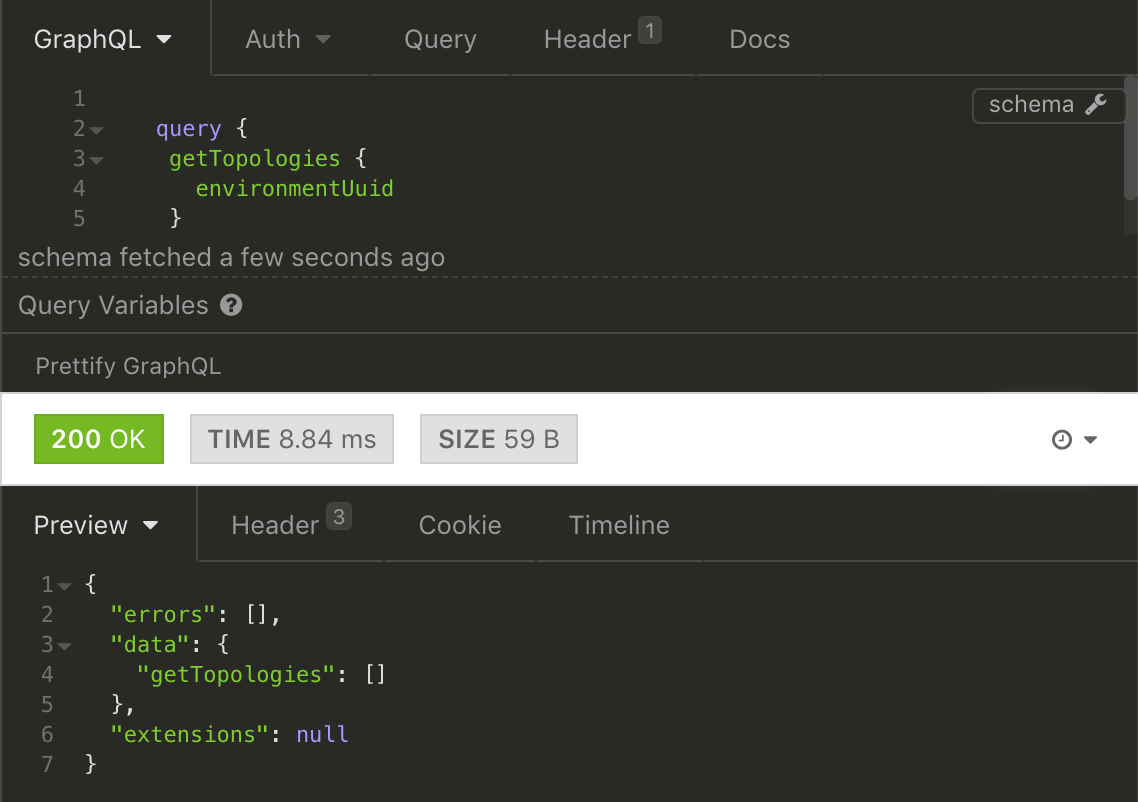
\includegraphics[scale=0.6]{figures/walkthrough/no_topologies.png}
	\caption{GraphQL interface -  No topologies defined.}
	\label{walkthough_list_topologies_empty}
\end{figure}

\item  Using the generated UUID for the environment registered in previous steps, environment monitoring is enabled in Figure \ref{walkthough_enabled_monitoring}.

 \begin{figure}[H]
	\centering  
	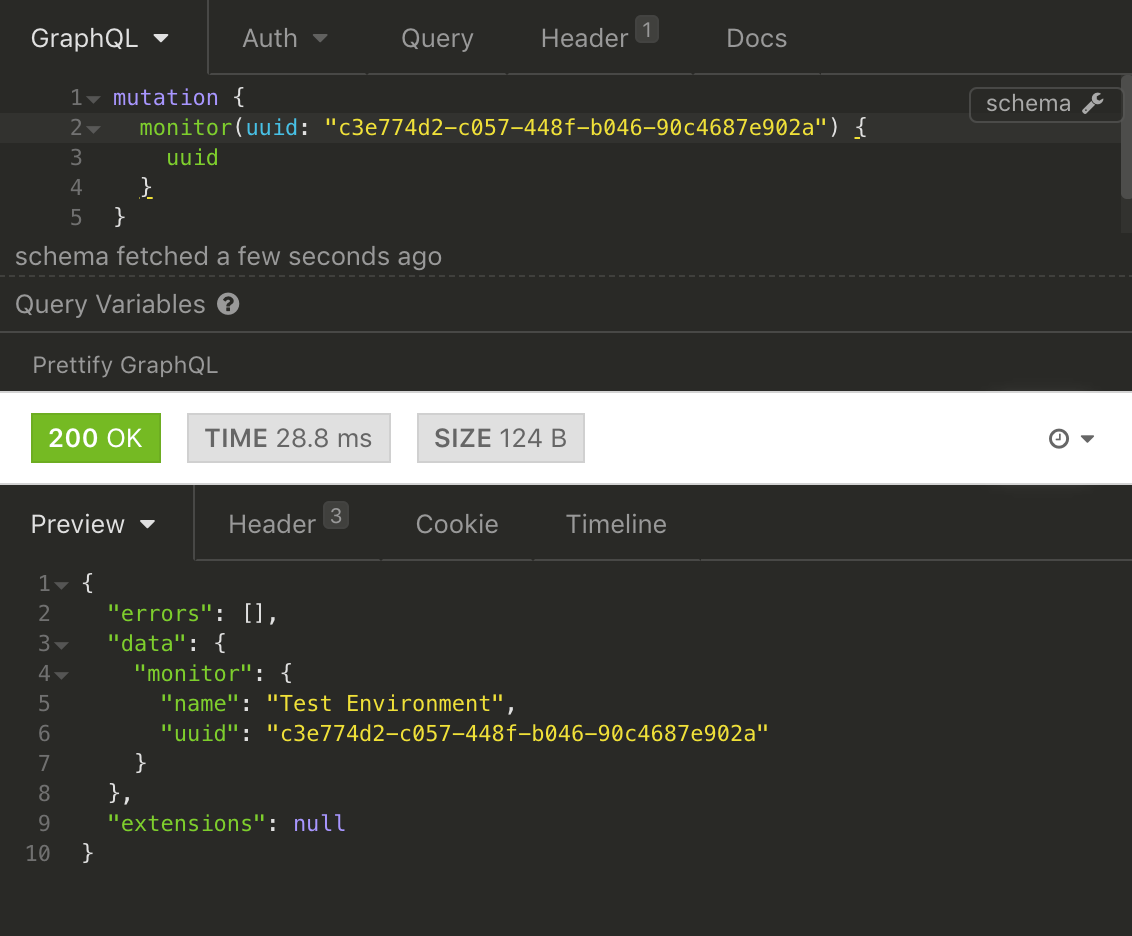
\includegraphics[scale=0.6]{figures/walkthrough/enable_monitoring.png}
	\caption{GraphQL interface -  Enabling monitoring for the test bed environment.}
	\label{walkthough_enabled_monitoring}
\end{figure}

\item The Dashboard Client is opened for the monitored environment. No topology is displayed, as the test bed application has not yet been deployed. The empty topology rendition is portrayed in Figure \ref{walkthough_empty_topology}.

 \begin{figure}[H]
	\centering  
	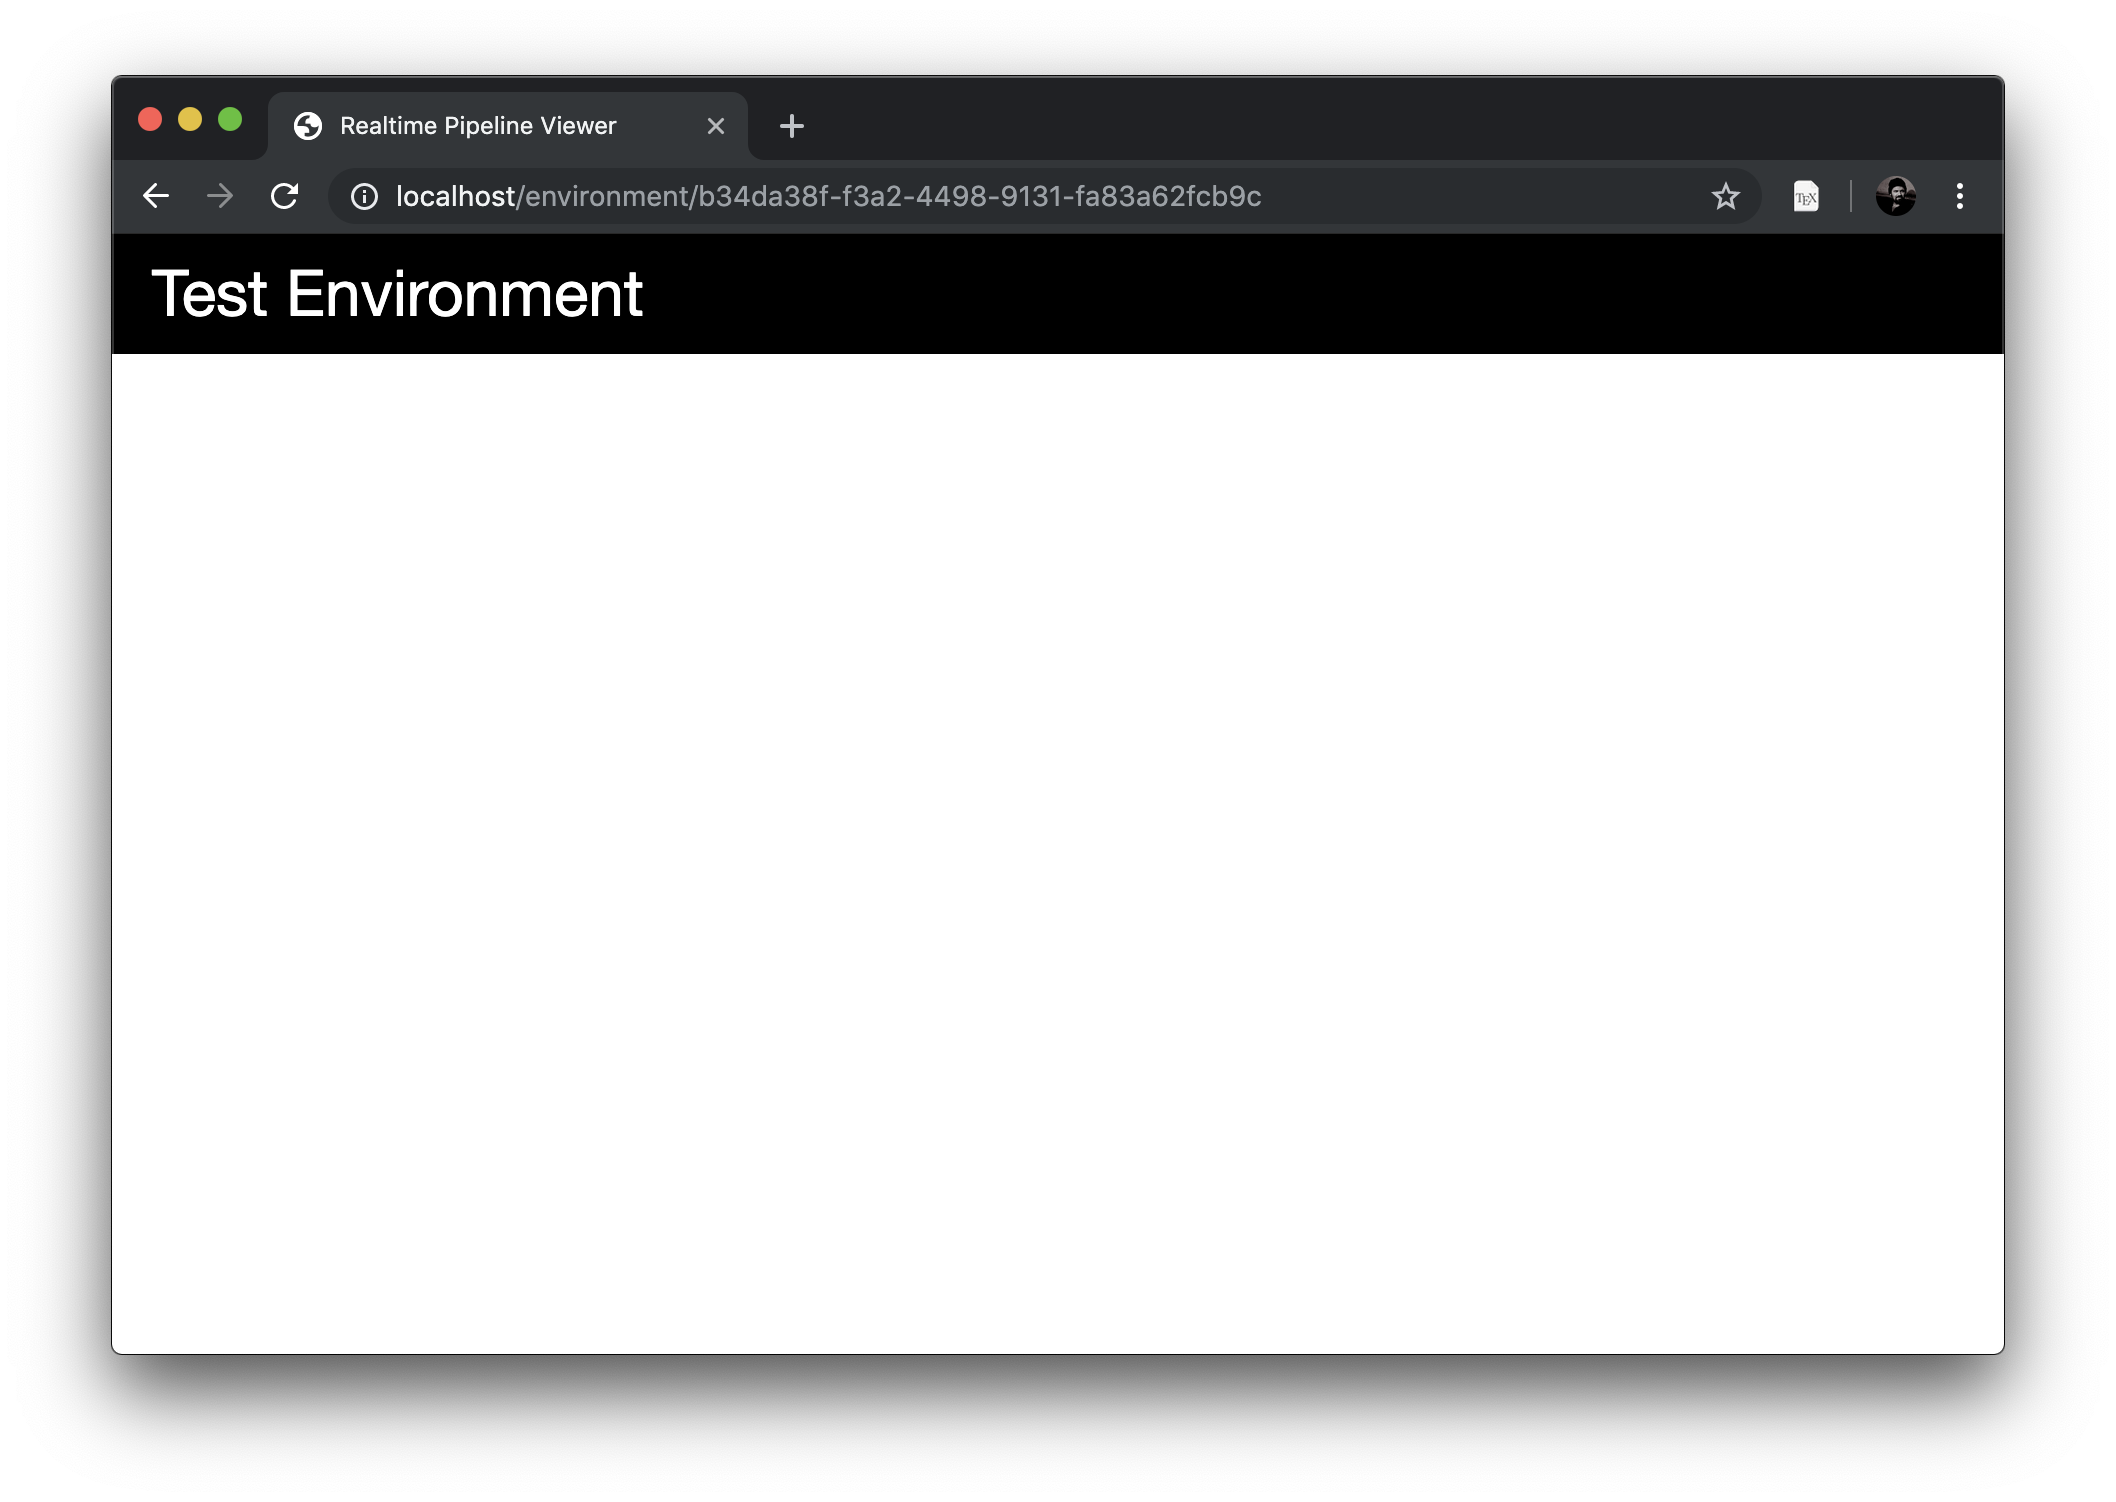
\includegraphics[scale=0.3]{figures/walkthrough/env-zero-nodes.png}
	\caption{Dashboard Client - test bed environment contains an empty topology.}
	\label{walkthough_empty_topology}
\end{figure}

\item Following the steps described in Appendix A, the first of the test bed environment microservices is deployed. The Dashboard Client automatically updates to reflect this change, as depicted in Figure \ref{walkthough_one_node_topology}. The green node indicates an external message source, while the light blue node represents a microservice; the red node meanwhile represents a message sink.

\begin{figure}[H]
	\centering  
	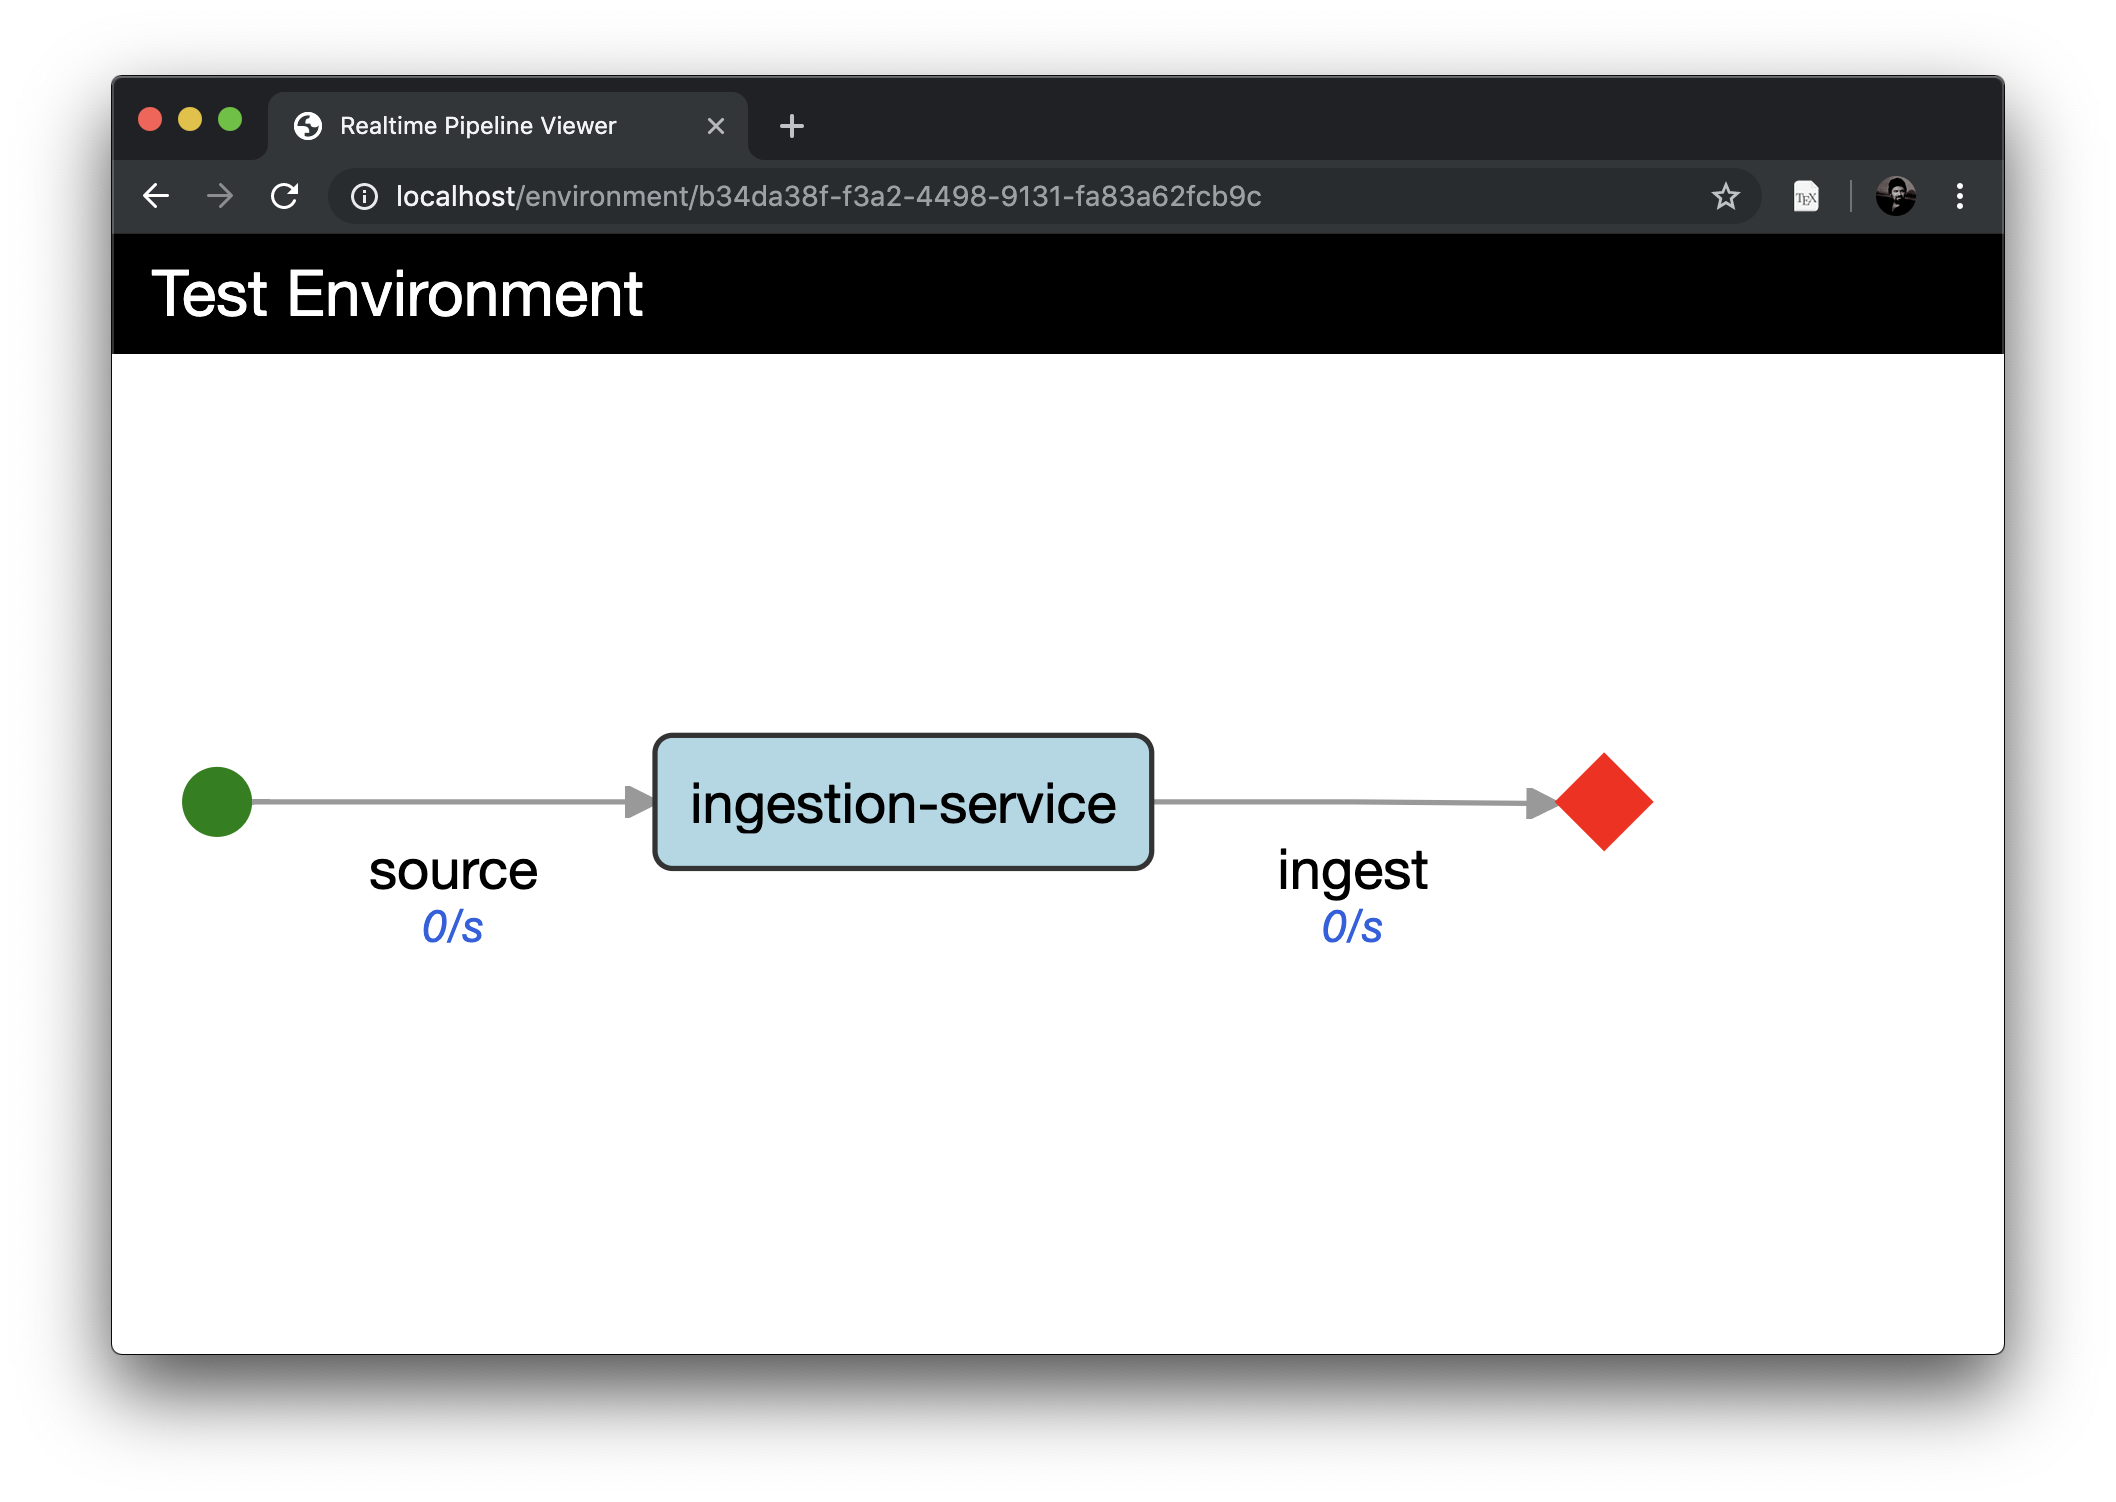
\includegraphics[scale=0.3]{figures/walkthrough/env-one-node.png}
	\caption{Dashboard Client - test bed environment comprising a single microservice.}
	\label{walkthough_one_node_topology}
\end{figure}

\item A second microservice is now deployed; the Dashboard Client again reflects this change automatically, as depicted in Figure \ref{walkthough_two_node_topology}. The ingest edge is no longer rendered as a message sink, as the newly-deployed validation-service is known to consume from same. Two new sink edge are added, namely the \texttt{validated} and \texttt{deadletter} edges.

\begin{figure}[H]
	\centering  
	\includegraphics[scale=0.3]{figures/walkthrough/env-two-nodes.png}
	\caption{Dashboard Client - test bed environment comprising two microservices.}
	\label{walkthough_two_node_topology}
\end{figure}

\item The third and final microservice is now deployed; the Dashboard Client again reflects this change automatically, as depicted in Figure \ref{walkthough_three_node_topology}. The validated edge is no longer rendered as a message sink, as the newly-deployed sink-service is known to consume from same. One new sink edge is added, namely the \texttt{processed} edge.

\begin{figure}[H]
	\centering  
	\includegraphics[scale=0.3]{figures/walkthrough/env-three-nodes.png}
	\caption{Dashboard Client - test bed environment comprising three microservices.}
	\label{walkthough_three_node_topology}
\end{figure}

\item Note that edge labels indicate environment activity of zero messages per seconds on all edges in the topology. A message generator is now executed, pushing approximately thirty messages per second to the monitored environment. Topology activity is accurately reflected in real-time by the Dashboard Client, as depicted in Figure \ref{walkthough_thirty_messages_sec}.

\begin{figure}[H]
	\centering  
	\includegraphics[scale=0.3]{figures/walkthrough/topology_30_sec.png}
	\caption{Dashboard Client - test bed topology processing thirty messages per second.}
	\label{walkthough_thirty_messages_sec}
\end{figure}\

\item The number of messages pushed into the monitored environment is now dropped to approximately ten messages per second. The change in environment throughput is reflected immediately at the Dashboard Client, as depicted in Figure \ref{walkthough_ten_messages_sec}.

\begin{figure}[H]
	\centering  
	\includegraphics[scale=0.3]{figures/walkthrough/topology_10_sec.png}
	\caption{Dashboard Client - test bed topology processing ten messages per second.}
	\label{walkthough_ten_messages_sec}
\end{figure}

\item The number of messages per second pushed to the environment is restored to thirty per second. An artificial message processing delay is introduced at the validation service, by means of a GraphQL interface provided by same.  The processing bottleneck introduced by this configuration change is clearly reflected by the drop off in throughput on edge \textit{validated}, as demonstrated by Figure \ref{walkthough_bottleneck}.

\begin{figure}[H]
	\centering  
	\includegraphics[scale=0.3]{figures/walkthrough/validation_bottleneck.png}
	\caption{Dashboard Client - artificial bottleneck at the validation service.}
	\label{walkthough_bottleneck}
\end{figure}

\end{enumerate}

\section{Environment Monitoring with the Message Correlation Discovery Agent}

\begin{enumerate}
	
	\item A new environment is registered with the monitoring application. For this environment, properties required by the Kubernetes Discovery Agent are not configured. Instead, the Message Correlation Discovery agent is configured by setting environment configuration property \texttt{discovery.agent.correlation.field.name} to \texttt{uuid}. 
	
	Test message payloads sent to the monitored environment each contain a unique UUID field named \texttt{uuid}. The Discovery Agent will leverage this fact, requesting correlation traces based on the configured field from the Correlation Service in order to construct a topology instance. The GraphQL mutation used to configure the newly created environment is depicted in Figure  \ref{reg_env_correlation}.
	
	\vspace{5mm}
		 
\begin{figure}[H]
	\centering  
	\includegraphics[scale=0.7]{figures/walkthrough/correlation_env.png}
	\caption{Dashboard Client - configuring an environment for correlation-based discovery.}
	\label{reg_env_correlation}
\end{figure}

	\item In contrast to the sequence of events described in the previous section on Kubernetes-based discovery, no topology is rendered until messages begin to flow through the environment. Once a number of messages have traversed the environment, the Dashboard Client renders the topology as depicted in Figure  \ref{activity_env_correlation}.

\begin{figure}[H]
	\centering  
	\includegraphics[scale=0.4]{figures/walkthrough/correlation_env_activity.png}
	\caption{Dashboard Client - message activity in an environment discovered by message correlation.}
	\label{activity_env_correlation}
\end{figure}


\end{enumerate} 

\chapter{Conclusions and  Further Development}
\lhead{\emph{Conclusions and  Further Development}}

The research conducted, and software implemented, during the course of this dissertation demonstrate that real-time monitoring of message-driven pipelines is an achievable goal for developers, testers and maintainers of such environments. By rendering pipeline state in a readily consumable and accessible fashion, answers to questions such as the following are readily available:


\begin{itemize}
	\item What microservices currently comprise my pipeline application?
		    \begin{itemize}
		    	\item Scan the pipeline topology graph to yield the set of microservices.
		    \end{itemize}
	\item On what topics are my pipeline microservices communicating?
	 	\begin{itemize}
			\item Scan the pipeline topology graph to yield the set of edge labels.
		\end{itemize}
	\item What activity, if any, is occurring on my pipeline at this moment?
	 	\begin{itemize}
			\item Scan the pipeline topology graph for edge activity information.
		\end{itemize}
	\item Are any of my pipeline microservices currently down?
		\begin{itemize}
			\item Scan the pipeline topology graph for nodes with activity on incoming edges but no corresponding outgoing activity.
		\end{itemize}
	\item What bottlenecks exist in my pipeline at present?
			\begin{itemize}
				\item Scan the pipeline topology graph for nodes with activity on incoming edges but comparatively little outgoing activity.
			\end{itemize}
    \item Are messages successfully traversing the entire pipeline?
    		\begin{itemize}
    			\item Scan the pipeline topology graph for activity on edges connected to sink nodes.
    		\end{itemize}
    \item What are the source message topics for my pipeline?
    		\begin{itemize}
				\item Scan the pipeline topology graph for edges connected to source nodes.
			\end{itemize}
    \item What are the sink message topics for my pipeline?
    	\begin{itemize}
    		\item Scan the pipeline topology graph for edges connected to sink nodes.
    	\end{itemize}
\end{itemize}

The implemented monitoring prototype establishes that the rendition of application state can dynamically reflect pipeline topology evolution over time. Furthermore, the core implementation successfully abstracts specific messaging technologies, and has been shown to function as designed as a monitoring tool for Kafka-based pipelines. Overall, all functional and non-functional requirements set out in section \ref{project_requirements} have been implemented successfully.

The implemented solutions to the key challenges presented by this research and implementation - edge correlation, topology discovery, and topology visualisation will be evaluated on various criteria including reliability, applicability, scalability, and level of invasiveness. 

Edge correlation has been implemented by developing a Spring library which, once added to the runtime class path of a Spring application, will automatically add message sender information to all produced Kafka messages. This solution is relatively non-invasive, requiring an update to the application class path only; it is also an absolute prerequisite for message-to-edge correlation. Once added to an application, the solution should be fully reliable and scalable. From an applicability perspective, this solution is very specific to Spring applications which use Kafka as a messaging technology. For applications which are not implemented with Java and Spring, alternative solutions must be developed. 

Various approaches to topology discovery have been implemented. Manual topography configuration (section \ref{design_topology_discovery}) is reliable and applicable to various messaging technology types, but may require significant manual work as well as ongoing maintenance as pipeline state evolves. Furthermore, expertise in use of the monitoring application prototype is required in order to perform topology management. The Kubernetes Discovery Agent in contrast requires less expertise and less maintenance, providing parties responsible for application deployment annotate configmaps with the prescribed metadata; it too is agnostic of message technology has as such has broad applicability; with the proviso that the pipeline application is deployed to a Kubernetes cluster. This implementation serves to demonstrate that in general, pipeline metadata may be derived from the monitored pipeline's runtime environment, as is done by the Kiali monitoring solution. Finally, as has been shown in section \ref{design_message_correlation}, discovery based on message correlation, while non-invasive, is applicable only to pipeline applications with appropriate topology structures, and requires accurate message timestamp information which may not always be available in a distributed environment.

While pipeline visualisation has been demonstrated successfully, the prototype implementation will exhibit shortcomings when applied to pipelines comprising large numbers of nodes. During early prototyping it was found that screen real estate became an issue when rendering manually constructed topologies comprising in excess of approximately twenty nodes to a 1080p display. Existing monitoring solutions such as Kiali and StreamSets would appear to suffer a similar shortcoming.

Ultimately, it has been demonstrated that while real-time monitoring is practical for Kafka-based pipeline applications, some invasive change to the pipeline software, or tight integration with an instrumented deployment environment is an unavoidable prerequisite. It has been demonstrated that a technology-agnostic solution implementation is achievable. By comparison to for instance Kiali, which features comparable topology discovery and activity monitoring functionality), this solution places no strict dependency requirements, such as Istio integration, on pipeline implementations.

Several aspects of the research performed and software implemented during the course of this dissertation may merit further investigation. Foremost amongst these are opportunities to enhance the Aggregation Service with the goal of providing additional useful information to users. By exploiting historical aggregation information, functionality allowing users to inspect monitored environment during the past would be achievable. Furthermore, additional useful metrics might be calculated by the aggregation logic, such a minimum, maximum and average throughput per edge over time. Visualisation enhancements could include styling of edge graphics to communicate more readily which monitored microservices are responsible for bottlenecking. 

The author has considered the implementation of additional services such as a \textit{Decorator Service}, which would define a plug-in interface allowing for custom decoration of graph nodes at the Dashboard Client. This would allow the client application to render information such a service liveness, links to service logs and JMX statistics. While exploration of such functionality was not scoped for this dissertation, such enhancements would add considerable value to the solution, while also introducing the possibility of interactive dashboards.

The basic Correlation Service prototype might be enhanced to support visual correlation traces based on more flexible correlation criteria. For example, a Dashboard Client user might requests a correlation trace for message containing the payload property / value pair \textit{"foo": "bar"}. The correlation engine, enhanced to support configurable and extensible correlation rules, would provide trace information to the Dashboard which would in turn visually render the trace for user analysis.

Ideally, monitoring and topology discovery plugins could be developed in the course of any future work, allowing for monitoring of disparate pipeline applications based on various messaging technologies. 

Finally, tractability limitations around the rendering of pipelines containing large numbers of services might be explored in any future development of this research area. 

%% ----------------------------------------------------------------
\label{Bibliography}
\lhead{\emph{Bibliography}}
\bibliographystyle{IEEEtranN}  % Use the "IEEE Transaction" BibTeX style for formatting the Bibliography
\bibliography{Bibliography}  % The references (bibliography) information are stored in the file named "Bibliography.bib"
\lhead{\emph{Bibliography}}  % Change the left side page header to "Bibliography"

%% ----------------------------------------------------------------
% Now begin the Appendices, including them as separate files

\addtocontents{toc}{\vspace{2em}} % Add a gap in the Contents, for aesthetics

\begin{appendices}
	
\chapter{Test Environment Setup and Verification}
\lhead{\emph{Appendix A - Test Environment Setup and Verification}}  

A dedicated environment has been developed for purposes of development testing. The environment comprises a Kubernetes cluster running a microservices-based pipeline application, supported by Kafka and Zookeeper instances. The pipeline application and messaging infrastructure run in dedicated Kubernetes namespaces  \textit{testbed} and  \textit{kafka}, respectively. Environment prerequisites, configuration and validation are detailed in the following sections.

\section{Prerequisites}
\begin{enumerate}
	
 \item Install a recent Java Development Kit on your host environment. 
	
 \item Install a recent Python runtime on your host environment. Additionally, install Kafka tools for Python:
 
 \begin{lstlisting}[language=bash]
 $ pip install kafka-python
 \end{lstlisting}

\item Install a recent version of Maven by following the instructions provided at:

https://maven.apache.org/users/index.html. 
	
 \item Install Docker by following the instructions appropriate for your OS. Documentation is available at https://docs.docker.com/install.
	
	
 \item Install Minikube by following the steps detailed at \linebreak https://kubernetes.io/docs/tasks/tools/install-minikube.

\end{enumerate}

\section{Configuration}

\begin{enumerate}
	
 \item The various required configuration scripts are bundled with the project implementation sources at https://github.com/schmigware/monitoring-app. Clone this repository to your local environment by issuing following command: 

\begin{lstlisting}[language=bash]
$ git clone https://github.com/schmigware/monitoring-app
\end{lstlisting}

 \item Start the Minikube Kubernetes cluster by executing the script \texttt{config/startcluster.sh}

\begin{lstlisting}[language=bash]
$ cd kubernetes
$ ./startcluster.sh
\end{lstlisting}

Minikube will echo startup status to the console.

\begin{figure}[H]
	\centering  
	\includegraphics[width=\linewidth]{figures/appendixA/minikube-startup.png}
	\caption{Minikube cluster startup.}
\end{figure}


 \item The Zookeeper/Kafka configuration files bundled with the project are customised versions of those provided by open source project https://github.com/Yolean/kubernetes-kafka. A single Kafka broker is defined; importantly, auto-creation of Kafka topics is enabled for the cluster. To create the various required namespaces and services, execute the script \texttt{config/configurecluster.sh}. Cluster configuration may take several minutes while persistent volumes are initialised.

\begin{lstlisting}[language=bash]
$ ./configurecluster.sh
\end{lstlisting}


 \item Verify that the \texttt{kafka} namespace has been created correctly by issuing the following kubctl command:
 
 \begin{lstlisting}[language=bash]
 $ kubectl get namespaces
 \end{lstlisting}

The output should list the expected namespace.

\begin{figure}[H]
	\centering  
	\includegraphics[width=\linewidth]{figures/appendixA/namespaces.png}
	\caption{Verification of kafka namespace creation.}
\end{figure}

 \item Verify that the \texttt{kafka} namespace contains running Kafka and Zookeeper pods by issuing the following kubctl command, which lists all pods for the namespace in question:

\begin{lstlisting}[language=bash]
$ kubectl get pods -n kafka
\end{lstlisting}

The output should contain Kafka and Zookeeper pods.

\begin{figure}[H]
	\centering  
	\includegraphics[width=\linewidth]{figures/appendixA/kafka-pods.png}
	\caption{Verification of Zookeeper/Kafka pod creation.}
\end{figure}


 \item Cluster state can be further verified via the Minikube Dashboard. To start the dashboard, issue the following command:
 
 \begin{lstlisting}[language=bash]
 $ minikube dashboard
 \end{lstlisting}
 
 When the dashboard opens, navigate to the \texttt{kafka} namespace. Workload status images should be displayed in green. 
 
 \begin{figure}[H]
 	\centering  
 	\includegraphics[width=\linewidth]{figures/appendixA/dashboard-kafka.png}
 	\caption{Minikube Dashboard status for the \texttt{kafka} namespace.}
 \end{figure}

 \item While cluster endpoints are typically exposed using Kubernetes Services, this approach presents some difficulties when exposing a Kafka bootstrap server, as the server presents clients with cluster-internal broker IP addresses which will not be resolvable by cluster-external clients. This issue can be circumvented by configuring a VPN into the cluster, using a solution such as \textit{Telepresence}. Install Telepresence by following the instructions at https://www.telepresence.io/.
 
 \item Start a VPN from your host OS to the Kubernetes cluster by executing the following command. As a prerequisite step, determine the cluster-inter Kafka broker IP address via the Minikube dashboard,
 
 \begin{lstlisting}[language=bash]
$ telepresence --run-shell --also-proxy broker.kafka --also-proxy zookeeper.kafka  
--also-proxy <kafka broker internal ip address>
\end{lstlisting}

 \begin{figure}[H]
	\centering  
	\includegraphics[width=\linewidth]{figures/appendixA/start-telepresence.png}
	\caption{Telepresence startup.}
\end{figure}

 \item To test cluster connectivity, start a Kafka console consumer, pointing it to the Kafka broker running within the Kubernetes cluster. As topic auto-creation is enabled, configure the tool to listen on an arbitrary topic such as \texttt{test-topic}:
 
  \begin{lstlisting}[language=bash]
 $ kafka-console-consumer --bootstrap-server bootstrap.kafka:9092 --topic test-topic
 \end{lstlisting}

 \item Next, send a message to the topic chosen in the previous step:
 
  \begin{lstlisting}[language=bash]
 $ kafka-console-producer --broker-list broker.kafka:9092 --topic test-topic
 \end{lstlisting}

 \begin{figure}[H]
	\centering  
	\includegraphics[width=\linewidth]{figures/appendixA/send-test-message.png}
	\caption{Sending a test message to topic \textit{test-topic}.}
\end{figure}


 \item The kafka consumer should now echo the text message. If so, the Zookeer/Kafka environment and Telepresence VPN are configured correctly.

\begin{figure}[H]
	\centering  
	\includegraphics[width=\linewidth]{figures/appendixA/consume-test-message.png}
	\caption{Receiving a test message on topic \textit{test-topic}.}
\end{figure}


 \item Next, configure the test pipeline microservices. The various applications are bundled with the project implementation sources at https://github.com/schmigware/monitoring-app. Change directory to \texttt{/software/test-environment}. Execute the following commands to configure security roles and a new namespace,  \textbf{testbed}.

  \begin{lstlisting}[language=bash]
$ kubectl apply -f k8s/testbed-namespace.yml
$ kubectl apply -f k8s/serviceaccount.yml -n testbed
\end{lstlisting}

 \item Verify that the \texttt{testbed} namespace has been created correctly by issuing the following kubctl command:

\begin{lstlisting}[language=bash]
$ kubectl get namespaces
\end{lstlisting}

The output should list the expected namespace.

\begin{figure}[H]
	\centering  
	\includegraphics[width=\linewidth]{figures/appendixA/testbed-namespace.png}
	\caption{Verification of kafka namespace creation.}
\end{figure}

 \item Build the various microservice projects by issuing the following commands from the directory  \texttt{/software/test-environment}. The first shell command forces the Maven Docker build task to build microservice images using Minikube's Docker registry.
 
  \begin{lstlisting}[language=bash]
 $ eval $(minikube docker-env)  
 $ maven clean install
 \end{lstlisting}


\item Create Kubernetes deployments for the \textit{ingestion}, \textit{validation} and \textit{sink} test bed services by executing the following commands in order. 

\begin{lstlisting}[language=bash]

$ kubectl apply -f ingestion-service/application/k8s/configmap.yml
$ kubectl apply -f ingestion-service/application/k8s/deployment.yml

$ kubectl apply -f validation-service/application/k8s/configmap.yml
$ kubectl apply -f validation-service/application/k8s/deployment.yml

$ kubectl apply -f sink-service/application/k8s/configmap.yml
$ kubectl apply -f sink-service/application/k8s/deployment.yml
\end{lstlisting}

 \item Verify that the \texttt{testbed} namespace contains running microservice applications by issuing the following kubctl command, which lists all pods for the namespace in question:

\begin{lstlisting}[language=bash]
$ kubectl get pods -n testbed
\end{lstlisting}

The output should list three running pods:

\begin{figure}[H]
	\centering  
	\includegraphics[width=\linewidth]{figures/appendixA/testbed-pods.png}
	\caption{Verification of test bed pod creation.}
\end{figure}

 \item Furthermore, the test bed pipeline microservices should be reflected in the Minikube dashboard:
 
 \begin{figure}[H]
 	\centering  
 	\includegraphics[width=\linewidth]{figures/appendixA/testbed-dashboard.png}
 	\caption{Test bed pod state at the Minikube dashboard.}
 \end{figure}


\end{enumerate}

\section{Verification}
 
 \begin{enumerate}

  \item Verify that messages can successfully traverse the test bed pipeline. A Python-based event generator provided with the project sources can be used to send a stream of test messages to the cluster's Kafka broker. To execute the message generator, change directory to \texttt{/software/message-generator} and execute the following command; the generator will send five messages per second to the broker on the topic \textbf{source}, the ingestion topic of the test pipeline:
  
  \begin{lstlisting}[language=bash]
  $ python generator.py -b bootstrap.kafka:9092 -t source -n5
  \end{lstlisting}

For each message sent, a single period character is echoed to the console:
 
  \begin{figure}[H]
 	\centering  
 	\includegraphics[width=\linewidth]{figures/appendixA/testbed-send-messages.png}
 	\caption{Sending test messages to the \textit{source} topic.}
 \end{figure}

Verify that messages are successfully traversing the pipeline by listening on the pipeline sink topic, \textit{processed}, using the following command:

  \begin{lstlisting}[language=bash]
$ kafka-console-consumer --bootstrap-server bootstrap.kafka:9092 --topic processed
\end{lstlisting}

 Test messages should be output as follows:
 
   \begin{figure}[H]
 	\centering  
 	\includegraphics[width=\linewidth]{figures/appendixA/testbed-processed-messages.png}
 	\caption{Receiving test messages from the test pineline \texttt{processed} topic.}
 \end{figure}

The Kubernetes cluster is now successfully configured with Zooker and Kafka instances in namepace \texttt{kafka}. The test bed pipeline application is successfully processing messages in namespace \texttt{testbed}.
 
 
\end{enumerate}
\chapter{Building and Running the Monitoring Application}
\lhead{\emph{Appendix B - Building and Running the Monitoring Application}}  

\section{Prerequisites} 

The Monitoring Application has the following prerequisites:

\begin{enumerate}
	
	\item Java Development Kit V8, available from \newline https://www.oracle.com/technetwork/java/javaee/downloads.
	\item Maven 3.x, available from https://maven.apache.org/users/index.html. 
	\item PostgreSQL database. A dedicated database is required by the Monitoring Application, as are the credentials of a user with administrative rights to the database.
	
\end{enumerate}
	
\section{Application Microservices Build}  

The Monitoring Application source projects are available at \newline
 https://github.com/schmigware/monitoring-app. 

\begin{itemize}
	\item Clone this repository to your local environment by issuing following command: 
\begin{lstlisting}[language=bash]
$ git clone https://github.com/schmigware/monitoring-app
\end{lstlisting}

	\item Each of the following files must be updated with details of your PostgreSQL database URL and user credentials:
	\begin{itemize}
		\item managementservice/application/src/main/resources/application.yml
		\item monitorservice/application/src/main/resources/application.yml
		\item aggregationservice/application/src/main/resources/application.yml
		\item correlationservice/application/src/main/resources/application.yml
	\end{itemize}	

\item Edit the above files, substituting the placeholders  \textbf{POSTGRES-JDBC-URL}, \textbf{DB-USERNAME} and \textbf{DB-PASSWORD} as appropriate for your PostgreSQL installation:

\begin{lstlisting}[language=bash]
spring:
  datasource:
    url: POSTGRES-JDBC-URL
    username: DB-USERNAME
    password: DB-PASSWORD
\end{lstlisting}	

	\item From the root of the cloned repository, change directory to the root of the Monitoring application:
\begin{lstlisting}[language=bash]
$ cd monitoring-app 
\end{lstlisting}	
	\item Build the various application microservices by issuing the following Maven command:
\begin{lstlisting}[language=bash]
$ mvn clean install
\end{lstlisting}	

A successful build will echo a \texttt{Build Success} message to the console, as depicted in Figure \ref{monitoring_app_build_ok}.

\begin{figure}[H]
	\centering  
	\includegraphics[width=\linewidth]{figures/appendixB/build-success.png}
	\caption{Successful build of Monitoring Application.}
	\label{monitoring_app_build_ok}
\end{figure}
\end{itemize}

\section{Running the Application}

To start each of the application microservices in turn, execute the following commands. It is recommend that each microservice run in a dedicated console for ease of log analysis.

\begin{enumerate}

	\item Start the Service Registry.
\begin{lstlisting}[language=bash]
cd service-registry
java -jar target/service-registry-0.0.1-SNAPSHOT.jar  
\end{lstlisting}	

	\item Start the Management Service.
\begin{lstlisting}[language=bash]
cd managementservice
java -jar application/target/management-service-application-0.0.1-SNAPSHOT.jar 
\end{lstlisting}	

	\item Start the Monitoring Service.
\begin{lstlisting}[language=bash]
cd monitorservice
java -jar application/target/monitoring-service-application-0.0.1-SNAPSHOT.jar
\end{lstlisting}	

	\item Start the Aggregation Service.
\begin{lstlisting}[language=bash]
cd aggregationservice
java -jar application/target/aggregation-service-application-0.0.1-SNAPSHOT.jar
\end{lstlisting}	

	\item Start the Discovery Service.
\begin{lstlisting}[language=bash]
cd discoveryservice
java -jar application/target/discovery-service-application-0.0.1-SNAPSHOT.jar
\end{lstlisting}	

	\item Start the Correlation Service.
\begin{lstlisting}[language=bash]
cd correlationservice
java -jar application/target/correlation-service-application-0.0.1-SNAPSHOT.jar
\end{lstlisting}	

	\item Start the UI Service.
\begin{lstlisting}[language=bash]
cd uiservice
java -jar application/target/ui-service-application-0.0.1-SNAPSHOT.jar
\end{lstlisting}	

	\item Start the Gateway Service.
\begin{lstlisting}[language=bash]
cd gatewayservice
java -jar target/gateway-service-0.0.1-SNAPSHOT.jar
\end{lstlisting}	

\end{enumerate}

Verify that all services are registered with the service registry by opening http://localhost:9091. A Eureka server user interface should list all seven microservices with status \texttt{UP}.
\begin{figure}[H]
	\centering  
	\includegraphics[width=\linewidth]{figures/appendixB/eureka.png}
	\caption{Service Registry UI lists all services as UP.}
\end{figure}  

\end{appendices}

\addtocontents{toc}{\vspace{2em}}  % Add a gap in the Contents, for aesthetics
\backmatter
\end{document}  % The End
%% ----------------------------------------------------------------